\documentclass[ruler]{CUP-JNL-LIN}%[ruler,draftrules]

%%%% Packages
\usepackage{graphicx}
\usepackage{multicol,multirow}
\usepackage{rotating}
\usepackage{appendix}
\usepackage[british]{babel}
\usepackage{fontspec}
% Load local Inconsolata.ttf (works without system font install).
% This tries the current working directory first, then the repo-root->jl/ path.
\IfFileExists{Inconsolata.ttf}{
  \setmonofont{Inconsolata}[
    Path={./},
    Extension=.ttf,
    UprightFont=*,
    Scale=MatchLowercase
  ]
}{
  \setmonofont{Inconsolata}[
    Path={jl/},
    Extension=.ttf,
    UprightFont=*,
    Scale=MatchLowercase
  ]
}
\usepackage{csquotes}
\usepackage{tabularx}
\usepackage{booktabs}
\usepackage{longtable}
\usepackage{pdflscape}
\usepackage{expex}
\usepackage{soul}

\usepackage[sort&compress]{natbib}
\bibpunct[:]{(}{)}{;}{a}{}{,}

% Author name formatting with no trailing space in citations
\makeatletter
\renewcommand\NAT@nmfmt[1]{#1\unskip}
\makeatother

\usepackage[breaklinks,colorlinks,allcolors=blue]{hyperref}

% \ifpdf
%   % pdflatex: breakurl not needed (and will warn)
% \else
%   \usepackage{breakurl} % for latex->dvips workflows
% \fi



\articletype{RESEARCH ARTICLE}
\jname{Journal of Linguistics}
\jyear{2026}
\jvol{0}
%\jissue{1}
\jdoi{10.1017/S0022226721000XXX}

\copyrightline{\textcopyright\ The Author(s) 2021. This is an Open Access article,
distributed under the terms of the Creative Commons Attribution licence (http://creativecommons.org/licenses/by/4.0/),
which permits unrestricted re-use, distribution, and reproduction in any medium, provided the original work is properly cited.}

\begin{document}

\begin{Frontmatter}

\title[Short title]{Exhaustivity and contrastivity in Hungarian focus constructions: A visual-world study}

\author[1]{Author}\corresp{\email{email}}
\author[1]{Author}

\authormark{Author \& Author}

\address[1]{\orgname{University}, \orgaddress{\street{Address}, \city{City}, \country{Country}}}

\received{01 Jan 2026}
\revised{02 Jan 2026}
\accepted{03 Jan 2026}

\abstract{Whether the Hungarian pre-verbal focus (PVF) construction encodes exhaustivity semantically or derives it through pragmatic inference has been debated for over four decades. We address this controversy through a visual-world experiment combining sentence--picture verification, self-paced reading, and webcam-based eye tracking with 52 native Hungarian speakers. Participants read sentences in three conditions -- explicitly exhaustive (\textit{csak} `only'), unmodified PVF, and contrastive (\textit{többek között} `amongst others') -- and chose between a single-object (exhaustive) and a multi-object (contrastive) image. Unmodified PVF sentences were interpreted exhaustively in 96.1\% of trials, near-identical to the \textit{only} condition, confirming a robust exhaustive default. In the contrastive condition, 62.3\% of choices were the multi-object image, showing that a non-exhaustive reading is genuinely available. Crucially, reading times were faster for exhaustive than unmodified sentences at all critical regions, consistent with exhaustivity being pragmatically inferred in the bare PVF. Eye-tracking data showed no significant difference in deliberation time between exhaustive and contrastive image choices in the unmodified condition, indicating both readings remained equally plausible at the point of decision. Selecting the exhaustive image in a contrastive context was significantly costlier in dwell time and fixation count. These findings support a pragmatic account of PVF exhaustivity: the construction is semantically underspecified, yielding a strong but cancellable exhaustive bias while remaining compatible with contrastive interpretations.}

\keywords{Hungarian, syntax, focus, exhaustivity, contrastivity, visual-world paradigm, sentence--picture verification, self-paced reading, eye-tracking}



\end{Frontmatter}

\localtableofcontents

% Linguistic examples with expex:

% Example (1) shows how to include a single numbered language example with interlinear glossing together with a line identifying the language and its source. Use the \href{http://www.eva.mpg.de/lingua/resources/glossing-rules.php}{Leipzig glossing rules}.

% \pex[everygla={},aboveglftskip=0em,interpartskip=0em]
% \begingl\label{Lezgian}Lezgian \citep[from][207]{balogh_2007_focus}\\
% \gla Gila abur-u-n ferma hami\v{s}alu\u{g} g\"{u}\u{g}\"{u}na amuq’-da-\v{c}. //
% \glb Gila they-{\sc obl}-{\sc gen} farm forever behind stay-{\sc fut}-{\sc neg}//
% \glft `Now their farm will not stay behind forever.'//
% \endgl
% \xe

% Example (2) shows how to include multiple letter-labeled examples under a single number label.

% \pex[everygla={},aboveglftskip=0em,interpartskip=0em]
% \a \begingl
% \gla \~nuka-ka Maria papa-ta yanu-chi-shka ka-rka-ni.//
% \glb 1{\sc sg}-{\sc top} Maria potato-{\sc acc} cook-{\sc caus}-{\sc pass} be-{\sc pst}-{\sc 1sg.sbj}//
% \glft `I was made to cook potatoes by Maria.'//
% \endgl
% \a \begingl
% \gla *\~nuka-ka mishqui-ka miku-naya-shka ka-rka-nil.//
% \glb 1{\sc sg}-{\sc top} candy-{\sc top} eat-{\sc desid}-{\sc pass} be-{\sc pst}-1{\sc sg.sbj}//
% \glft `I wanted to eat candy.'//
% \endgl
% \xe

% Examples for LaTeX use: 

% \citep[1--2]{balogh_2007_focus}

% \citet[1--2]{balogh_2007_focus}

% Terminology:
% •	hangsúly: stress, accent; prosody, intonation (contour), 
% •	igekötő: verbal prefix (vpx; prf), verbal modifier (vm), verbal particle; aspectual particle; co-verb; pre-verb, etc.

% Notes

% object focus
% pitch accent



\section{Introduction}

How languages express contrast and exhaustivity has major implications for how we understand the syntax--semantics interface. This study revisits a theoretical debate on the interpretation of Hungarian focus constructions using eyetracking technology and the visual-world paradigm. Specifically, we pursue two theoretically important inquiries: What are the dominant and available readings of Hungarian pre-verbal focus constructions, and from a cognitive perspective, whether different focus types are processed differently during language comprehension. 

\pex[everygla={},aboveglftskip=0em,interpartskip=0pt]
\begingl \label{ex:neutral}
\gla {\it Anna \it meg-evett \it egy \it banánt.}//
\glb Anna{\sc [nom]} {\sc vpx}-eat-{\sc pst-3sg} a banana-{\sc acc}//
\glft `Anna ate a banana.'//
\endgl
\xe

\vspace{-12px}

\pex[everygla={},aboveglftskip=0em,interpartskip=0pt]
\begingl \label{ex:pvf}
\gla {\it Anna \it egy \it BANÁNT \it evett \it meg.}//
\glb Anna{\sc [nom]} a banana-{\sc acc} eat-{\sc pst-3sg} {\sc vpx}//
\glft `Anna ate a BANANA.' //
\endgl
\xe


% \pex[everygla={},aboveglftskip=0em,interpartskip=0pt]
% \begingl \label{ex:pvf}
% \gla {\it Anna \it a \it BANÁNT \it ette \it meg.}//
% \glb Anna{\sc [nom]} the banana-{\sc acc} eat-{\sc pst-3sg.def} {\sc vpx}//
% \glft a) `Anna ate (up) the BANANA.' \quad [and nothing else] \quad \\
% b) `Anna ate (up) the BANANA.' \quad [and not something else]//
% \endgl
% \xe

Consider the canonical, neutral sentence in example (\ref{ex:neutral})\footnote{Gloss label abbreviations in this and all further examples (except \textsc{vpx}=verbal prefix) are from the Leipzig Glossing Rules \citep{comrie_2015_leipzig}: \textsc{acc}=accusative, \textsc{def}=definite, \textsc{nom}=nominative, \textsc{pl}=plural, \textsc{pst}=past tense, \textsc{rel}=relative, \textsc{sg}=singular.}, where the subject \textit{Anna} is in the sentence-initial position, followed by the verb, \textit{evett} `ate' (together with the verbal prefix [\textsc{vpx}] or verbal modifier [\textsc{vm}] \textit{meg-})\footnote{Verbal prefixes in Hungarian can modify the meaning of the verb, or act as aspect markers. \textit{Meg-} in this case has a perfective aspect meaning, indicating not only that the action has ended but also that it is complete, with the apple wholly eaten.} and the object \textit{banán} `banana' (with the \textit{-t} accusative ending); vs the pre-verbal focus construction in example (\ref{ex:pvf}), where the object is fronted to the pre-verbal position, leaving its (normally attached) verbal prefix behind. The sentence in example (\ref{ex:pvf}) is a typical example for a Hungarian focus construction, and it could also be rendered in English with an \textit{it}-cleft,\footnote{While the comparison of the Hungarian focus constructions with English \textit{it}-clefts has received considerable attention in the literature \citep[cf.][]{ekiss_1999_english,wedgwood_2006_hungarian} it falls outside the scope of the present discussion.} i.e., `It is a BANANA\footnote{Linguistically focused elements in the examples will be set in capitals for highlight throughout the paper.} that Anna ate.'.

Constituents in canonical sentences can be focalized for various communicative purposes, such as emphasis, question answering, or contradiction. In (\ref{ex:pvf}) we are focusing the object, and as such we can observe two changes that mark focus: movement and prosody. Regarding the first, Hungarian has a special, grammaticalized syntactic position for the focused constituent directly in front of the verb -- called the pre-verbal focus (PVF) position \citep{wedgwood_2006_predication,balogh_2007_focus} or structural focus position \citep{ekiss_1998_multiple} or simply just focus position -- often associated with exhaustive/identificational semantics \citep{balogh_2013_hungarian}. Besides movement, the syntactically expressed focus is also accompanied by prosodic stress, and it has been suggested that in these focus marking strategies movement is primary, and prosody is secondary \citep{balogh_2013_hungarian}. Regarding intonation in PVF constructions, the focused constituent typically bears eradicating stress \citep[cf.][]{kornai_1988_hungarian,gecseg_2020_focused}, meaning that the verb is destressed and the acoustic prominence of all other elements are leveled. The PVF construction is a common, everyday focus-marking strategy in Hungarian -- a topic-prominent, discourse-configurational language where the configuration of constituents expresses information structural roles as opposed to grammatical ones \citep[cf.][]{ekiss_1995_discourse} -- and various aspects of it has garnered significant attention in both theoretical and psycholinguistic research. For a comparative overview on Hungarian focus, see \citep{bendefarkas_2006_comparing}.



\subsection{Background}

One of the key issues around Hungarian pre-verbal focus is whether it is inherently exhaustive, or if exhaustivity is a pragmatic inference. In other words, does the PVF construction itself entail that the focused element is the only one for which the predicate holds true, or can it be interpreted in a contrastive way, where the focused element stands in opposition to other alternatives without necessarily excluding them? For example, in (\ref{ex:pvf}) above, does this sentence implies that Anna ate only a banana \textit{and nothing else} -- an exhaustive reading, or could it mean that Anna ate a banana \textit{and not something else} (or even, that she ate a banana but maybe \textit{she also ate something else}) -- a contrastive reading? We are interested in the `default' interpretation of focus constructions such as these, and whether Hungarian speakers tend to understand them exhaustively or contrastively without additional context.
% , as demonstrated by the two possible readings given in (\ref{ex:pvf}). 
% !!!

We should therefore try to define what we mean by \textit{exhaustive focus} and \textit{contrastive focus}. First, both types require the pre-verbal structure, but they differ in their semantic/pragmatic implications. In \citet{ekiss_1998_identificational}'s influential paper, both would fall under the term of \textit{identificational focus}, which she defines as a focus that identifies the referent of the focused element from a set of alternatives. It takes scope, binds a variable, and interacts with quantification. É. Kiss treats contrastive focus as a subtype of identificational focus, where she describes it as [+exhaustive], and often [+contrastive]. However, we will argue that identificational focus does not always entail exhaustivity. 
According to \citet{rooth_1992_theory}'s theory on focus interpretation, exhaustivity is not inherent to focus but arises when focus interacts with specific operators like `only'. For him, focus is a mechanism that introduces a set of alternatives (\textit{alternative semantics}), and he considers contrast to be the pragmatic use of focus, where one alternative is highlighted against others in the set.
In \citet{vallduvi_1998_rheme}, \textit{kontrast} is an operator-like category that introduces a set of alternatives for the focused constituent. If an expression $a$ is contrastive, a membership set $M = \{\ldots,a,\ldots\}$ is generated, serving as a quantificational domain. This allows alternative propositions $P(x)$ to be derived by substituting other members of $M$ for $a$. Thus, \textit{kontrast} provides the semantic mechanism by which focus evokes alternatives, enabling identificational or exhaustive readings.
In \citet[259]{krifka_2008_basic}'s work on Information Structure (IS), both exhaustive and contrastive focus is mentioned as subtypes of focus, and while exhaustive is interpreted as the only alternative that makes the proposition true narrowing the set of alternatives down to one (and thus enforcing exclusivity), contrastive focus is defined as a focus used for truly contrastive utterances and presupposes a competing alternative in the common ground, highlighting the contrast. Krifka's distinction aligns with his broader distinction between semantic (truth‑conditional impact) and pragmatic (discourse management) uses of focus. 
\citet{zimmermann_2008_contrastive} also argued that contrastivity is not a semantic property of focus at all but rather a pragmatic one, and that it is best understood in terms of hearer expectation and discourse predictability, as a discourse‑semantic device that signals unexpectedness relative to the hearer’s assumptions, rather than a purely semantic operator over alternatives.

% Exhaustive focus: only X, not others semantic, truth‑conditional.

% Contrastive focus: X instead of Y / X as well as Y pragmatic, discourse‑structuring.

In short, exhaustive focus implies that the focused element is the sole entity for which the predicate holds true; i.e. that there are no other things Anna ate. On the other hand, contrastive focus would imply that the focused element stands in opposition to other possible alternatives, drawing attention to its uniqueness, unlikeliness, or contradicting nature given the context, e.g., `Anna ate a banana [and not an apple].', but it does not necessarily exclude alternatives, i.e., there could be other things that Anna ate, e.g., `Anna ate a banana [and/but also an apple].' Now consider the following:



\pex[everygla={},aboveglftskip=0em,interpartskip=0pt]
\begingl \label{ex:only}
\gla {\it Anna \it\textbf{csak} \it egy \it BANÁNT \it evett \it meg.}//
\glb Anna{\sc [nom]} only a banana-{\sc acc} eat-{\sc pst-3sg} {\sc vpx}//
\glft `Anna ate (up) only a BANANA.'//
\endgl
\xe

\vspace{-12px}

\pex[everygla={},aboveglftskip=0em,interpartskip=0pt]
\begingl \label{ex:amongst_others}
\gla {\it Anna \it\textbf{többek között} \it egy \it BANÁNT \it evett \it meg.}//
\glb Anna{\sc [nom]} {others amongst} a banana-{\sc acc} eat-{\sc pst-3sg} {\sc vpx}//
\glft `Anna ate (up), amongst other things, a BANANA.'//
\endgl
\xe



We can, in fact, force an exhaustive reading by adding the exhaustive focus marker \textit{csak} `only' to the sentence, as in example (\ref{ex:only})\footnote{The scope of \textit{csak} `only' only extends to the subsequent element, it can only refer to the object and not the following VP.}. One intuitive reading of a simple PVF sentence like that in example (\ref{ex:pvf}) would be that `Anna ate a banana [and nothing else].' In this sense, the sentence seems to be equal to that in (\ref{ex:only}), where the exhaustive interpretation is explicitly expressed with the operator \textit{csak} `only'. If we accept \citet{ekiss_1998_identificational}'s view, this seems to be redundant as the structural focus is already exhaustive. The question of differentiating the exhaustivity entailed by the pre-verbal focus structure vs the exhaustivity operator has been studied in detail by \citet{balogh_2007_focus}. 

Moreover, we can also cancel exhaustivity within the same clause with the help of certain phrases, such as \textit{többek között} `amongst others', as in example (\ref{ex:amongst_others})\footnote{Similarly, only the object is in the scope of \textit{többek között} `amongst others', it is not possible to interpret this sentence as if the verb is an alternative to other actions one can do to a banana.}, by inserting a phrase with an inherently non-exhaustive, inclusive meaning \citep[see also][14]{wedgwood_2006_predication,balogh_2013_hungarian}. This sentence is not only perfectly grammatical, but inclusive of alternatives and expresses a contrastive sense due the use of focus (there must be some specific discourse function for choosing to focalize a constituent). 





In Hungarian linguistic research, the role of semantic exhaustivity in focus constructions has been debated for more than forty years. The central question is whether exhaustivity arises from the syntax–semantics interface or from pragmatic and contextual factors. Earlier accounts within the generative framework assumed that the Hungarian pre-verbal focus structure necessarily entails semantic exhaustiveness, claiming that exhaustivity is an inherent property of the focus structure itself \citep{szabolcsi_1981_compositionality,ekiss_1998_identificational,ekiss_2007_topic,kenesei_2006_focus,horvath_2008_separating}, which was more or less  the received view up until the 2000s. More recently, this claim has since been challenged and shown to be untrue by both theoretical and psycholinguistic work -- supported by experimental data -- and it has been proposed that the exhaustive interpretation emerges from discourse-pragmatics, or conversational implicature \citep{wedgwood_2006_hungarian,onea_2009_exhaustiveness,balogh_2013_hungarian,kaldi_2016_magyar}. In introducing their argument against the claims of \citet{szabolcsi_1981_compositionality}, \citet{ekiss_1998_identificational,ekiss_2007_topic}, and \citet{horvath_2008_separating} that \enquote{an immediately pre-verbal focus in Hungarian is semantically exhaustive} or \enquote{is interpreted exhaustively, i.e. as if it were in the scope of an exclusive like \enquote{only}}, \citet[1]{onea_2009_hungarian} suggested in their first example\footnote{\textit{Péter MARIT csókolta meg.} \\ Peter\textsc{[nom]} Mari-[\textsc{acc}] kiss-\textsc{pst-3sg.def} \\ \textsc{vpx} `Peter kissed MARY.'} that the implicit reading of a sentence of this type should be exhaustive, i.e. `Peter kissed Mari and noone else.'. Their example is analogous to our example (\ref{ex:pvf}), i.e. `Anna ate a banana and nothing else.', and their analysis suggests that while such sentences often invite an exhaustive reading, this interpretation is not structurally encoded but contextually inferred.

% \pex[everygla={},aboveglftskip=0em,interpartskip=0pt]
% \begingl \label{ex:kiss}
% \gla {\it Péter \it MARIT \it csókolta \it meg.}//
% \glb Peter{\sc [nom]} Mari-{\sc acc} kiss-{\sc pst-3sg.def} {\sc vpx}//
% \glft `Peter kissed MARY.'//
% \endgl
% \xe

Thus, looking back at example (\ref{ex:pvf}), the underlying implication is not necessarily that Anna ate \textit{nothing} else, but it could be the case that she did not eat \textit{something} else, as illustrated in (\ref{ex:pvf_full}). Therefore, in our view, the interpretation might as well be contrastive. In other words, those who claim that only one of the readings is available to the PVF construction would expect only one of the two readings to survive, contrary to the facts.

\pex[everygla={},aboveglftskip=0em,interpartskip=0em]
\label{ex:pvf_full}
\a \begingl \label{ex:pvf_nothing}
\gla {\it Anna \it egy \it BANÁNT \it evett \it meg, \it (és) \it semmi \it mást.}//
\glb Anna{\sc [nom]} a banana-{\sc acc} eat-{\sc pst-3sg} {\sc vpx} and nothing else-{\sc acc}//
\glft `Anna ate a BANANA and nothing else.'//
\endgl
\a \begingl \label{ex:pvf_not_something}
\gla {\it Anna \it egy \it BANÁNT \it evett \it meg, \it (és) \it nem \it egy \it almát.}//
\glb Anna{\sc [nom]} a banana-{\sc acc} eat-{\sc pst-3sg} {\sc vpx} and not an apple-{\sc acc}//
\glft `Anna ate a BANANA and not an apple.'//
\endgl
\xe

To test this, and to address the theoretical debate and in line with recent experimental studies \citep{onea_2009_hungarian,gerocs_2014_exhaustivity,kaldi_2018_linguistic,kaldi_2021_hungarian_structural}, we designed an experiment to investigate how Hungarian speakers interpret pre-verbal focus (PVF), and in particular, whether they distinguish between exhaustive and contrastive focus. Specifically, we aim at answering the following questions: What is the default interpretation of a pre-verbal focus construction? Is it really inherently exhaustive, or could it be contrastive?



\section{Experiment}


\begin{figure}[ht]
\centering
\FIG{
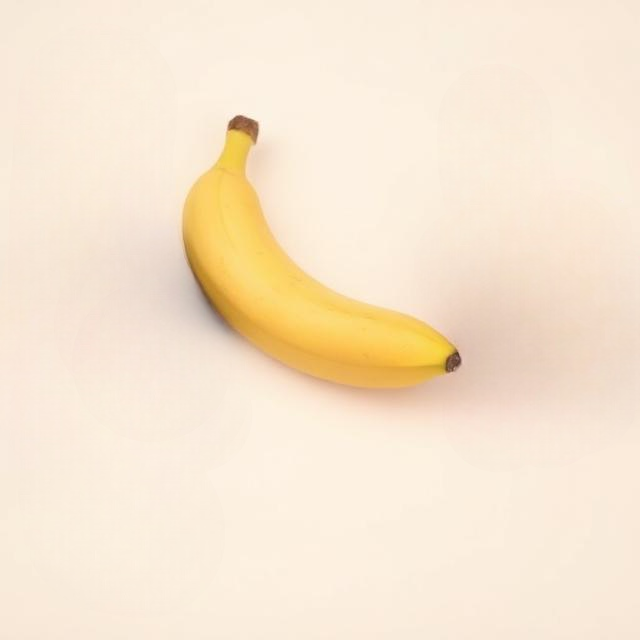
\includegraphics[width=0.33\textwidth]{figs/1a.png}
\qquad
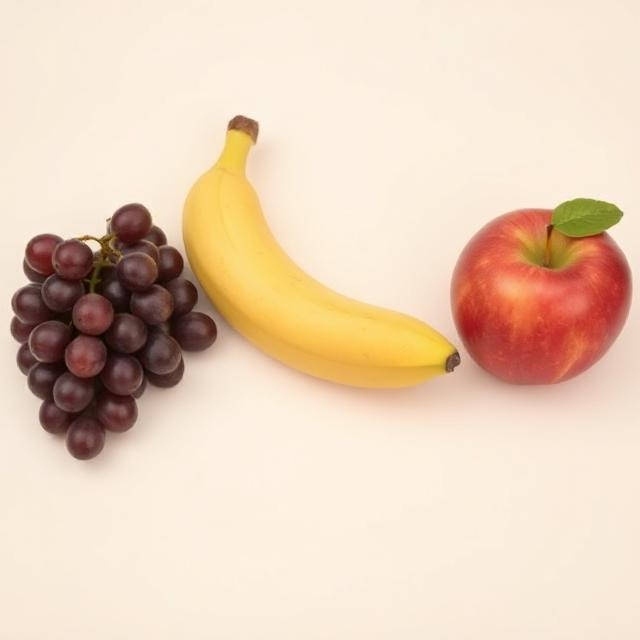
\includegraphics[width=0.33\textwidth]{figs/1b.png}
}
{\caption{Example stimuli for a sentence--picture verification task}}
\label{fig:stimuli_1}
\end{figure}


We designed a visual-world experiment with eyetracking in which participants first read a sentence and then chose between two plausible pictures: (A) a single-object image corresponding to an exhaustive interpretation, or (B) a multi-object image corresponding to a contrastive interpretation, see Figure~\ref{fig:stimuli_1} accompanying examples (\ref{ex:neutral}--\ref{ex:amongst_others}). Our main question is: How do unmodified PVF sentences (e.g., (\ref{ex:pvf})) pattern relative to the \textit{only}--exhaustive condition (ex. (\ref{ex:only})) and the \textit{amongst others}--contrastive condition (ex. (\ref{ex:amongst_others}))? We expect \textit{only} sentences to yield predominantly exhaustive choices and \textit{amongst others} sentences to favor contrastive choices; the crucial question is whether simple PVF sentences will align with one of these conditions or show a more balanced distribution. 
In addition to the choices, we record reading and reaction times and collect eye movements during the picture verification phase in order to assess whether the conditions have an impact on cognitive processing, and whether different interpretations are associated with different reaction times and/or patterns of attention. 

We hypothesize that \textit{only}-exhaustive sentences will be associated with single-object (A) images, with faster responses and more focused attention, while when presented with \textit{amongst others}-contrastive sentences, participants will prefer the multi-object (B) images and may exhibit slower responses and more distributed attention due to the presence of alternatives and the ambiguity of the underlying meaning. This would suggest that the PVF construction in itself is not exhaustive.

%%% !!!!!!!!!!!!!!!!!!!!!!!! %%%
% The question was whether the unmodified PVF sentences would pattern with the exhaustive or the contrastive condition, or if they would show a more balanced distribution of interpretations.

% When faced with \textit{unmodified} PVF sentences, if the PVF construction is inherently exhaustive, we would see people to overwhelmingly choose (A) after reading a \textit{unmodified} PVF sentence. Conversely, if the PVF construction is more naturally contrastive, we would expect a more balanced distribution of choices between the images, and potentially different patterns of eye movements reflecting the difficulty of the decision -- if it is.

%%% !!!!!!!!!!!!!!!!!!!!!!!! %%%

% distinguish
% presented
% binary choice
% best match
% context/situation
% insights
% cognitive processes
% alternatives



\subsection{Participants}


\begin{figure}[!ht]
\FIG{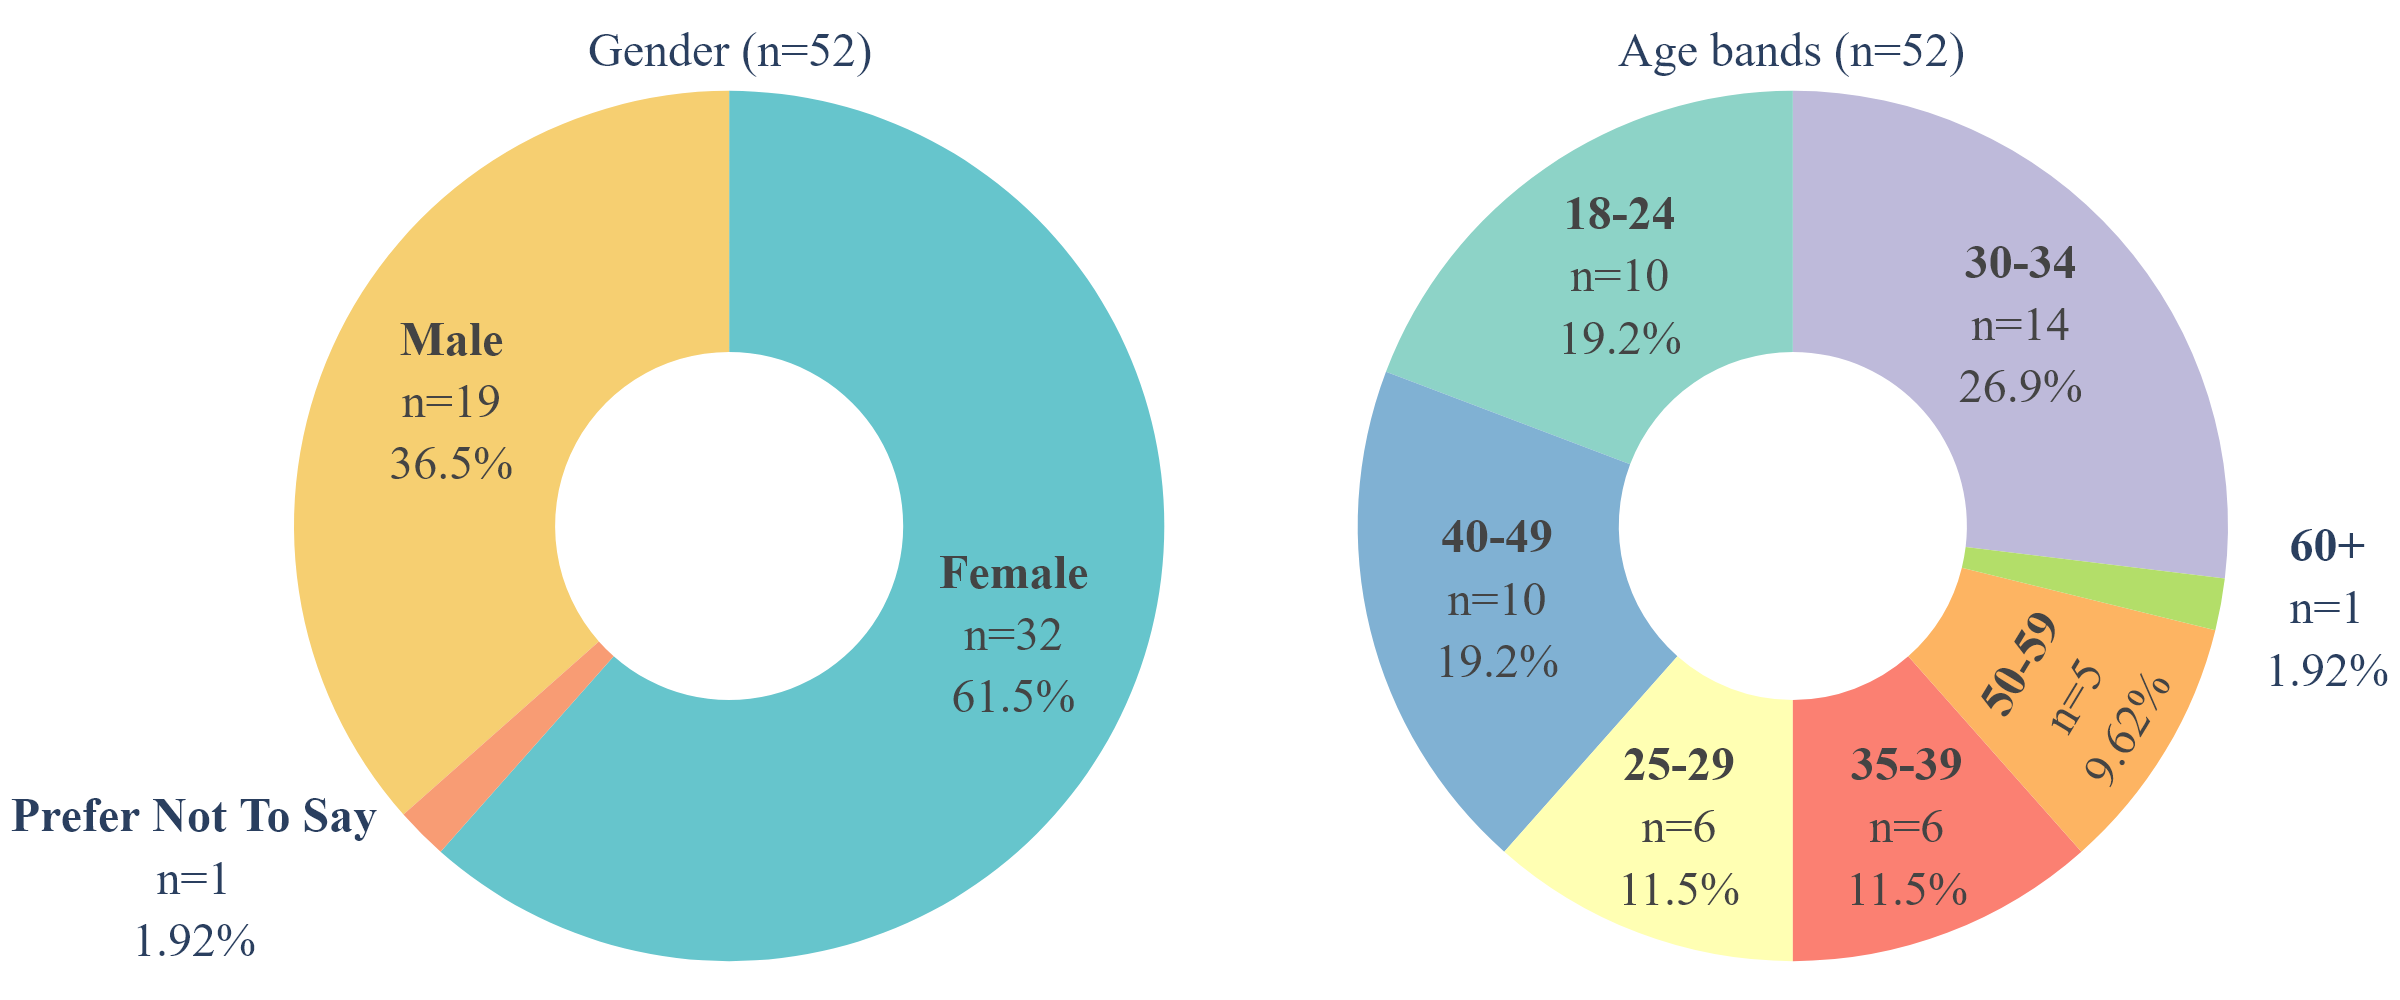
\includegraphics[width=1.0\textwidth]{figs/demographics_combined_donuts.png}}
{\caption{Demographic information of the participants in the experiment: gender (left) and age distributions (right)}
\label{demographics}}
\end{figure}


We recruited 55 native speakers of Hungarian via the Prolific platform (\url{www.prolific.com}), where participants were pre-screened for Hungarian as their first language, and received a monetary compensation for their time (around £7.50/h). After rejecting 3 participants (due to overly long submission time, failing attention checks, or missing ET data), the final sample consisted of 52 individuals (32 female; mean age = ~35). On average it took people just under 23 minutes to complete the experiment, although with a high individual variation (unusually long submission times were rejected).


\subsection{Materials}

% Materials constituted 54 sentences (18 items × 3 conditions), and 54 pairs of images with relevant single and multiple objects (Fig. 2), and 54 filler trials. Using PCIbex (Schwarz \& Zehr, 2021), we collected reading times (RT) during SPR, and eye-tracking data (total dwell time) during the SPV choice, recording the time spent looking at each target image. 

Our stimuli consisted of 54 experimental sentences (18 items × 3 conditions) with 54 additional filler sentences in a randomized order (108 in total), but making sure that the same items never followed each other. Regarding lexical variation, we used verbs both with and without verbal prefixes (50-50\%), and we included instances of both definite and indefinite conjugation (44.4-55.6\%); also, both countable and uncountable nouns were used for object focus. We added some simple contextual fillers to the beginning of each sentence, such as \textit{ami X-t illeti} `regarding X' and time or place adverbials to balance sentence length and make the targeted focus constructions appear not in the beginning of trials. When presenting the sentences on the screen, we divided them into regions, and articles were kept together with nouns, so all three conditions had the same number of regions (7), and the focused element was always in region 6 (r6). The stimuli were created by changing a set of 18 simple transitive sentences by modifying the base sentence with the addition of the focus marker \textit{csak} `only' for the exhaustive condition, and the phrase \textit{többek között} `amongst others' for the contrastive condition.

The 18 items were accompanied by 18 image pairs, these were created using DeepAI's image generator (\url{https://deepai.org/}) with prompts requesting simple 3D objects \& scenarios in front of a light pastel background, and then modified manually to get matching pairs. The full stimuli list is available online\footnote{See the Data availability statement at the end of the paper.} and in the Appendix (see the sentence list in Table \ref{tab:sentence_stimuli} and the image pairs in Fig. ~\ref{fig:visual_stimuli}). 

To avoid overly long experimental sessions, we split the experiment into three equal parts and each participant could complete one, two, or all three parts as separate events; meaning that we had three participant groups that could overlap, and each experiment consisted of 40 trials (36 experimental + 4 attention checks). This resulted in 72 valid  submissions (25 for group one, 23 for group two, and 24 for group three), thus every stimuli was interacted with at least 23 times. The three parts were split in a way that for each group each item only appeared in one condition, and each session contained four attention check questions intermixed and evenly distributed across the trials. 

The three conditions were: a) exhaustive focus with \emph{csak} `only' (e.g., (\ref{ex:stimuli_exhaustive})), b) unmodified, simple pre-verbal focus (PVF) (e.g., (\ref{ex:stimuli_pvf})), and c) contrastive focus with \emph{többek között} `amongst others' (e.g., (\ref{ex:stimuli_contrastive})). Each item was paired with two images: A) one depicting a single-object interpretation -- the exhaustive reading -- and B) one depicting a multiple-object interpretation -- the contrastive reading. See Figure~\ref{fig:stimuli_8} for an example of the image pairs accompanying the sentences in the experiment.



\begin{figure}[!ht]
\centering
\FIG{

\includegraphics[width=0.33\textwidth]{figs/8a.png}
\qquad

\includegraphics[width=0.33\textwidth]{figs/8b.png}
}
{\caption{Image pair for the sentence in examples (\ref{ex:stimuli_exhaustive}--\ref{ex:stimuli_contrastive}). The left image (A) corresponds to the exhaustive reading, while the right image (B) corresponds to the contrastive reading.}
\label{fig:stimuli_8}}
\end{figure}



\pex[everygla={},aboveglftskip=0em,interpartskip=4pt]
\a \begingl \label{ex:stimuli_exhaustive}\textbf{exhaustive focus}\\
\gla \it Ami \it az \it innivalót \it illeti, \it Eszter \it csak \it kávét \it ivott.//
\glb which{\sc [rel]} the drink-{\sc acc} regard-3{\sc sg} Eszter only coffee-{\sc acc} drink-{\sc pst}-3{\sc sg}//
\glft \quad `Regarding drinks, Eszter only drank coffee.'//
\endgl
\a \begingl \label{ex:stimuli_pvf}\textbf{unmodified pre-verbal focus}\\
\gla \it Ami \it {az innivalót} \it illeti, \it Eszter \it ma \it kávét \it ivott.//
\glb which{\sc [rel]} {the drink-{\sc acc}} regard-3{\sc sg} Eszter today coffee-{\sc acc} drink-{\sc pst}-3{\sc sg}//
\glft \quad `Regarding drinks, Eszter drank coffee today.'//
\endgl
\a \begingl \label{ex:stimuli_contrastive}\textbf{contrastive focus}\\
\gla \it Ma \it reggel \it Eszter \it többek \it között \it kávét \it ivott.//
\glb today morning Eszter others amongst coffee-{\sc acc} drink-{\sc pst}-3{\sc sg}//
\glft \quad `This morning, Eszter drank, amongst other things, coffee.'//
\endgl
\xe








\subsection{Design}



We built a sentence--picture verification (SPV) task, in which participants read a sentence and were asked to indicate the best fitting meaning-representation between two visual stimuli. First, participants saw a preview of the image pair to get familiar with the objects/context, on the left and right half of the screen (20\% of the screen's width and 40\% of the screen's height) on a canvas 50\% larger than the images to mitigate the inaccuracies of the eye tracker. After pressing the spacebar they were presented with the sentence word by word (region by region) in the middle of the screen in a self-paced reading (SPR) manner, in which participants had to use the spacebar to advance throught the sentences. We recorded reading times throughout. After reading through the sentence, the image pair re-appeared and participants had to select the image that best matched the meaning of the sentence they just read. The choice had to be made with a mouse-click anywhere on the corresponding canvas (left or right), and reaction times (RT) and eye movements were recorded during this picture verification phase. The image types were counterbalanced throughout the trials. The segments were separated by 1000 ms pauses, and after the choice, the next trial started after a brief (1000 ms) pause. The experiment was designed to be completed in around 25-30 minutes, and participants had to complete it in one setting. See Figure~\ref{fig:design} for a visual representation of the design of the experiment.

\begin{figure}[!ht]
\FIG{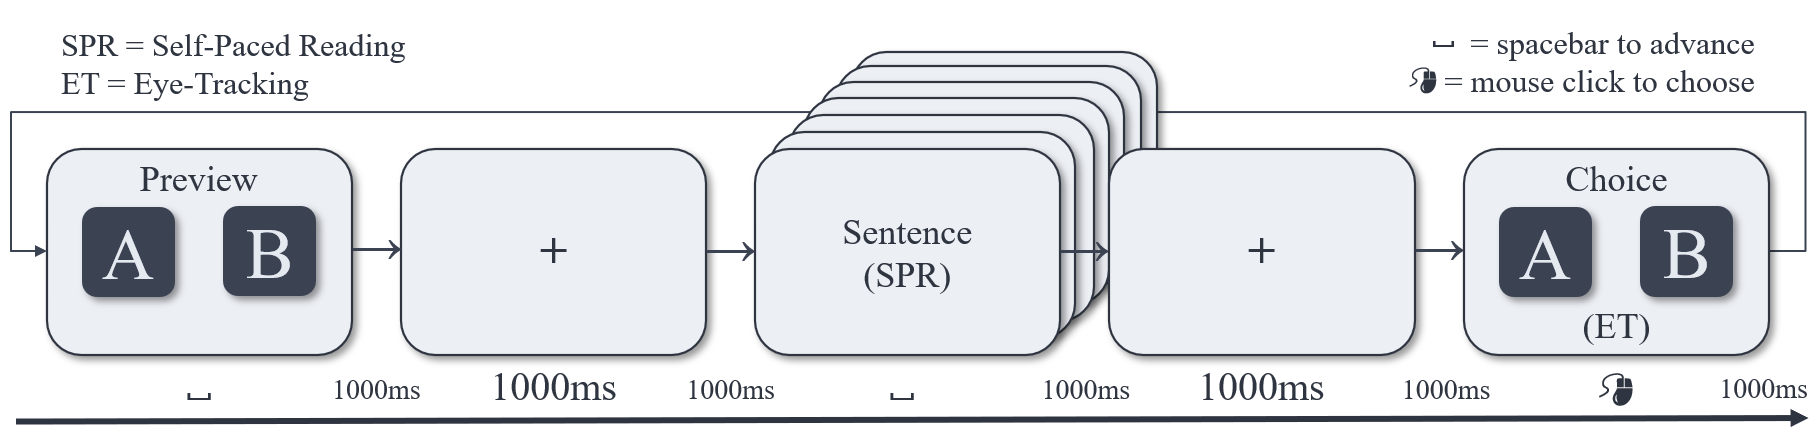
\includegraphics[width=1.0\textwidth]{figs/design.png}}
{\caption{Design}
\label{fig:design}}
\end{figure}



\subsection{Procedure}

The experiment was created, hosted on, and presented to participants on PCIbex Farm \citep{schwarz_2021_tutorial},\footnote{Code and resources are available online for inspection, see the Data availability statement at the end of the paper.} in Hungarian. Participants completed the experiment on their own devices (PC only, with a webcam and physical keyboard \& mouse) and on their own time, but with Prolific helping us control for too fast or too slow submissions resulting in rejection/timeout.

First, potential participants were instructed to be in a well-lit environment, sit at an appropriate distance from their screen and webcam, and minimize head movements; emphasizing the need for a bright location where there faces are clearly visible to the camera. They were also informed that they can only start the experiment from a Chrome browser. Before starting the experiment, participants then had to calibrate the eye tracker, which involved looking at specific points on the screen (e.g., corners, center) while the system records their eye positions to create a mapping between gaze coordinates and screen coordinates. Eye-tracking data were collected using the built-in WebGazer.js library of PCIbex, which uses the participant's webcam to track eye movements, and we used the default calibration procedure provided, a 9-point calibration grid. Participants had to reach and maintain at least 60\% accuracy in the calibration phase to proceed with the experiment, and had three attempts to achieve this accuracy, ensuring that the eye-tracking data collected during the picture verification phase would be reliable. The tracker also checked their gaze repeatedly before every trial, and if the accuracy dropped below 60\%, participants were prompted to recalibrate before proceeding to the next trial. People who could not pass the calibration for various reasons (e.g., computer setup, bad lighing/environment, glare on glasses, or any other technical issue) were not able to start the experiment. After calibration, participants were intstructed on the procedure and how to complete the task, followed by a practice session consisting of three trials, and finally they could began the live experiment of 40 trials (including 4 attention checks).

We have to mention that a relatively large amount of people (around a third of all who tried) could not pass calibration, and thus were not able to start the experiment. This is a persistent issue with webcam-based online eye tracking studies, as it can be affected by various factors such as lighting conditions, webcam quality, and even individual differences in facial features. Depending on these factors, participants' experiences were vastly different, some people breezed through trials and had a smooth experience finishing under 20 minutes, others struggled and had to recalibrate from time to time, spending over up to 40 minutes in total. We urged participants to reach out if they had issues, but sadly we couldn't assist everyone remotely. A small number of participants started but couldn't finish the experiment due to technical reasons, they were also compensated for their time, but their data was not included in the final analysis.



\subsection{Analysis}

% \subsubsection{Behavioral data?}



\subsubsection{Eye-tracking data processing}

Eye-tracking data recorded on PCIbex comes in a relatively straightforward format not of gaze coordinates but in classified samples, where each sample is already defined as a gaze at a canvas or outside the canvas, in our case: left canvas, right canvas, or neither. Samples are recorded between every ~30-70 milliseconds, depending on the users' computer \& browser setup, internet speed, and presumably the general load that the PCIbex server was under at the time.

\begin{figure}[!ht]%
\FIG{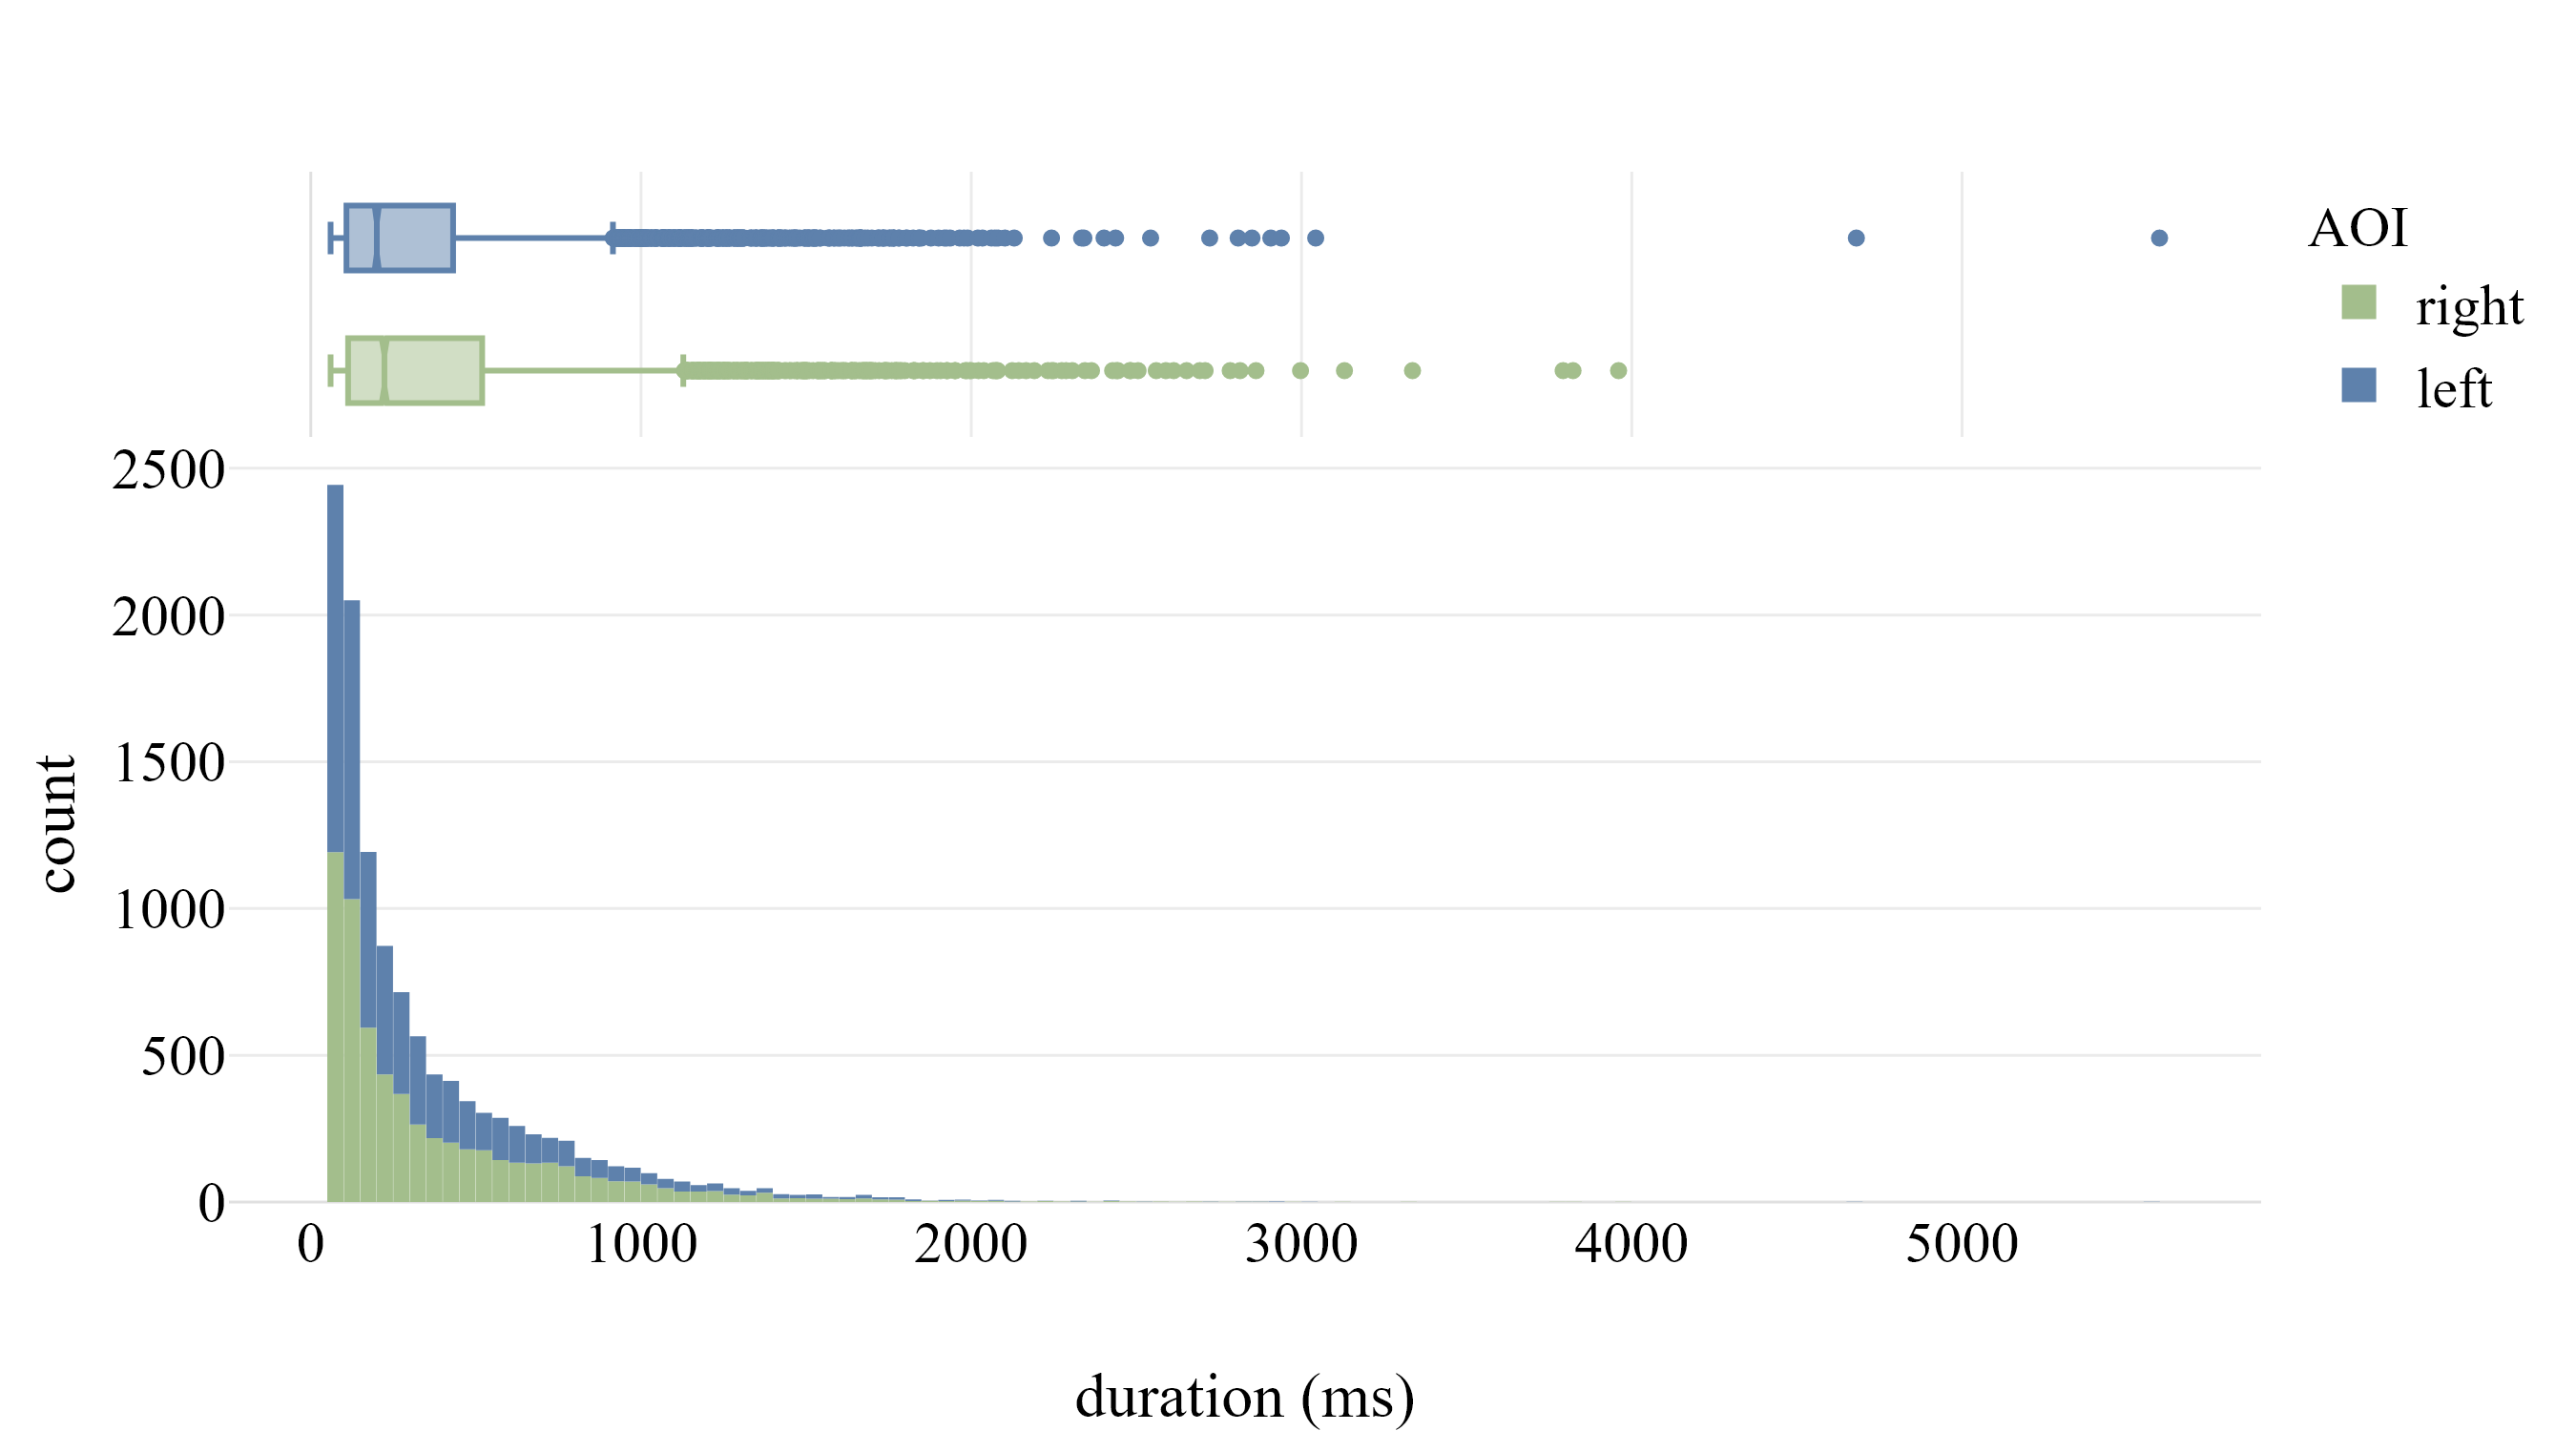
\includegraphics[width=1.0\textwidth]{figs/episodes_duration_histogram.png}}
{\caption{Distribution of episode durations after cleaning and before winsorization}
\label{fig:episodes}}
\end{figure}

The following steps were taken to clean and classify the eye-tracking data in order to obtain a certain set of metrics that could be used for analysis: First, raw eye tracking data files were loaded per participant, and \textbf{samples} were classified into AOIs at each timestamp as left (left canvas=1, right canvas=0), right (right canvas=1, left canvas=0), or neutral otherwise. Then, same-side consecutive samples were collapsed into contiguous gaze \textbf{episodes} within participant and trial. Episode duration was computed from timestamp-derived sample durations where episodes shorter than a threshold of 60 ms were removed, and neutral-gap bridging was enabled (with a max neutral bridge of 50 ms). In other words, very short gaze episodes and rapid saccades were removed cleaning noise \& jitter, as they are unlikely to reflect meaningful cognitive efforts and more likely to be artifacts of the eye-tracking system. Then, neutral episodes were dropped and excluded from further analysis. Episodes thus intend to represent a moment of sustained gaze within an AOI, ignoring brief out-of-canvas samples that result from technical inaccuracies and are not deliberate (or uncounscious) eye movements. For quality control, episode-duration distributions were inspected via summary statistics, and episodes longer than the mean +2 SD ($\mu \pm 2\sigma$) were winsorized by replacing their duration with the global mean (i.e., with rows retained). This procedure preserved the full number of episodes while limiting the influence of extreme outliers; 4.89\% of all episodes were substituted. See Figure~\ref{fig:episodes} for the distribution of episode durations. This cleaning process was devised after established eye-tracking data classification protocols, such as the Identification by Dispersion-Threshold (I-DT) algorithm, which itself is ideal for low- to mid-frequency eye trackers and static stimuli.

Finally, trial-level eye-tracking (ET) features were computed, including left/right/total dwell time, dwell proportions, dominant side, fixation counts, revisits, transitions, and first-fixation side/duration. To briefly define the most important metrics that were used in the end: \textbf{dwell} is a time value, the sum of the duration of all gaze episodes within a trial (either left, right, or total), representing the total amount of time a participant has spent looking at the AOI(s) during the choice; \textbf{fixation} on the other hand is a numeric value, representing how many times a participant looked at the AOIs during a choice. Missing trial-level metrics were mean-imputed in 5.02\% of the data points, which were mostly due to missing episode-level data (e.g., no episodes detected for a trial, or no episodes remained after cleaning).

We acknowledge that several processing decisions may limit inference. Gaze data was essentially collapsed to binary AOIs (left/right), while off-target samples were treated as neutral and excluded. Episodes shorter than 50 ms were removed, potentially excluding very brief but real events. Long-duration episodes were winsorized by replacing values above a global mean+2SD threshold with the global mean, preserving sample size but reducing variance and potentially biasing duration-based measures. Also, missing merged ET trial metrics were mean-imputed for selected variables, which further shrinks the effective sample size. We therefore interpret absolute magnitudes cautiously and focus on relative contrasts between conditions. The eye-tracking data cleaning and classification pipeline was implemented in Python, and can be inspected online with the data and results.\footnote{See the Data availability statement at the end of the paper.}



\subsubsection{Statistical analysis}

% A select few of the eye-tracking metrics were analyzed using linear mixed-effects models with FocusCondition, ChoiceType, and their interaction as fixed effects, and Participant and Item as random effects. Post-hoc comparisons were conducted using Tukey HSD tests............................

We analyzed two eye-tracking dependent measures: \textit{total dwell time} (\texttt{total\_dwell}) and \textit{total fixation count} (\texttt{total\_fixation}). For both measures, analyses were conducted in R using linear mixed-effects models (LMM) (packages \texttt{lme4}, \texttt{lmerTest}, \texttt{car}, and \texttt{emmeans}). The fixed-effect predictors were focus Condition (three levels: exhaustive, unmodified, contrastive) and image Choice (two levels: single-object, multi-object). To stabilize variance and accommodate zero values, we applied a log transform using $\log(1+x)$ to the raw dependent measure prior to modeling. For each dependent measure, we fit the following model with Participants and Items as random intercepts. The formula is: 

\begin{center}
\texttt{y' \sim~\text{Condition} * \text{Choice} + (1 \mid~\text{Participant}) + (1 \mid~\text{Item})}
\end{center}

where $y' = \log(1+y)$ is the transformed dependent variable. The models were fit using maximum likelihood estimation (i.e., \texttt{REML = FALSE}) to enable likelihood-ratio model comparisons. To follow up on significant effects in the model, we computed estimated marginal means and conducted Tukey-adjusted pairwise comparisons using \texttt{emmeans}. Specifically, we tested (i) pairwise differences between conditions within each type (Condition $\mid$ Choice), (ii) the pairwise differences between types within each condition (Choice $\mid$ Condition), and (iii) the full interplay of both (Condition $\ast$ Choice).



\section{Results}

\subsection{Behavioral results}



\begin{figure}[ht]
\FIG{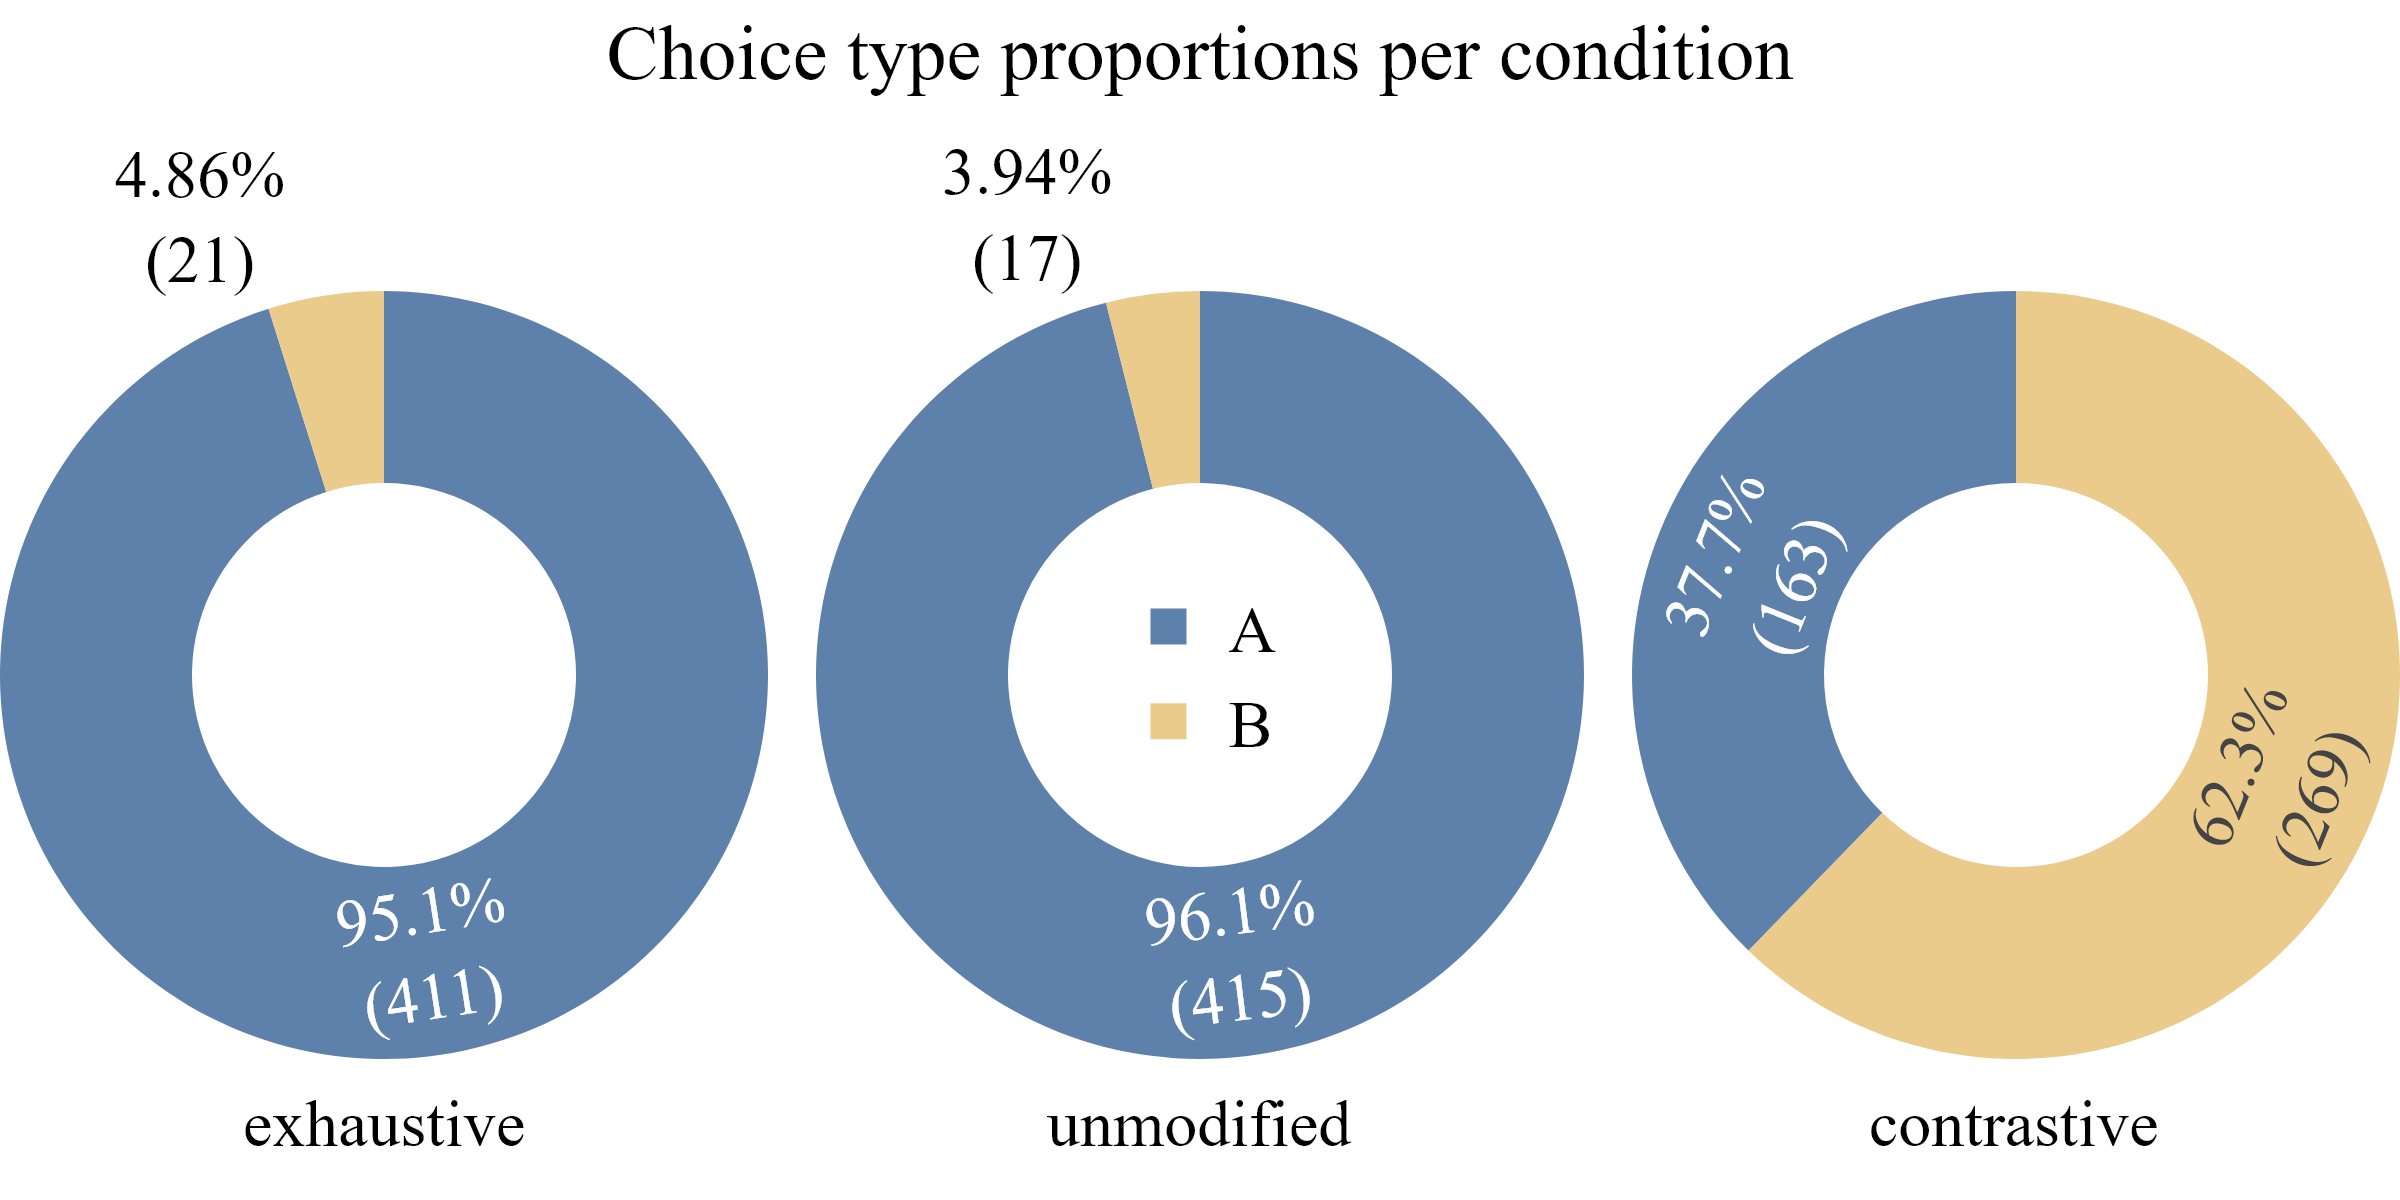
\includegraphics[width=1.0\textwidth]{figs/choice_type_per_condition.png}}
{\caption{Distribution of chosen visual stimuli (Image type A vs B) per condition}}
\label{fig:choice}
\end{figure}



\begin{table}[ht]
\centering
\caption{Type of chosen image per condition}
\label{tab:choice}
\begin{tabularx}{\textwidth}{@{}Xrr@{}}
\toprule
Condition & Image A: \% (N) & Image B: \% (N) \\
\midrule
Exhaustive   & 95.1 (411) & 4.86 (21) \\
Unmodified   & 96.1 (415) & 3.94 (17) \\
Contrastive  & 37.7 (163) & 62.3 (269) \\
\bottomrule
\end{tabularx}
\end{table}



The behavioural results showed that participants overwhelmingly interpreted the unmodified pre-verbal focus (PVF) sentences like exhaustive \textit{only}-sentences, choosing single-object type A images. However, in case of contrastive \textit{amongst others}-sentences, people preferred the multi-object type B images, exhibiting a tendency toward non-exhaustive readings, but with almost 37.7\% of the choices -- somewhat unexpectedly -- still being cast on the exhaustive interpretation type A images (see Table~\ref{tab:choice}, Figure~\ref{fig:choice}). This suggests that even with the presence of a phrase that licenses an inclusive, contrastive meaning, the exhaustivity effect is still quite salient. This pattern provides clear evidence that the PVF construction is not obligatorily interpreted as exclusively exhaustive; a non-exhaustive interpretation remains available. Our results further show that a contrastive reading can be elicited readily, and that the presence of an inclusive, contrastive licensing phrase does not fully eliminate the construction’s exhaustive bias.



\subsection{Reaction Times}

We analyzed the reading times during self-paced reading and reaction times (RT) during the picture verification phases, see the plots in Figure~\ref{fig:region_rt_by_choice_with_choice_rt_split_by_choice} for an overview. Reading times and decision reaction times were winsorized by replacing values above the mean +2 SD with the mean to mitigate the impact of extreme outliers. In the following analyses, values were log-transformed using $\log(1+x)$ to stabilize variance.

\begin{figure}[ht]
\FIG{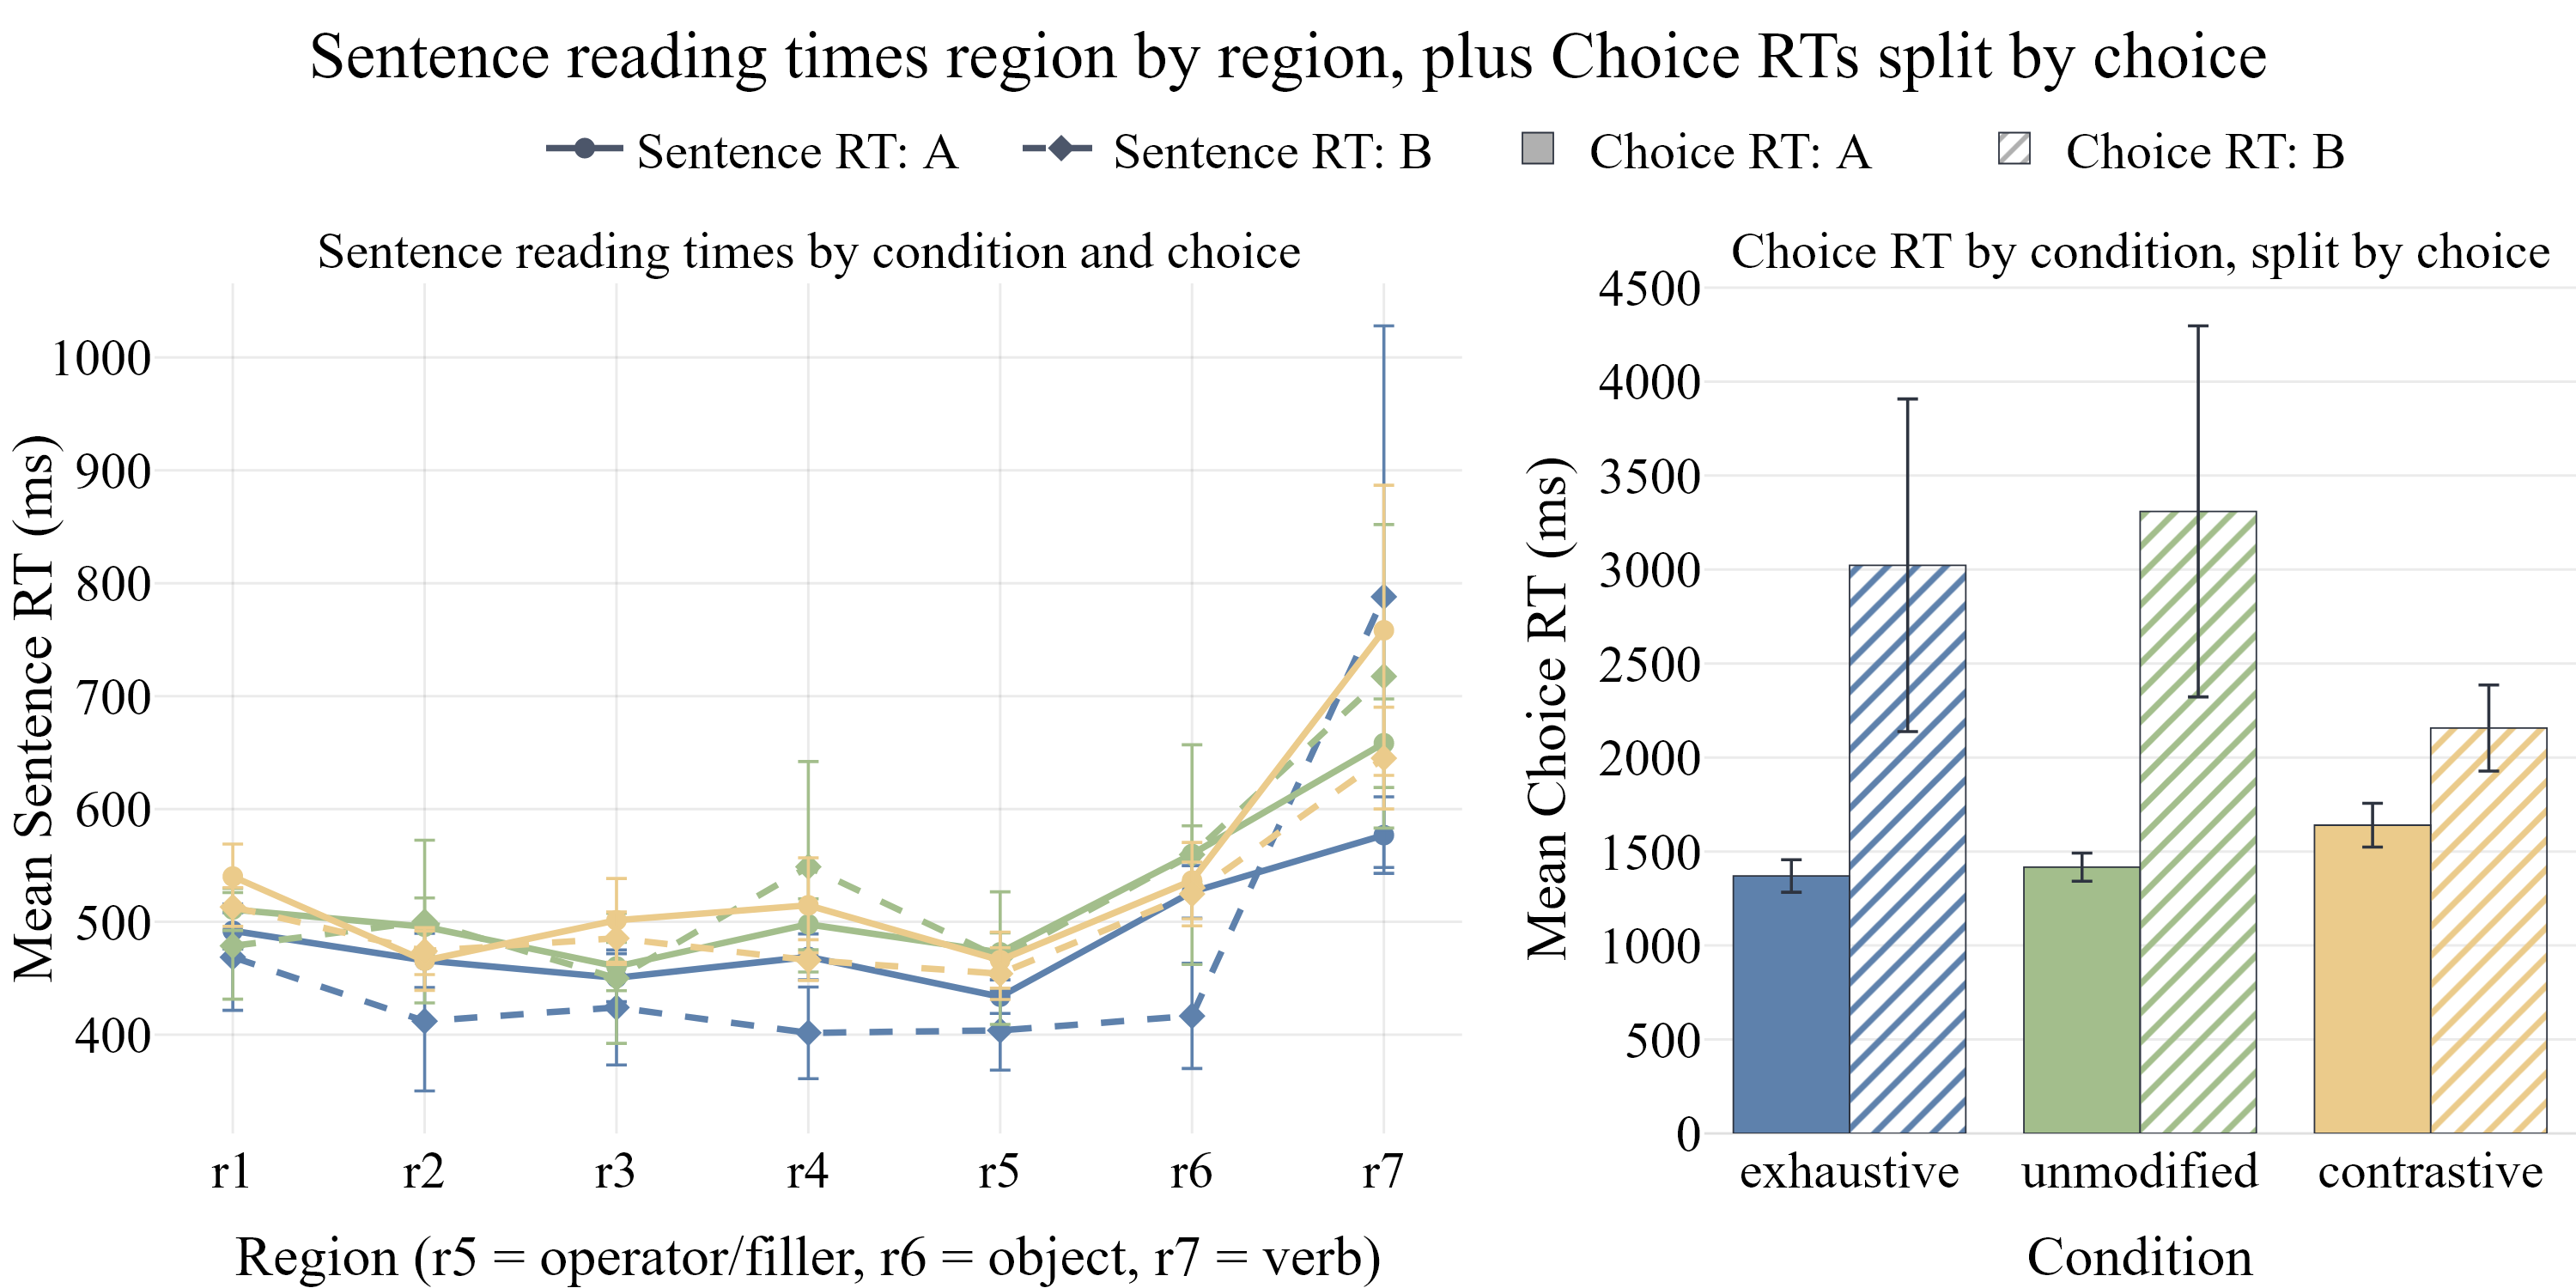
\includegraphics[width=1.0\textwidth]{figs/region_rt_by_choice_with_choice_rt_split_by_choice.png}}
{\caption{Mean reading times of sentences by regions and reaction times of choices.}}
\label{fig:region_rt_by_choice_with_choice_rt_split_by_choice}
\end{figure}



\subsubsection{Sentence Reading Times}

\begin{table}[htbp]
\centering
\caption{Type III Wald chi-square tests for whole-sentence reading times}
\label{tab:sentence-rt}
\begin{tabularx}{\textwidth}{@{}Xrrr@{}}
\toprule
Effect & $\chi^2$ & df & $p$ \\
\midrule
Condition & 18.66 & 2 & $< .001$ \\
Choice & 0.06 & 1 & .806 \\
Condition $\times$ Choice & 2.10 & 2 & .351 \\
\bottomrule
\end{tabularx}
\end{table}

For sentence reading times, the Type III Wald chi-square tests showed a significant main effect of Condition, $\chi^2(2)=18.66$, $p<.001$, but no main effect of Choice, $\chi^2(1)=0.06$, $p=.806$, and no interaction between Condition and Choice, $\chi^2(2)=2.10$, $p=.351$ (see Table~\ref{tab:sentence-rt}). This indicates that the focus condition influenced how long participants took to read the sentences, but the interpretation they ultimately settled on -- single-object or multi-object -- did not significantly affect reading times, and there was no interaction between the two factors. 

\begin{table}[htbp]
\centering
\caption{Fixed-effects tests for whole-sentence reading times, compared to \textit{exhaustive} condition and the single-object image (A) choice as reference levels}
\label{tab:sentence-rt-fixed}
\begin{tabularx}{\textwidth}{@{}Xrrrr@{}}
\toprule
Effect & Estimate & SE & df & $p$ \\
\midrule
Intercept & 8.07184 & 0.04172 & 92.77 & $< .001$ \\
Condition (unmodified) & 0.05883 & 0.01399 & 1207.28 & $< .001$ \\
Condition (contrastive) & 0.04833 & 0.01991 & 1218.66 & .015 \\
Choice B & -0.01194 & 0.04849 & 1219.95 & .806 \\
Condition (unmodified) $\times$ Choice B & -0.09711 & 0.06995 & 1214.88 & .165 \\
Condition (contrastive) $\times$ Choice B & -0.02726 & 0.05422 & 1223.36 & .615 \\
\bottomrule
\end{tabularx}
\end{table}

Relative to the exhaustive condition as the reference level, whole-sentence reading times were significantly longer in both the unmodified condition ($p<.001$) and the contrastive condition ($p=.015$). This indicates that participants read exhaustive sentences faster than both unmodified PVF sentences and contrastive \textit{amongst others}-sentences. By contrast, there was no significant effect of choice type ($p=.806$), and neither the unmodified $\times$ choice nor the contrastive $\times$ choice interaction reached significance ($p=.165$ and $p=.615$, respectively), indicating that the effect of Condition was not modulated by whether participants selected the single-object or multi-object image (see Table~\ref{tab:sentence-rt-fixed}).

\begin{table}[htbp]
\centering
\caption{Tukey-adjusted pairwise comparisons for whole-\textbf{sentence} reading times within choice type (A--A and B--B pairs)}
\label{tab:sentence-rt-pairwise-within-choice}
\begin{tabularx}{\textwidth}{@{}Xrrrrr@{}}
\toprule
Contrast & Estimate & SE & df & $t$ & $p$ \\
\midrule
Exhaustive A -- Unmodified A   & -0.05883 & 0.0140 & 1212 & -4.196 & .0004 \\
Exhaustive A -- Contrastive A  & -0.04833 & 0.0200 & 1224 & -2.422 & .1494 \\
Unmodified A -- Contrastive A  &  0.01050 & 0.0199 & 1223 &  0.529 & .9950 \\
Exhaustive B -- Unmodified B   &  0.03828 & 0.0685 & 1220 &  0.559 & .9935 \\
Exhaustive B -- Contrastive B  & -0.02106 & 0.0492 & 1225 & -0.428 & .9982 \\
Unmodified B -- Contrastive B  & -0.05935 & 0.0534 & 1221 & -1.112 & .8764 \\
\bottomrule
\end{tabularx}
\end{table}

\begin{table}[htbp]
\centering
\caption{Tukey-adjusted pairwise comparisons for whole-\textbf{sentence} reading times across choice type (A--B pairs)}
\label{tab:sentence-rt-pairwise-across-choice}
\begin{tabularx}{\textwidth}{@{}Xrrrrr@{}}
\toprule
Contrast & Estimate & SE & df & $t$ & $p$ \\
\midrule
Exhaustive A -- Exhaustive B   &  0.01194 & 0.0486 & 1225 &  0.246 & .9999 \\
Unmodified A -- Unmodified B   &  0.10905 & 0.0530 & 1223 &  2.056 & .3115 \\
Contrastive A -- Contrastive B &  0.03920 & 0.0229 & 1233 &  1.712 & .5237 \\
\bottomrule
\end{tabularx}
\end{table}



Post-hoc pairwise comparisons revealed that the significant effect of Condition was driven by significantly faster reading times in the exhaustive condition compared to the unmodified condition (\textit{p}<.001 A--A) when participants chose the expected single-object image, but not when they chose the multi-object image (\textit{p}=.994 B--B), see Table \ref{tab:sentence-rt-pairwise-within-choice}. There was no significant difference in whole sentence reading times between the exhaustive and contrastive conditions regardless of the choice type (\textit{p}=.149 A--A, \textit{p}=.998 B--B), nor between the unmodified and contrastive conditions (\textit{p}=.995 A--A; \textit{p}=.876 B--B). There was also no significance accross choice types within any of the conditions (see Table \ref{tab:sentence-rt-pairwise-across-choice}).

Taken together, this pattern of results suggests that the exhaustive focus marker \textit{csak} `only' facilitated processing relative to the unmodified PVF construction, but this advantage was limited to trials in which participants made the expected single-object choice. This indicates that the processing benefit of exhaustive marking emerged primarily when participants’ interpretations aligned with the intended exhaustive reading, and did not extend to trials in which they selected the multi-object image. At the same time, the contrastive condition with \textit{többek között} `amongst others' did not differ significantly from either the exhaustive or the unmodified condition, regardless of choice type, suggesting that the contrastive modifier did not reliably affect overall reading times. Overall, any processing advantage associated with exhaustive marking appears to have been constrained rather than general. See Figure~\ref{fig:sentence_log_rt_by_condition_split_by_choice} for a visual representation of the whole-sentence reading times by condition, split by choice type.

% facilitate
% expected

\begin{figure}[htbp]
\FIG{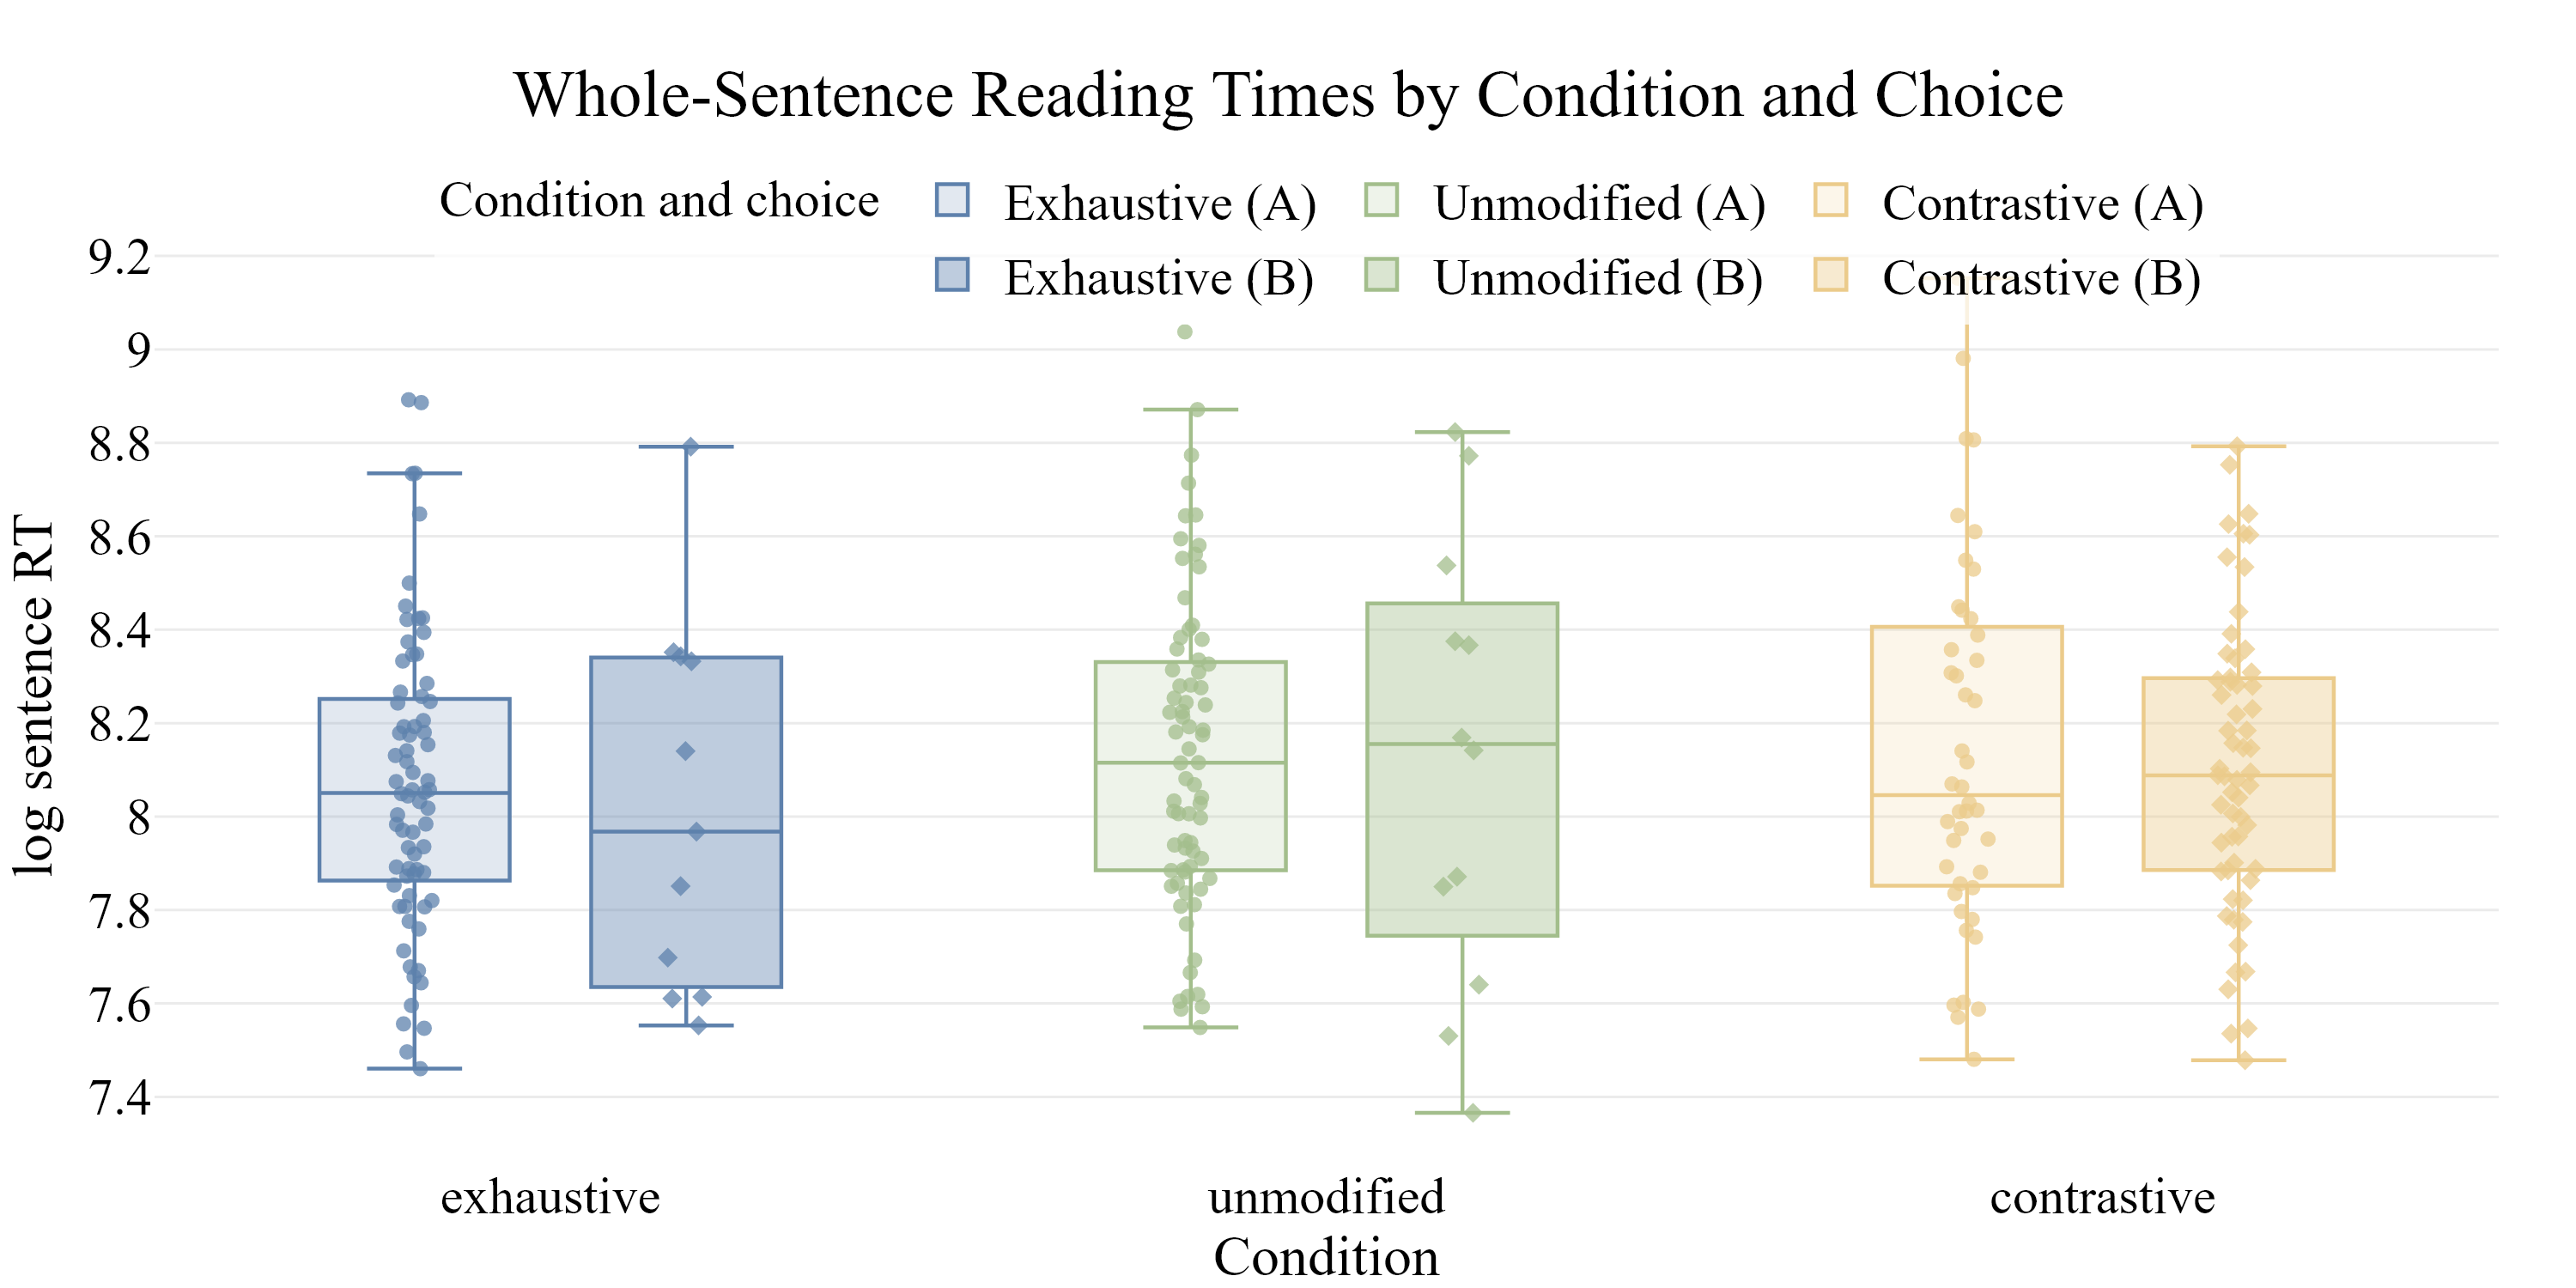
\includegraphics[width=1.0\textwidth]{figs/sentence_log_rt_by_condition_split_by_choice.png}}
{\caption{Whole-sentence reading times by condition and choice type}}
\label{fig:sentence_log_rt_by_condition_split_by_choice}
\end{figure}



\subsubsection{Regions Reading Times}

Region-level reading times were analyzed at three critical regions: r5 (containing the modifying phrases \textit{csak} `only'), a filler word, or \textit{között}, the second half of `amongst others', r6 (the focused object), and r7 (the sentence-final verb). 

%%% Region 5 %%%

\begin{table}[htbp]
\centering
\caption{Type III Wald chi-square tests for \textbf{region 5} reading times}
\label{tab:r5}
\begin{tabularx}{\textwidth}{@{}Xrrr@{}}
\toprule
Effect & $\chi^2$ & df & $p$ \\
\midrule
Condition & 18.66 & 2 & $< .001$ \\
Choice & 0.25 & 1 & .615 \\
Condition $\times$ Choice & 1.72 & 2 & .423 \\
\bottomrule
\end{tabularx}
\end{table}

\begin{table}[htbp]
\centering
\caption{Fixed effects for region 5 reading times}
\label{tab:r5-fixed}
\begin{tabularx}{\textwidth}{@{}Xrrrr@{}}
\toprule
Effect & Estimate & SE & df & $p$ \\
\midrule
Intercept & 6.02190 & 0.03691 & 95.57 & $< .001$ \\
Condition (unmodified) & 0.06953 & 0.01613 & 1207.45 & $< .001$ \\
Condition (contrastive) & 0.02961 & 0.02291 & 1226.55 & .196 \\
Chosen type B & 0.02806 & 0.05578 & 1228.78 & .615 \\
Condition (unmodified) $\times$ Chosen type B & -0.10403 & 0.08053 & 1220.48 & .197 \\
Condition (contrastive) $\times$ Chosen type B & -0.05950 & 0.06233 & 1234.24 & .340 \\
\bottomrule
\end{tabularx}
\end{table}

\noindent \textbf{Region 5.} In r5, there was a significant main effect of Condition ($p<.001$) (see Table~\ref{tab:r5}). Using the exhaustive condition as the reference level, this effect was driven by significantly faster reading times in the exhaustive condition than in the unmodified condition ($p<.001$), showing that \textit{csak} `only' was processed more quickly than the corresponding region in unmodified sentences. By contrast, the difference between the exhaustive and contrastive conditions was not significant ($p=.196$), indicating that r5 was not read significantly faster with \textit{csak} `only'than with the contrastive modifier \textit{többek között} `amongst others'. There was no significant main effect of Choice ($p=.615$), and neither interaction term reached significance (unmodified $\times$ Choice: $p=.197$; contrastive $\times$ Choice: $p=.340$), suggesting that choice type did not reliably modulate reading times in this region (see Table~\ref{tab:r5-fixed}).

% $`pairwise differences of condition, chosen_type`
%  1                             estimate     SE   df t.ratio p.value
%  exhaustive A - unmodified A   -0.06953 0.0162 1213  -4.303  0.0003[YH2.1]
%  exhaustive A - contrastive A  -0.02961 0.0230 1232  -1.289  0.7910
%  exhaustive A - exhaustive B   -0.02806 0.0559 1234  -0.502  0.9961[YH3.1]
%  exhaustive A - unmodified B    0.00644 0.0609 1230   0.106  1.0000
%  exhaustive A - contrastive B   0.00184 0.0188 1222   0.098  1.0000
%  unmodified A - contrastive A   0.03992 0.0229 1231   1.746  0.5013
%  unmodified A - exhaustive B    0.04148 0.0557 1233   0.745  0.9762
%  unmodified A - unmodified B    0.07598 0.0611 1230   1.244  0.8148
%  unmodified A - contrastive B   0.07137 0.0188 1223   3.797  0.0021
%  contrastive A - exhaustive B   0.00155 0.0574 1231   0.027  1.0000
%  contrastive A - unmodified B   0.03605 0.0631 1232   0.571  0.9929
%  contrastive A - contrastive B  0.03145 0.0263 1246   1.195  0.8392
%  exhaustive B - unmodified B    0.03450 0.0788 1225   0.438  0.9980
%  exhaustive B - contrastive B   0.02989 0.0567 1234   0.528  0.9951
%  unmodified B - contrastive B  -0.00461 0.0614 1228  -0.075  1.0000

\begin{table}[htbp]
\centering
\caption{Tukey-adjusted pairwise comparisons for \textbf{region 5} reading times within choice type (A--A and B--B pairs)}
\label{tab:r5-pairwise-within-choice}
\begin{tabularx}{\textwidth}{@{}Xrrrrr@{}}
\toprule
Contrast & Estimate & SE & df & $t$ & $p$ \\
\midrule
Exhaustive A -- Unmodified A   & -0.06953 & 0.0162 & 1213 & -4.303 & .0003 \\
Exhaustive A -- Contrastive A  & -0.02961 & 0.0230 & 1232 & -1.289 & .7910 \\
Unmodified A -- Contrastive A  &  0.03992 & 0.0229 & 1231 &  1.746 & .5013 \\
Exhaustive B -- Unmodified B   &  0.03450 & 0.0788 & 1225 &  0.438 & .9980 \\
Exhaustive B -- Contrastive B  &  0.02989 & 0.0567 & 1234 &  0.528 & .9951 \\
Unmodified B -- Contrastive B  & -0.00461 & 0.0614 & 1228 & -0.075 & 1.0000 \\
\bottomrule
\end{tabularx}
\end{table}

\begin{table}[htbp]
\centering
\caption{Tukey-adjusted pairwise comparisons for \textbf{region 5} reading times across choice type (A--B pairs)}
\label{tab:r5-pairwise-across-choice}
\begin{tabularx}{\textwidth}{@{}Xrrrrr@{}}
\toprule
Contrast & Estimate & SE & df & $t$ & $p$ \\
\midrule
Exhaustive A -- Exhaustive B   & -0.02806 & 0.0559 & 1234 & -0.502 & .9961 \\
Unmodified A -- Unmodified B   &  0.07598 & 0.0611 & 1230 &  1.244 & .8148 \\
Contrastive A -- Contrastive B &  0.03145 & 0.0263 & 1246 &  1.195 & .8392 \\
\bottomrule
\end{tabularx}
\end{table}

The Tukey-adjusted pairwise comparisons for region~5 showed that the only significant within-choice difference was between Exhaustive A and Unmodified A, with faster reading times in the exhaustive condition when participants selected image A ($p=.0003$). Across choice type, the only significant contrast was between Unmodified A and Contrastive B ($p=.0021$); all other comparisons were non-significant. Overall, this suggests that the region~5 effect was driven mainly by the contrast between exhaustive and unmodified sentences in A-choice trials. This indicates that the presence of the exhaustive focus marker \textit{csak} `only' facilitated processing of the critical region compared to the unmodified PVF construction, but this advantage was specific to trials in which participants made the expected single-object choice. The processing time of the latter half of the contrastive modifier \textit{többek között} `amongst others' did not significantly differ from either the exhaustive or unmodified conditions, suggesting that it did not reliably influence reading times in this region. 
% See Figure~\ref{fig:r5_log_rt_by_condition_split_by_choice} for a visual representation of region~5 reading times by condition and choice type.

%%% Region 6 %%%

\begin{table}[htbp]
\centering
\caption{Type III Wald chi-square tests for \textbf{region 6} reading times}
\label{tab:r6}
\begin{tabularx}{\textwidth}{@{}Xrrr@{}}
\toprule
Effect & $\chi^2$ & df & $p$ \\
\midrule
Condition & 10.52 & 2 & .005 \\
Choice & 4.52 & 1 & .034 \\
Condition $\times$ Choice & 2.37 & 2 & .306 \\
\bottomrule
\end{tabularx}
\end{table}

\begin{table}[htbp]
\centering
\caption{Fixed effects for region 6 reading times}
\label{tab:r6-fixed}
\begin{tabularx}{\textwidth}{@{}Xrrrr@{}}
\toprule
Effect & Estimate & SE & df & $p$ \\
\midrule
Intercept & 6.17005 & 0.04615 & 94.31 & $< .001$ \\
Condition (unmodified) & 0.06203 & 0.01942 & 1207.41 & .001 \\
Condition (contrastive) & 0.01699 & 0.02760 & 1225.05 & .538 \\
Chosen type B & -0.14285 & 0.06721 & 1226.73 & .034 \\
Condition (unmodified) $\times$ Chosen type B & -0.01650 & 0.09702 & 1218.93 & .865 \\
Condition (contrastive) $\times$ Chosen type B & 0.08434 & 0.07512 & 1231.93 & .262 \\
\bottomrule
\end{tabularx}
\end{table}


\noindent \textbf{Region 6.} For r6, which is the focused object, there was a significant effect of Condition ($p=.005$) and Choice ($p=.034$), but no significant interaction (see Table~\ref{tab:r6}). Using the exhaustive condition and Choice A as the reference levels, the effect of Condition was driven by a significant difference between the exhaustive and unmodified conditions ($p=.001$), whereas the exhaustive and contrastive conditions did not differ significantly ($p=.538$). The effect of Choice reflects longer reading times for Choice B than for Choice A across conditions ($p=.034$). Neither interaction term was significant (unmodified $\times$ Choice: $p=.865$; contrastive $\times$ Choice: $p=.262$), indicating that the effects of Condition and Choice were independent (see Table~\ref{tab:r6-fixed}).


Both the focus condition and the ultimate choice type independently affected reading times at the focused object, but these effects did not interact. The Condition effect reflects slower reading of the focused noun after the unmodified PVF relative to the exhaustive condition. The Choice effect reflects slower overall reading when participants went on to select the multi-object image, a pattern consistent with broader processing difficulty on trials that led to a non-default interpretation.



% $`pairwise differences of condition, chosen_type`
%  1                             estimate     SE   df t.ratio p.value
%  exhaustive A - unmodified A    -0.0620 0.0195 1212  -3.187  0.0184
%  exhaustive A - contrastive A   -0.0170 0.0277 1230  -0.614  0.9900
%  exhaustive A - exhaustive B     0.1429 0.0674 1232   2.120  0.2775
%  exhaustive A - unmodified B     0.0973 0.0734 1228   1.326  0.7709
%  exhaustive A - contrastive B    0.0415 0.0226 1221   1.834  0.4438
%  unmodified A - contrastive A    0.0450 0.0275 1229   1.635  0.5752
%  unmodified A - exhaustive B     0.2049 0.0671 1231   3.055  0.0278
%  unmodified A - unmodified B     0.1594 0.0736 1228   2.167  0.2543
%  unmodified A - contrastive B    0.1035 0.0226 1222   4.574  0.0001
%  contrastive A - exhaustive B    0.1598 0.0692 1229   2.311  0.1902
%  contrastive A - unmodified B    0.1143 0.0760 1230   1.503  0.6622
%  contrastive A - contrastive B   0.0585 0.0317 1244   1.846  0.4365
%  exhaustive B - unmodified B    -0.0455 0.0950 1224  -0.479  0.9969
%  exhaustive B - contrastive B   -0.1013 0.0683 1232  -1.485  0.6742
%  unmodified B - contrastive B   -0.0558 0.0740 1227  -0.754  0.9749



\begin{table}[htbp]
\centering
\caption{Tukey-adjusted pairwise comparisons for \textbf{region 6} reading times within choice type (A--A and B--B pairs)}
\label{tab:r6-pairwise-within-choice}
\begin{tabularx}{\textwidth}{@{}Xrrrrr@{}}
\toprule
Contrast & Estimate & SE & df & $t$ & $p$ \\
\midrule
Exhaustive A -- Unmodified A   & -0.0620 & 0.0195 & 1212 & -3.187 & .0184 \\
Exhaustive A -- Contrastive A  & -0.0170 & 0.0277 & 1230 & -0.614 & .9900 \\
Unmodified A -- Contrastive A  &  0.0450 & 0.0275 & 1229 &  1.635 & .5752 \\
Exhaustive B -- Unmodified B   & -0.0455 & 0.0950 & 1224 & -0.479 & .9969 \\
Exhaustive B -- Contrastive B  & -0.1013 & 0.0683 & 1232 & -1.485 & .6742 \\
Unmodified B -- Contrastive B  & -0.0558 & 0.0740 & 1227 & -0.754 & .9749 \\
\bottomrule
\end{tabularx}
\end{table}

\begin{table}[htbp]
\centering
\caption{Tukey-adjusted pairwise comparisons for \textbf{region 6} reading times across choice type (A--B pairs)}
\label{tab:r6-pairwise-across-choice}
\begin{tabularx}{\textwidth}{@{}Xrrrrr@{}}
\toprule
Contrast & Estimate & SE & df & $t$ & $p$ \\
\midrule
Exhaustive A -- Exhaustive B   &  0.1429 & 0.0674 & 1232 &  2.120 & .2775 \\
Unmodified A -- Unmodified B   &  0.1594 & 0.0736 & 1228 &  2.167 & .2543 \\
Contrastive A -- Contrastive B &  0.0585 & 0.0317 & 1244 &  1.846 & .4365 \\
\bottomrule
\end{tabularx}
\end{table}

Pairwise comparisons showed that the significant effect of Condition in region~6 was driven by faster reading times in the exhaustive condition than in the unmodified condition ($p=.018$), whereas the exhaustive and contrastive conditions did not differ significantly ($p=.99$). The Tukey-adjusted comparisons further showed that, within choice type, the only significant contrast was between Exhaustive A and Unmodified A ($p=.0184$). Across choice type, significant differences emerged between Unmodified A and Exhaustive B ($p=.0278$) and between Unmodified A and Contrastive B ($p=.0001$), while all other comparisons were non-significant. Taken together, these results suggest that the effect in region~6 was driven mainly by slower reading times in the unmodified condition, especially in trials involving A choices.



%%% Region 7 %%%


\begin{table}[htbp]
\centering
\caption{Type III Wald chi-square tests for region 7 reading times}
\label{tab:r7}
\begin{tabularx}{\textwidth}{@{}Xrrr@{}}
\toprule
Effect & $\chi^2$ & df & $p$ \\
\midrule
Condition & 25.48 & 2 & $< .001$ \\
Choice & 0.56 & 1 & .453 \\
Condition $\times$ Choice & 2.32 & 2 & .314 \\
\bottomrule
\end{tabularx}
\end{table}

\begin{table}[htbp]
\centering
\caption{Fixed effects for region 7 reading times}
\label{tab:r7-fixed}
\begin{tabularx}{\textwidth}{@{}Xrrrr@{}}
\toprule
Effect & Estimate & SE & df & $p$ \\
\midrule
Intercept & 6.21526 & 0.05432 & 93.39 & $< .001$ \\
Condition (unmodified) & 0.11708 & 0.02445 & 1207.52 & $< .001$ \\
Condition (contrastive) & 0.11131 & 0.03471 & 1227.70 & .001 \\
Choice B & 0.06344 & 0.08455 & 1229.31 & .453 \\
Condition (unmodified) $\times$ Choice B & -0.16501 & 0.12209 & 1220.37 & .177 \\
Condition (contrastive) $\times$ Choice B & -0.12943 & 0.09448 & 1235.24 & .171 \\
\bottomrule
\end{tabularx}
\end{table}


\noindent \textbf{Region 7.} Finishing the sentence with the unstressed verb in r7, there was a significant effect of Condition ($p<.001$), but no significant effect of Choice ($p=.453$) nor a significant interaction (see Table~\ref{tab:r7}). Using the exhaustive condition and Choice A as the reference, this effect of Condition was driven by significant differences between both the exhaustive and unmodified conditions ($p<.001$) and between the exhaustive and contrastive conditions ($p=.001$). On the other hand, Choice B did not differ significantly from Choice A ($p=.453$), and neither interaction term was significant (unmodified $\times$ Choice: $p=.177$; contrastive $\times$ Choice: $p=.171$), indicating that the effect of Condition was independent of participants' choice.


% $`pairwise differences of condition, chosen_type`
%  1                             estimate     SE   df t.ratio p.value
%  exhaustive A - unmodified A   -0.11708 0.0245 1213  -4.779  <.0001
%  exhaustive A - contrastive A  -0.11131 0.0348 1233  -3.198  0.0177[YH7.1]
%  exhaustive A - exhaustive B   -0.06344 0.0848 1234  -0.748  0.9757
%  exhaustive A - unmodified B   -0.01551 0.0924 1230  -0.168  1.0000
%  exhaustive A - contrastive B  -0.04531 0.0285 1223  -1.591  0.6047
%  unmodified A - contrastive A   0.00577 0.0346 1232   0.167  1.0000
%  unmodified A - exhaustive B    0.05364 0.0844 1233   0.636  0.9883
%  unmodified A - unmodified B    0.10157 0.0925 1230   1.098  0.8825
%  unmodified A - contrastive B   0.07177 0.0285 1223   2.519  0.1192
%  contrastive A - exhaustive B   0.04787 0.0870 1232   0.550  0.9940
%  contrastive A - unmodified B   0.09580 0.0957 1232   1.001  0.9176
%  contrastive A - contrastive B  0.06599 0.0399 1248   1.656  0.5616
%  exhaustive B - unmodified B    0.04793 0.1200 1225   0.401  0.9987
%  exhaustive B - contrastive B   0.01812 0.0859 1235   0.211  0.9999
%  unmodified B - contrastive B  -0.02980 0.0931 1229  -0.320  0.9996

% \begin{table}[htbp]
% \centering
% \caption{Tukey-adjusted pairwise comparisons for \textbf{region 7} reading times across Condition $\times$ Choice combinations}
% \label{tab:r7-pairwise}
% \begin{tabularx}{\textwidth}{@{}Xrrrrr@{}}
% \toprule
% Contrast & Estimate & SE & df & $t$ & $p$ \\
% \midrule
% Exhaustive A -- Unmodified A   & -0.11708 & 0.0245 & 1213 & -4.779 & $< .0001$ \\
% Exhaustive A -- Contrastive A  & -0.11131 & 0.0348 & 1233 & -3.198 & .0177 \\
% Exhaustive A -- Exhaustive B   & -0.06344 & 0.0848 & 1234 & -0.748 & .9757 \\
% Exhaustive A -- Unmodified B   & -0.01551 & 0.0924 & 1230 & -0.168 & 1.0000 \\
% Exhaustive A -- Contrastive B  & -0.04531 & 0.0285 & 1223 & -1.591 & .6047 \\
% Unmodified A -- Contrastive A  &  0.00577 & 0.0346 & 1232 &  0.167 & 1.0000 \\
% Unmodified A -- Exhaustive B   &  0.05364 & 0.0844 & 1233 &  0.636 & .9883 \\
% Unmodified A -- Unmodified B   &  0.10157 & 0.0925 & 1230 &  1.098 & .8825 \\
% Unmodified A -- Contrastive B  &  0.07177 & 0.0285 & 1223 &  2.519 & .1192 \\
% Contrastive A -- Exhaustive B  &  0.04787 & 0.0870 & 1232 &  0.550 & .9940 \\
% Contrastive A -- Unmodified B  &  0.09580 & 0.0957 & 1232 &  1.001 & .9176 \\
% Contrastive A -- Contrastive B &  0.06599 & 0.0399 & 1248 &  1.656 & .5616 \\
% Exhaustive B -- Unmodified B   &  0.04793 & 0.1200 & 1225 &  0.401 & .9987 \\
% Exhaustive B -- Contrastive B  &  0.01812 & 0.0859 & 1235 &  0.211 & .9999 \\
% Unmodified B -- Contrastive B  & -0.02980 & 0.0931 & 1229 & -0.320 & .9996 \\
% \bottomrule
% \end{tabularx}
% \end{table}

\begin{table}[htbp]
\centering
\caption{Tukey-adjusted pairwise comparisons for \textbf{region 7} reading times within choice type (A--A and B--B pairs)}
\label{tab:r7-pairwise-within-choice}
\begin{tabularx}{\textwidth}{@{}Xrrrrr@{}}
\toprule
Contrast & Estimate & SE & df & $t$ & $p$ \\
\midrule
Exhaustive A -- Unmodified A   & -0.11708 & 0.0245 & 1213 & -4.779 & $< .0001$ \\
Exhaustive A -- Contrastive A  & -0.11131 & 0.0348 & 1233 & -3.198 & .0177 \\
Unmodified A -- Contrastive A  &  0.00577 & 0.0346 & 1232 &  0.167 & 1.0000 \\
Exhaustive B -- Unmodified B   &  0.04793 & 0.1200 & 1225 &  0.401 & .9987 \\
Exhaustive B -- Contrastive B  &  0.01812 & 0.0859 & 1235 &  0.211 & .9999 \\
Unmodified B -- Contrastive B  & -0.02980 & 0.0931 & 1229 & -0.320 & .9996 \\
\bottomrule
\end{tabularx}
\end{table}

\begin{table}[htbp]
\centering
\caption{Tukey-adjusted pairwise comparisons for \textbf{region 7} reading times across choice type (A--B pairs)}
\label{tab:r7-pairwise-across-choice}
\begin{tabularx}{\textwidth}{@{}Xrrrrr@{}}
\toprule
Contrast & Estimate & SE & df & $t$ & $p$ \\
\midrule
Exhaustive A -- Exhaustive B   & -0.06344 & 0.0848 & 1234 & -0.748 & .9757 \\
Exhaustive A -- Unmodified B   & -0.01551 & 0.0924 & 1230 & -0.168 & 1.0000 \\
Exhaustive A -- Contrastive B  & -0.04531 & 0.0285 & 1223 & -1.591 & .6047 \\
Unmodified A -- Exhaustive B   &  0.05364 & 0.0844 & 1233 &  0.636 & .9883 \\
Unmodified A -- Unmodified B   &  0.10157 & 0.0925 & 1230 &  1.098 & .8825 \\
Unmodified A -- Contrastive B  &  0.07177 & 0.0285 & 1223 &  2.519 & .1192 \\
Contrastive A -- Exhaustive B  &  0.04787 & 0.0870 & 1232 &  0.550 & .9940 \\
Contrastive A -- Unmodified B  &  0.09580 & 0.0957 & 1232 &  1.001 & .9176 \\
Contrastive A -- Contrastive B &  0.06599 & 0.0399 & 1248 &  1.656 & .5616 \\
\bottomrule
\end{tabularx}
\end{table}



Post-hoc pairwise comparisons showed that the significant effect of Condition in region~7 was driven by faster reading times in the exhaustive condition than in both the unmodified condition ($p<.001$) and the contrastive condition ($p=.0177$), while the unmodified and contrastive conditions did not differ significantly. The Tukey-adjusted comparisons further indicated that these differences were restricted to A-choice trials: within choice type, only Exhaustive A vs.\ Unmodified A and Exhaustive A vs.\ Contrastive A were significant, whereas all B--B and A--B comparisons were non-significant. Taken together, these results suggest that the effect in the final region was driven primarily by faster reading times in the exhaustive condition when participants selected image A, consistent with the idea that the final region reflects the cumulative effect of the preceding sentence on comprehension.



\subsubsection{Decision Reaction Times}

\begin{table}[htbp]
\centering
\caption{Type III Wald chi-square tests for choice reaction times}
\label{tab:choice-rt}
\begin{tabularx}{\textwidth}{@{}Xrrr@{}}
\toprule
Effect & $\chi^2$ & df & $p$ \\
\midrule
Condition & 5.24 & 2 & .073 \\
Choice & 7.66 & 1 & .006 \\
Condition $\times$ Choice & 4.30 & 2 & .117 \\
\bottomrule
\end{tabularx}
\end{table}

\begin{table}[htbp]
\centering
\caption{Fixed effects for choice reading times}
\label{tab:choice-rt-fixed}
\begin{tabularx}{\textwidth}{@{}Xrrrr@{}}
\toprule
Effect & Estimate & SE & df & $p$ \\
\midrule
Intercept & 7.04055 & 0.06940 & 48.87 & $< .001$ \\
Condition (unmodified) & 0.05097 & 0.03034 & 1207.63 & .093 \\
Condition (contrastive) & 0.08833 & 0.04301 & 1235.44 & .040 \\
Choice B & 0.29001 & 0.10478 & 1235.50 & .006 \\
Condition (unmodified) $\times$ Choice B & -0.07690 & 0.15146 & 1223.09 & .612 \\
Condition (contrastive) $\times$ Choice B & -0.22380 & 0.11701 & 1243.58 & .056 \\
\bottomrule
\end{tabularx}
\end{table}

For decision reaction times, the Type III Wald chi-square tests revealed a significant main effect of Choice ($p=.006$), a marginal main effect of Condition ($p=.073$), and no significant Condition $\times$ Choice interaction ($p=.117$) (see Table~\ref{tab:choice-rt}). Unlike sentence reading times, which varied primarily by condition, decision times were primarily driven by the type of image selected, with multi-object choices taking longer than single-object choices.

% This suggests that the task itself has influence on the decision time, unlike while previously, as expected, the choice did not show significant influence on reading times.

Using the exhaustive condition and Choice~A as the reference levels, the model showed that decision times were significantly longer in the contrastive condition than in the exhaustive condition ($p=.040$), whereas the unmodified condition did not differ significantly from the exhaustive condition ($p=.093$). Choice~B responses were significantly slower than Choice~A responses ($p=.006$). The marginal contrastive $\times$ Choice interaction ($p=.056$), together with the non-significant unmodified $\times$ Choice interaction ($p=.612$), suggests that the A--B difference may be somewhat reduced in the contrastive condition.



% $`pairwise differences of condition, chosen_type`
%  1                             estimate     SE   df t.ratio p.value
%  exhaustive A - unmodified A    -0.0489 0.0335 1213  -1.458  0.6910[YH9.1]
%  exhaustive A - contrastive A   -0.1325 0.0476 1241  -2.786  0.0604[YH10.1]
%  exhaustive A - exhaustive B    -0.3774 0.1160 1242  -3.256  0.0147[YH11.1]
%  exhaustive A - unmodified B    -0.2769 0.1260 1236  -2.192  0.2422
%  exhaustive A - contrastive B   -0.1822 0.0390 1227  -4.677  <.0001
%  unmodified A - contrastive A   -0.0836 0.0474 1240  -1.765  0.4889
%  unmodified A - exhaustive B    -0.3284 0.1150 1240  -2.847  0.0510
%  unmodified A - unmodified B    -0.2280 0.1270 1237  -1.801  0.4651
%  unmodified A - contrastive B   -0.1333 0.0390 1228  -3.421  0.0084
%  contrastive A - exhaustive B   -0.2449 0.1190 1238  -2.058  0.3103
%  contrastive A - unmodified B   -0.1444 0.1310 1238  -1.104  0.8800
%  contrastive A - contrastive B  -0.0497 0.0544 1262  -0.915  0.9428
%  exhaustive B - unmodified B     0.1005 0.1640 1228   0.614  0.9900
%  exhaustive B - contrastive B    0.1951 0.1170 1242   1.662  0.5570
%  unmodified B - contrastive B    0.0947 0.1270 1235   0.744  0.9764



\begin{table}[htbp]
\centering
\caption{Tukey-adjusted pairwise comparisons for \textbf{choice reaction times} within choice type (A--A and B--B pairs)}
\label{tab:choice-rt-pairwise-within-choice}
\begin{tabularx}{\textwidth}{@{}Xrrrrr@{}}
\toprule
Contrast & Estimate & SE & df & $t$ & $p$ \\
\midrule
Exhaustive A -- Unmodified A   & -0.0510 & 0.0304 & 1213 & -1.676 & .5478 \\
Exhaustive A -- Contrastive A  & -0.0883 & 0.0431 & 1241 & -2.049 & .3154 \\
Unmodified A -- Contrastive A  & -0.0374 & 0.0429 & 1239 & -0.870 & .9535 \\
Exhaustive B -- Unmodified B   &  0.0259 & 0.1480 & 1228 &  0.175 & 1.0000 \\
Exhaustive B -- Contrastive B  &  0.1355 & 0.1060 & 1241 &  1.273 & .7997 \\
Unmodified B -- Contrastive B  &  0.1095 & 0.1150 & 1234 &  0.949 & .9335 \\
\bottomrule
\end{tabularx}
\end{table}

\begin{table}[htbp]
\centering
\caption{Tukey-adjusted pairwise comparisons for \textbf{choice reaction times} across choice type (A--B pairs)}
\label{tab:choice-rt-pairwise-across-choice}
\begin{tabularx}{\textwidth}{@{}Xrrrrr@{}}
\toprule
Contrast & Estimate & SE & df & $t$ & $p$ \\
\midrule
Exhaustive A -- Exhaustive B   & -0.2900 & 0.1050 & 1241 & -2.761 & .0646 \\
Unmodified A -- Unmodified B   & -0.2131 & 0.1150 & 1236 & -1.858 & .4290 \\
Contrastive A -- Contrastive B & -0.0662 & 0.0493 & 1261 & -1.343 & .7607 \\
\bottomrule
\end{tabularx}
\end{table}

The Tukey-adjusted pairwise comparisons refine this pattern. Within Choice~A, no between-condition comparison reached significance after adjustment. Within Choice~B, no pairwise differences between conditions were significant (all $p$s $\ge .800$). 
Within conditions, none of the A--B contrasts reached significance after Tukey correction: exhaustive ($p=.065$), unmodified ($p=.429$), and contrastive ($p=.761$). Taken together, decision times for A and B choices did not differ significantly within any condition after Tukey correction (exhaustive: $p=.065$, a marginal trend; unmodified: $p=.429$; contrastive: $p=.761$). This pattern suggests that, once participants had settled on a particular interpretation, the speed of that decision was not strongly differentiated by whether the chosen image was the expected one or not -- pointing to both readings remaining accessible across all three conditions.



\begin{figure}[htbp]
\FIG{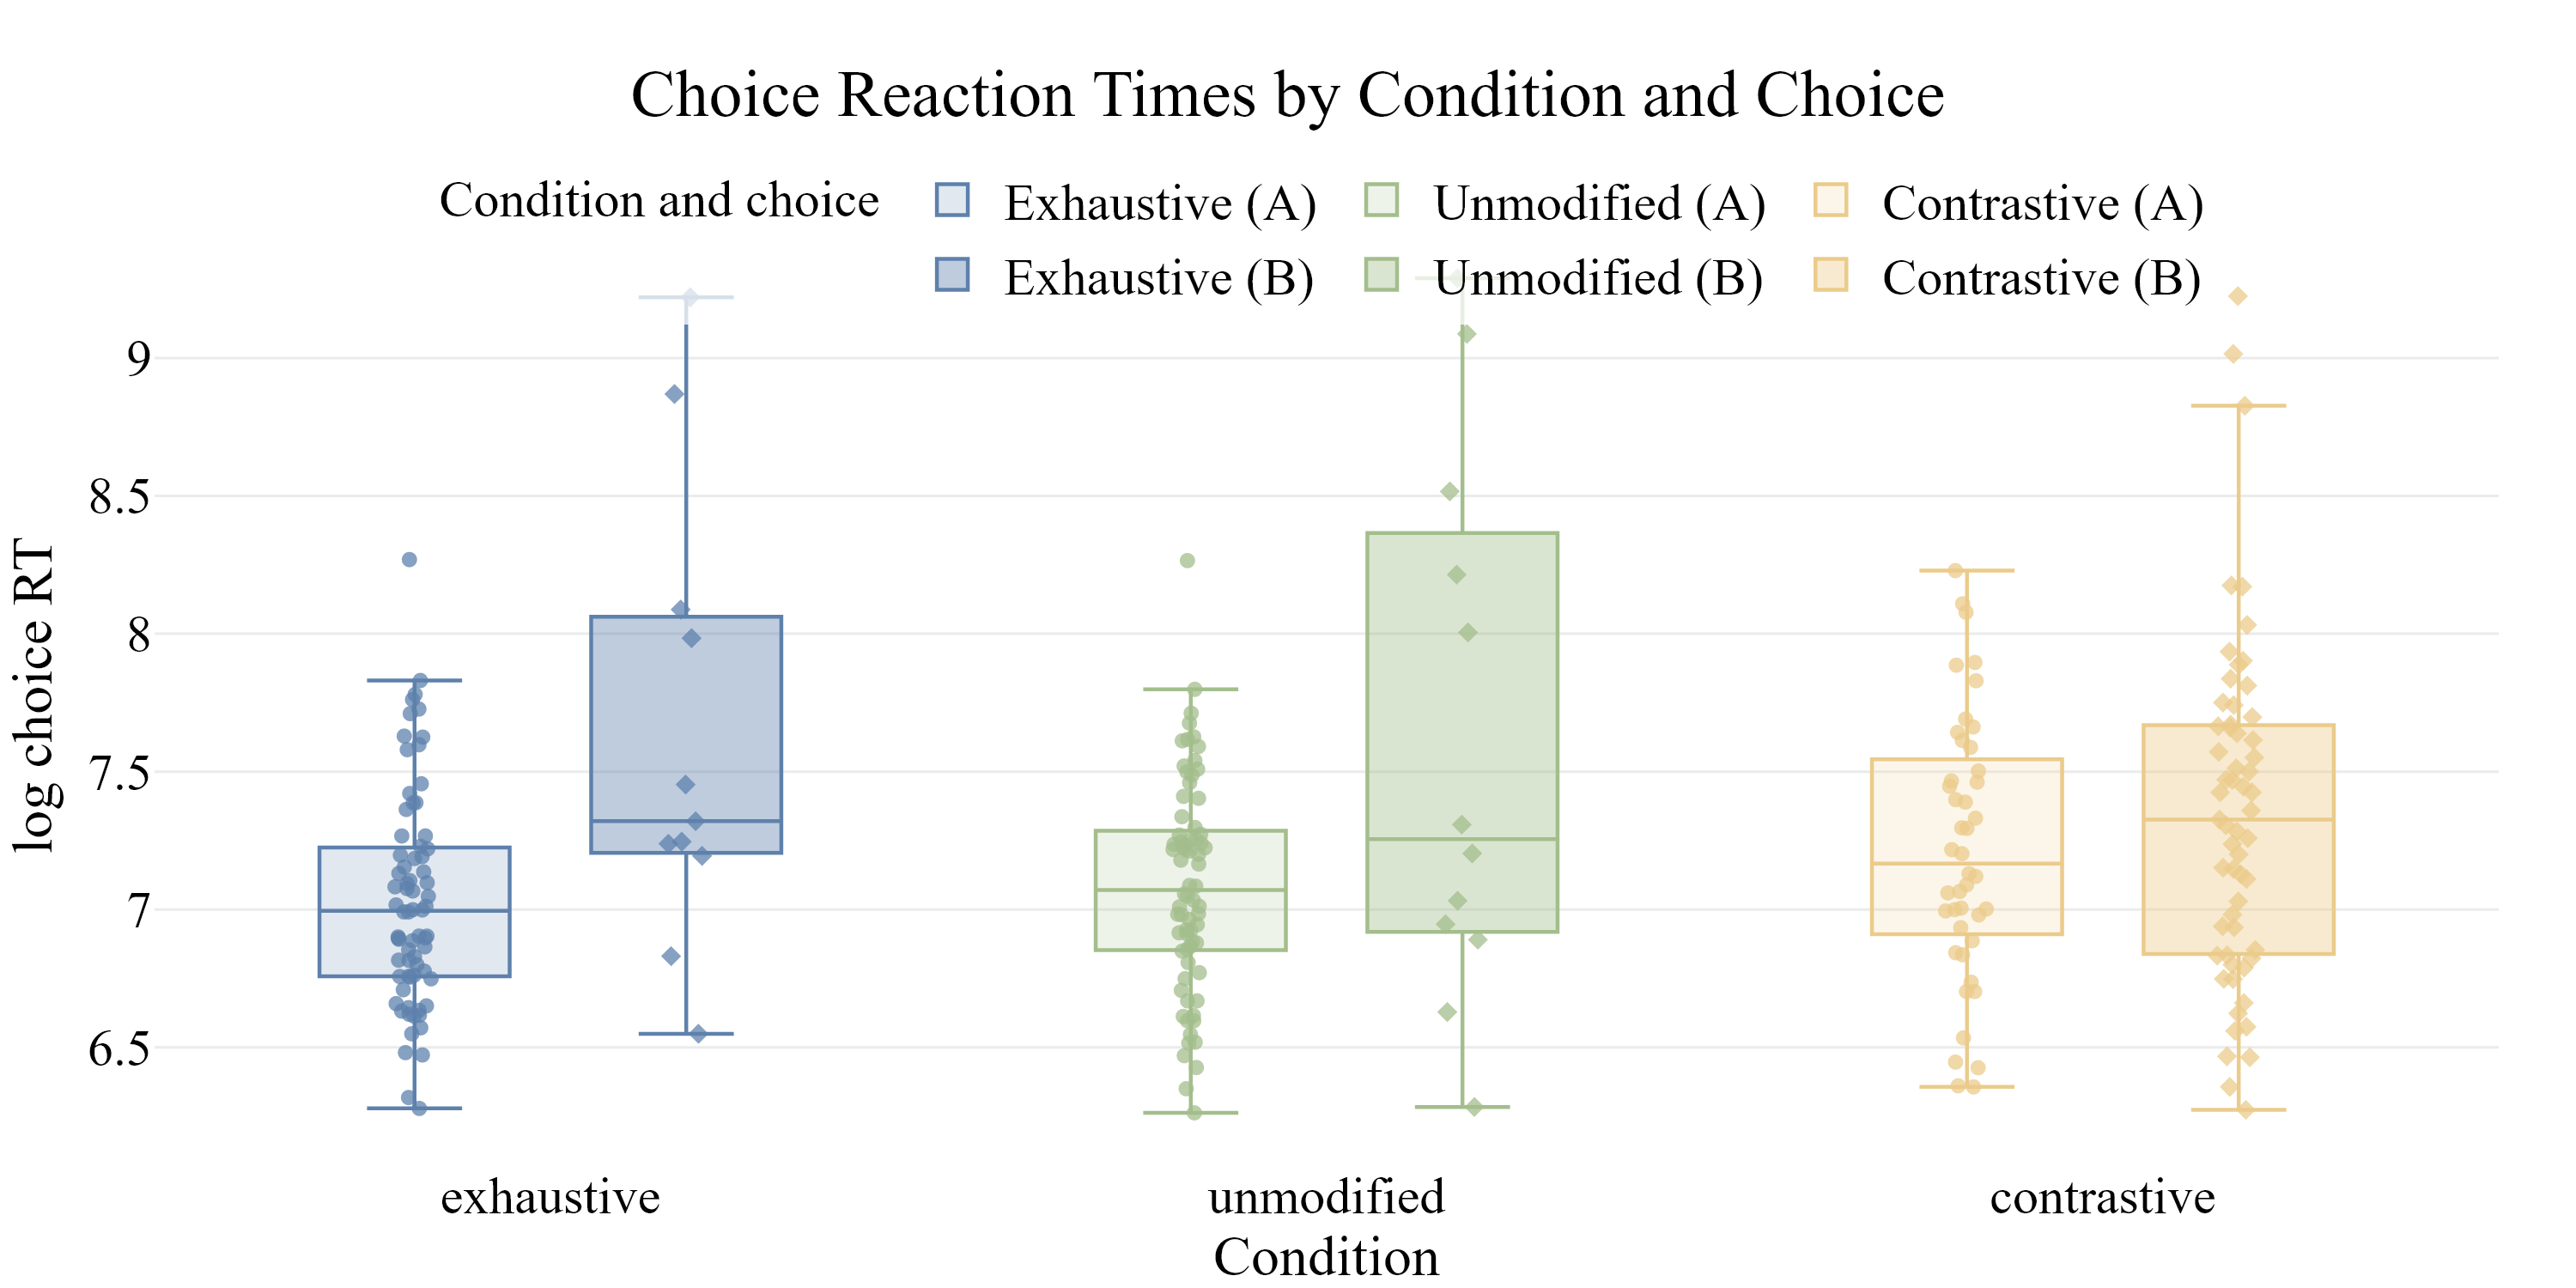
\includegraphics[width=1.0\textwidth]{figs/log_choice_rt_by_condition_split_by_choice.png}}
{\caption{Choice reaction times by condition, split by choice}}
\label{fig:log_choice_rt_by_condition_split_by_choice}
\end{figure}


% FROM ABSTRACT
% Conditions significantly influence sentences’ overall RTs: exhaustive sentences were read faster than unmodified (p<.0001) and contrastive sentences (p<.05). Pairwise comparisons showed that only-sentences were read especially fast when compared to unmodified sentences when people chose A (p=.0004). During word-by-word processing, in region corresponding to ‘only’, participants read this region significantly quicker than in unmodified condition (p=.0003); this same pattern was found in the object region (p=.0184), and the sentence-final region (p<.0001). Additionally, while other pairwise comparisons were insignificant, the sentence-final region was read faster when readers selected A in the exhaustive condition, i.e., explicit exhaustive readings were facilitated. The task also influenced the reaction times of choice. Effects were found on the Choice (p=.001), the Condition (p=.018) and in their interaction (p=.029): Decision-making was quicker in the exhaustive condition than in the contrastive condition (p=.005) regardless of selecting A or B (ps >.06), but it was not significantly different from the unmodified condition (p=.144). In short, RT results show that explicit exhaustive focus denotation facilitated the reading

% comprehension, unlike the unmodified condition; however, to make a decision, the RTs needed between exhaustive and unmodified was not significantly different.



\subsection{Eye-tracking results}



\begin{table*}[t] % use table (not table*) if your document is single-column
\centering
\caption{Type-III Wald $\chi^2$ tests from mixed models}
\label{tab:omnibus}
\begin{tabularx}{\textwidth}{@{} l X r r l @{}}
\toprule
Metric & Effect & $\chi^2$ & df & $p$ \\
\midrule
total\_dwell    & condition               & 12.531 & 2 & .0019 **~ \\
                & choice            & 11.845 & 1 & .0006 *** \\
                & condition $\times$ choice & 12.292 & 2 & .0021 **~ \\
\midrule
total\_fixation & condition               & 12.326 & 2 & .0021 ** \\
                & choice            & 3.346  & 1 & .0674 .~ \\
                & condition $\times$ choice & 6.764  & 2 & .0340 *~ \\
\bottomrule
\end{tabularx}
\end{table*}



To further examine how the focus structures were associated with exhaustive and contrastive readings, and how the conditions and choices influenced cognitive processing, we fitted linear mixed-effects models to two eye-tracking metrics: \textit{total dwell time}, and \textit{total fixation count} with fixed effects of Condition (exclusive--\textit{only}, unmodified, and contrastive--\textit{among others}), Choice (single- vs multi-object type images), and their interaction, with random intercepts for Participant and Item. Dependent variables were log-transformed using \texttt{log1p} here as well. Type-III Wald $\chi^2$ tests and Tukey-adjusted pairwise comparisons from \texttt{emmeans} were used for inference.

\subsubsection{Dwell times}

% Figure of log_total_dwell_by_condition_and_choice.png
\begin{figure}
\FIG{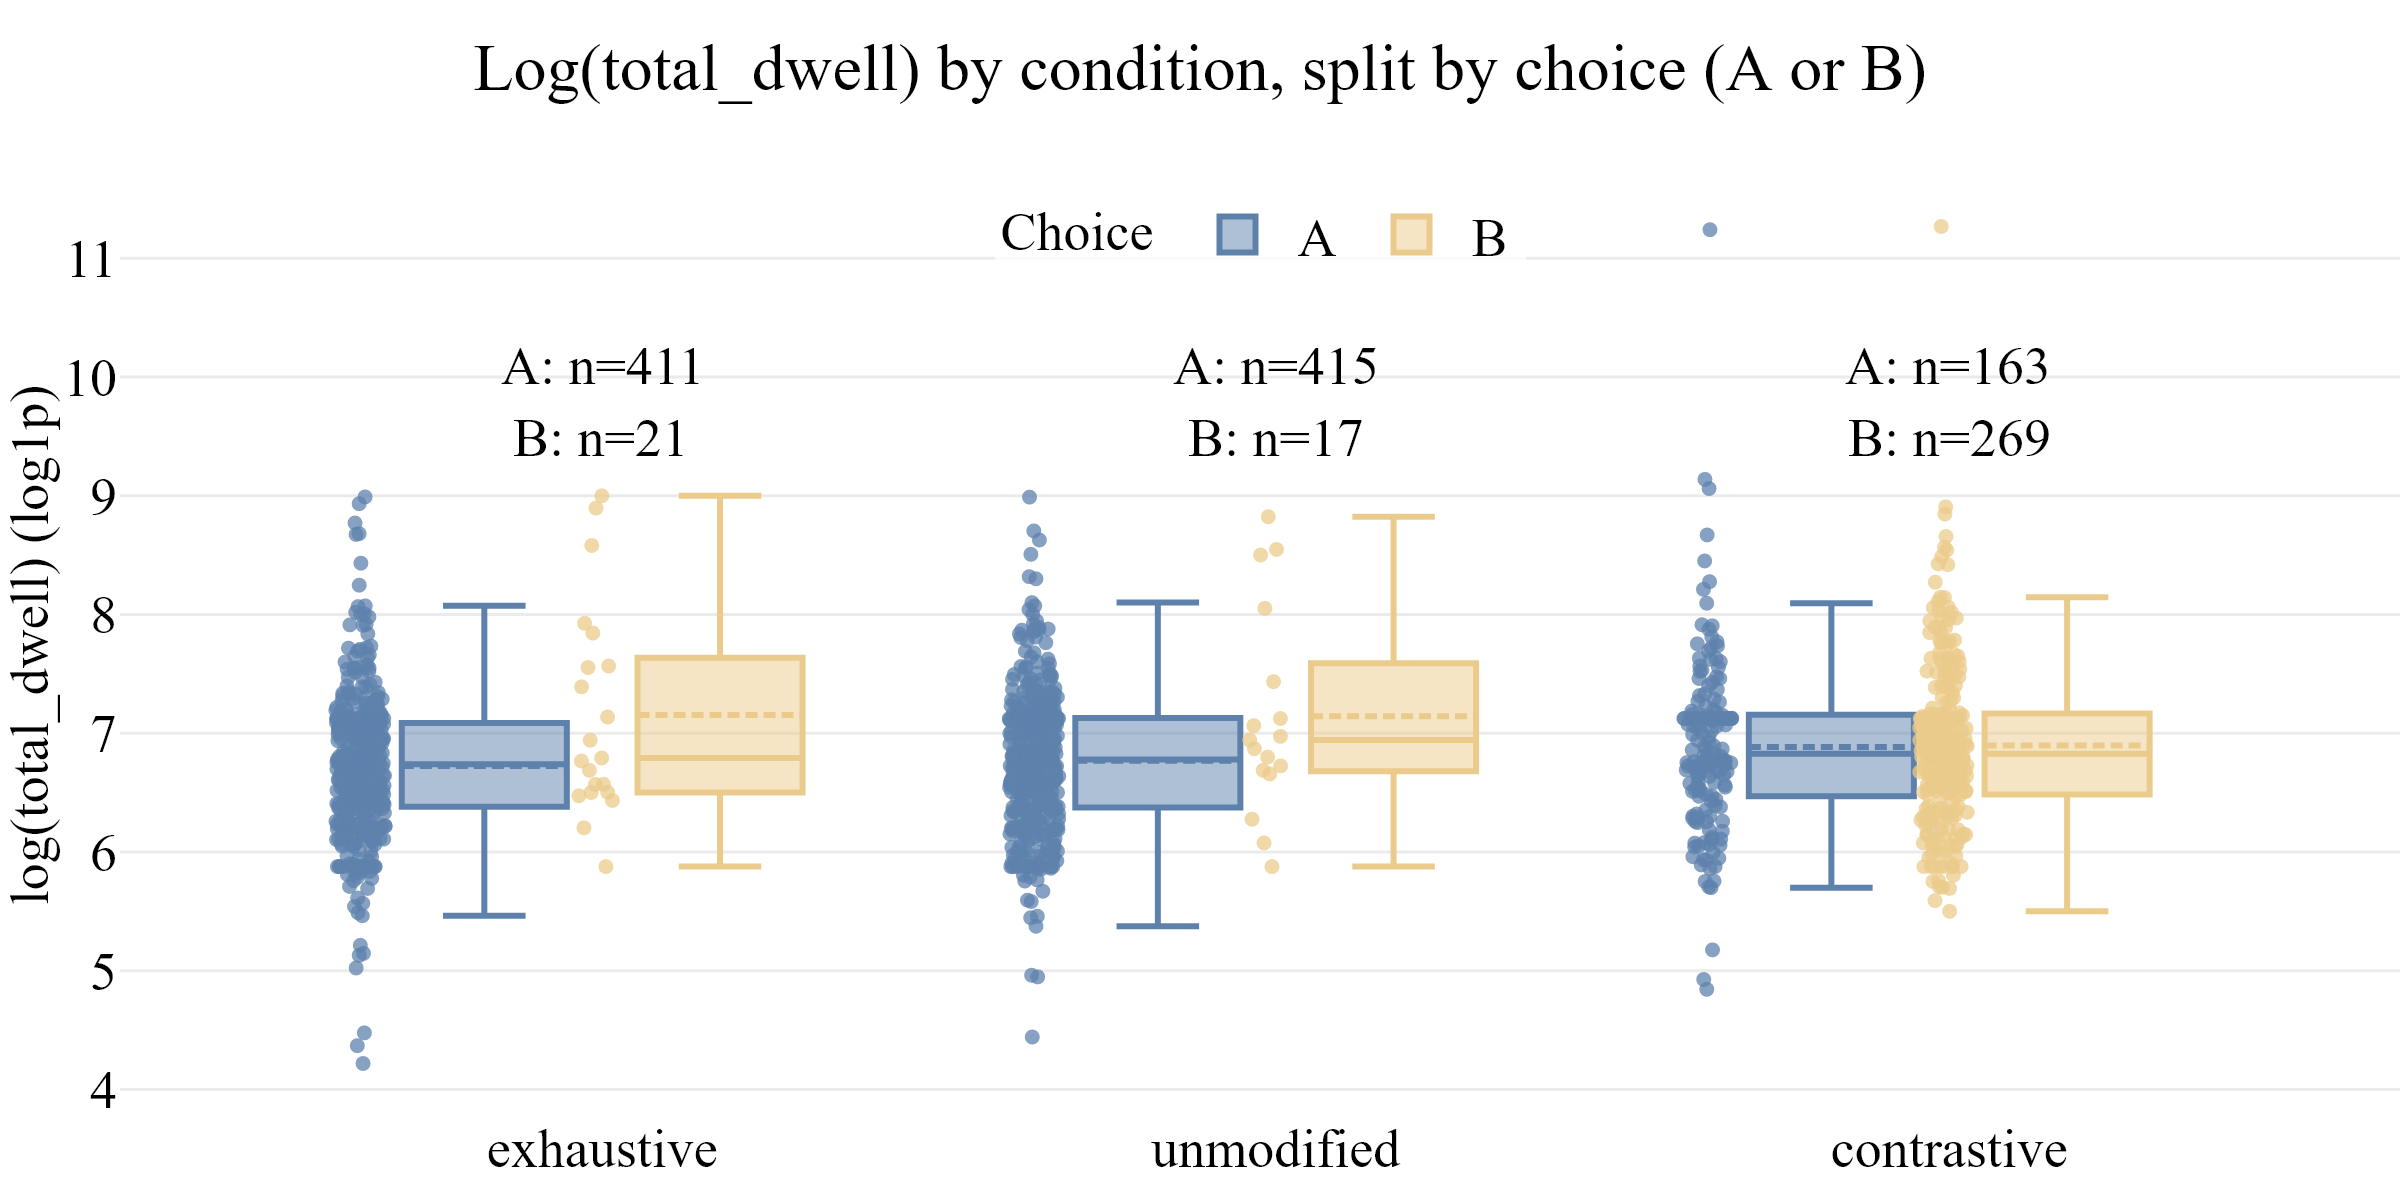
\includegraphics[width=1.0\textwidth]{figs/log_total_dwell_by_condition_and_choice.png}}
{\caption{Total dwell time (log-transformed) by condition and choice type}}
\label{fig:dwell}
\end{figure}



\begin{table}[htbp]
\centering
\caption{Type III Wald chi-square tests for total dwell time}
\label{tab:total-dwell}
\begin{tabularx}{\textwidth}{@{}Xrrr@{}}
\toprule
Effect & $\chi^2$ & df & $p$ \\
\midrule
Condition & 12.53 & 2 & .002 \\
Chosen type & 11.85 & 1 & $< .001$ \\
Condition $\times$ Chosen type & 12.29 & 2 & .002 \\
\bottomrule
\end{tabularx}
\end{table}

\begin{table}[htbp]
\centering
\caption{Fixed effects for total dwell time}
\label{tab:total-dwell-fixed}
\begin{tabularx}{\textwidth}{@{}Xrrrr@{}}
\toprule
Effect & Estimate & SE & df & $p$ \\
\midrule
Intercept & 6.72603 & 0.06414 & 54.54 & $< .001$ \\
Condition (unmodified) & 0.04735 & 0.03756 & 1208.21 & .208 \\
Condition (contrastive) & 0.18755 & 0.05298 & 1252.59 & $< .001$ \\
Choice B & 0.44427 & 0.12909 & 1253.64 & $< .001$ \\
Condition (unmodified) $\times$ Choice B & -0.20522 & 0.18700 & 1234.61 & .273 \\
Condition (contrastive) $\times$ Choice B & -0.47795 & 0.14392 & 1264.64 & $< .001$ \\
\bottomrule
\end{tabularx}
\end{table}

For \textit{total dwell time} -- the total duration of all gaze episodes on the AOIs during the choice -- we found significant main effects of Condition: \(\chi^2(2)=12.531,\,p=0.00190\) and Choice: \(\chi^2(1)=11.845,\,p=0.000578\), as well as a significant interaction of Condition\(\times\)Choice: \(\chi^2(2)=12.292,\,p=0.00214\) (Table~\ref{tab:total-dwell}). 

Using the exhaustive condition and choice A as the reference levels, total dwell time was significantly higher in the contrastive condition ($\beta = 0.18755$, $p < .001$) and for choice B ($\beta = 0.44427$, $p < .001$), whereas the unmodified condition did not differ significantly from the exhaustive baseline ($\beta = 0.04735$, $p = .208$). There was no significant interaction between the unmodified condition and choice B ($\beta = -0.20522$, $p = .273$), but there was a significant negative interaction between the contrastive condition and choice B ($\beta = -0.47795$, $SE = 0.14392$, $df = 1264.64$, $p < .001$), indicating that the positive effect of choice B was substantially reduced in the contrastive condition. Overall, both condition and choice type affected total dwell time, and their effects were not simply additive (Table~\ref{tab:total-dwell-fixed}).



\begin{table}[htbp]
\centering
\caption{Tukey-adjusted pairwise comparisons for total dwell times within choice type (A--A and B--B pairs)}
\label{tab:total-dwell-pairwise-within-choice}
\begin{tabularx}{\textwidth}{@{}Xrrrrr@{}}
\toprule
Contrast & Estimate & SE & df & $t$ & $p$ \\
\midrule
Exhaustive A -- Unmodified A   & -0.0474 & 0.0376 & 1213 & -1.258 & .8077 \\
Exhaustive A -- Contrastive A  & -0.1876 & 0.0531 & 1258 & -3.530 & .0057 \\
Unmodified A -- Contrastive A  & -0.1402 & 0.0529 & 1256 & -2.650 & .0864 \\
Exhaustive B -- Unmodified B   &  0.1579 & 0.1830 & 1239 &  0.862 & .9553 \\
Exhaustive B -- Contrastive B  &  0.2904 & 0.1310 & 1259 &  2.215 & .2315 \\
Unmodified B -- Contrastive B  &  0.1325 & 0.1420 & 1249 &  0.931 & .9386 \\
\bottomrule
\end{tabularx}
\end{table}

\begin{table}[htbp]
\centering
\caption{Tukey-adjusted pairwise comparisons for total dwell times across choice type (A--B pairs)}
\label{tab:total-dwell-pairwise-across-choice}
\begin{tabularx}{\textwidth}{@{}Xrrrrr@{}}
\toprule
Contrast & Estimate & SE & df & $t$ & $p$ \\
\midrule
Exhaustive A -- Exhaustive B   & -0.4443 & 0.1290 & 1259 & -3.432 & .0081 \\
Unmodified A -- Unmodified B   & -0.2390 & 0.1410 & 1251 & -1.689 & .5390 \\
Contrastive A -- Contrastive B &  0.0337 & 0.0605 & 1283 &  0.557 & .9937 \\
\bottomrule
\end{tabularx}
\end{table}

The within-choice pairwise comparisons (Table~\ref{tab:total-dwell-pairwise-within-choice}) show that, among participants who chose the single-object image~(A), total dwell time was significantly higher in the contrastive condition than in the exhaustive condition ($\hat\beta = -0.1876$, $SE = 0.0531$, $t(1258) = -3.530$, $p = .0057$), with a marginal difference also between the contrastive and unmodified conditions ($\hat\beta = -0.1402$, $SE = 0.0529$, $t(1256) = -2.650$, $p = .086$). The exhaustive and unmodified conditions did not differ for A-choices ($p = .808$). This pattern indicates that choosing the single-object image required more deliberation when the sentence was in the contrastive condition, reflecting the cognitive effort of committing to an exhaustive interpretation in the face of an explicit contrastive cue. Among participants who chose the multi-object image~(B), no significant between-condition differences were observed (all $p \ge .232$), suggesting that the decision effort for the non-exhaustive choice was broadly similar across conditions.

The across-choice comparisons (Table~\ref{tab:total-dwell-pairwise-across-choice}) reveal a theoretically important dissociation between conditions. In the exhaustive condition, participants spent significantly less time looking at the images when they chose A than when they chose B ($\hat\beta = -0.4443$, $SE = 0.1290$, $t(1259) = -3.432$, $p = .0081$), reflecting the ease and speed of committing to the expected, exhaustive interpretation. By contrast, in the unmodified condition, no significant A--B difference was found ($\hat\beta = -0.2390$, $SE = 0.1410$, $t(1251) = -1.689$, $p = .539$), indicating that, for bare PVF sentences, both the exhaustive and contrastive image choices were pursued with comparable deliberation. Similarly, in the contrastive condition, A and B choices did not differ in dwell time ($\hat\beta = 0.0337$, $SE = 0.0605$, $t(1283) = 0.557$, $p = .994$). The null within-condition A--B contrast in the unmodified condition is particularly noteworthy: it suggests that both interpretations were equally plausible to participants at the moment of decision, consistent with the unmodified PVF being semantically underspecified with respect to exhaustivity.





\subsubsection{Fixation count}

% Figure of log_total_fixation_by_condition_and_choice.png
\begin{figure}
\FIG{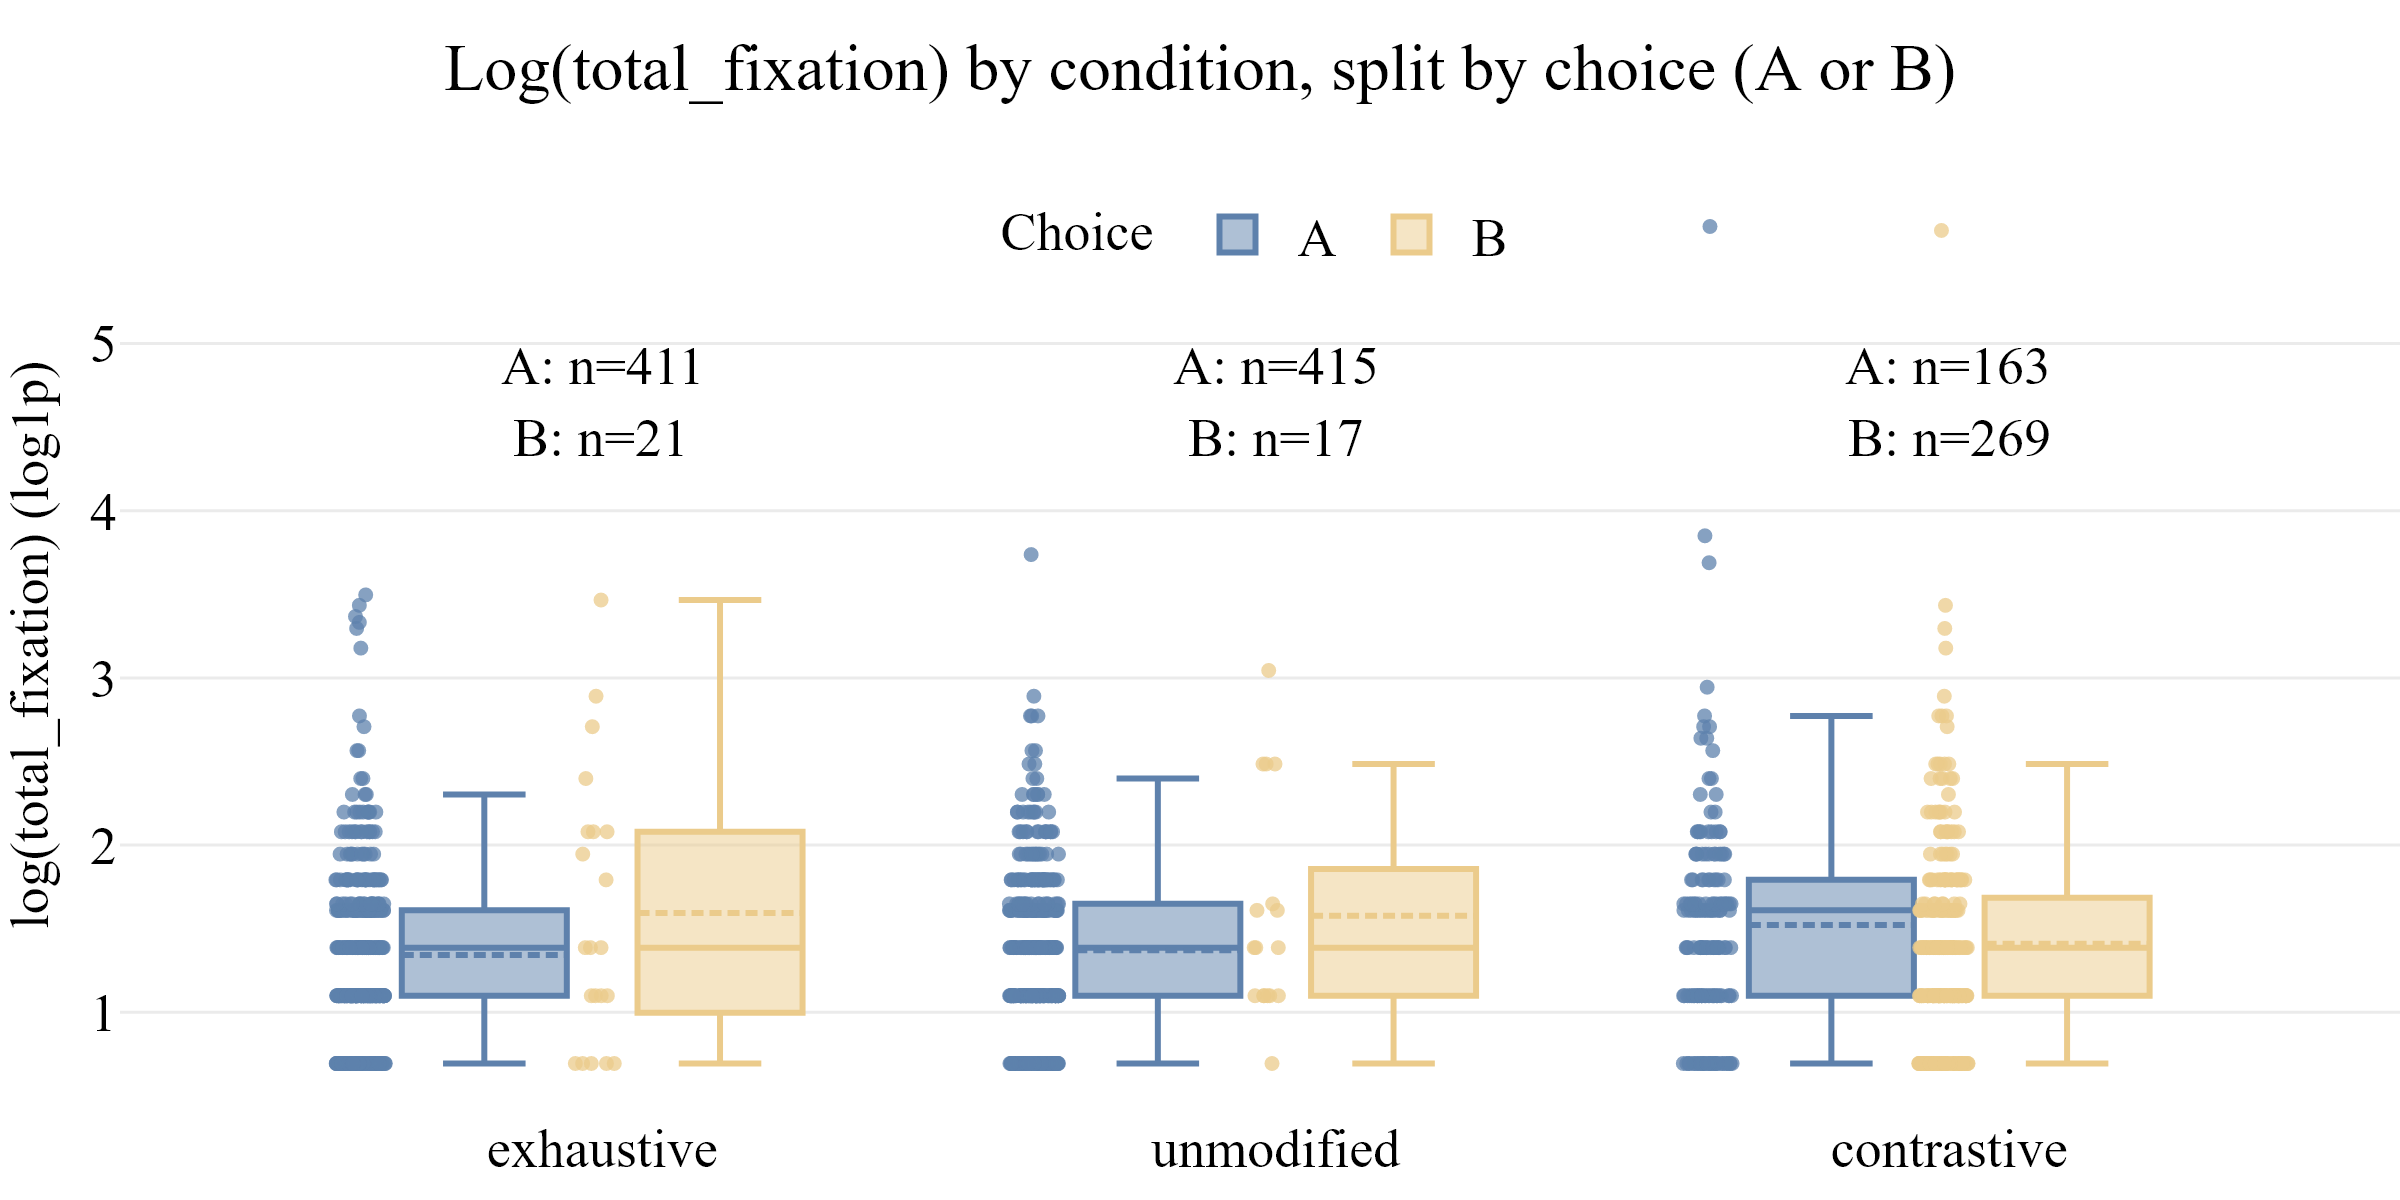
\includegraphics[width=1.0\textwidth]{figs/log_total_fixation_by_condition_and_choice.png}}
{\caption{Total fixation count (log-transformed) by condition and choice type}}
\label{fig:fixation}
\end{figure}



\begin{table}[htbp]
\centering
\caption{Type III Wald chi-square tests for total fixation times}
\label{tab:total-fixation}
\begin{tabularx}{\textwidth}{@{}Xrrr@{}}
\toprule
Effect & $\chi^2$ & df & $p$ \\
\midrule
Condition & 12.33 & 2 & .002 \\
Chosen type & 3.35 & 1 & .067 \\
Condition $\times$ Chosen type & 6.76 & 2 & .034 \\
\bottomrule
\end{tabularx}
\end{table}

\begin{table}[htbp]
\centering
\caption{Fixed effects for total fixation times}
\label{tab:total-fixation-fixed}
\begin{tabularx}{\textwidth}{@{}Xrrrr@{}}
\toprule
Effect & Estimate & SE & df & $p$ \\
\midrule
Intercept & 1.34642 & 0.05092 & 69.60 & $< .001$ \\
Condition (unmodified) & 0.02654 & 0.03208 & 1208.20 & .408 \\
Condition (contrastive) & 0.15751 & 0.04525 & 1252.55 & $< .001$ \\
Choice B & 0.20164 & 0.11023 & 1254.25 & .068 \\
Condition (unmodified) $\times$ Choice B & -0.07622 & 0.15967 & 1235.25 & .633 \\
Condition (contrastive) $\times$ Choice B & -0.28643 & 0.12290 & 1265.34 & .020 \\
\bottomrule
\end{tabularx}
\end{table}

For \textit{total fixation count}, the trends were similar but much weaker. The Type III Wald chi-square tests showed a significant main effect of Condition on fixation count, $\chi^2(2)=12.33$, $p=.002$, and a significant Condition $\times$ Choice interaction, $\chi^2(2)=6.76$, $p=.034$, but no significant main effect of Choice, $\chi^2(1)=3.35$, $p=.067$ (see Table~\ref{tab:total-fixation}). Thus, fixation counts varied across conditions, and the effect of condition depended on which image type participants chose.

The fixed-effects model, using the exhaustive condition and Choice A as reference levels, showed that fixation counts were significantly higher in the contrastive condition ($\beta=0.15751$, $SE=0.04525$, $df=1252.55$, $p<.001$), whereas the unmodified condition did not differ from the exhaustive baseline ($\beta=0.02654$, $SE=0.03208$, $df=1208.20$, $p=.408$; see Table~\ref{tab:total-fixation-fixed}). Choice B showed only a marginal effect ($\beta=0.20164$, $SE=0.11023$, $df=1254.25$, $p=.068$). There was no significant interaction between the unmodified condition and Choice B ($\beta=-0.07622$, $SE=0.15967$, $df=1235.25$, $p=.633$), but there was a significant negative interaction between the contrastive condition and Choice B ($\beta=-0.28643$, $SE=0.12290$, $df=1265.34$, $p=.020$), indicating that the increase in fixation count in the contrastive condition was reduced when participants selected Choice B.

\begin{table}[htbp]
\centering
\caption{Tukey-adjusted pairwise comparisons for total fixation times within choice type (A--A and B--B pairs)}
\label{tab:total-fixation-pairwise-within-choice}
\begin{tabularx}{\textwidth}{@{}Xrrrrr@{}}
\toprule
Contrast & Estimate & SE & df & $t$ & $p$ \\
\midrule
Exhaustive A -- Unmodified A   & -0.02654 & 0.0321 & 1213 & -0.826 & .9628 \\
Exhaustive A -- Contrastive A  & -0.15751 & 0.0454 & 1258 & -3.471 & .0071 \\
Unmodified A -- Contrastive A  & -0.13097 & 0.0452 & 1256 & -2.898 & .0441 \\
Exhaustive B -- Unmodified B   &  0.04968 & 0.1560 & 1239 &  0.318 & .9996 \\
Exhaustive B -- Contrastive B  &  0.12892 & 0.1120 & 1260 &  1.151 & .8596 \\
Unmodified B -- Contrastive B  &  0.07924 & 0.1220 & 1249 &  0.652 & .9869 \\
\bottomrule
\end{tabularx}
\end{table}

\begin{table}[htbp]
\centering
\caption{Tukey-adjusted pairwise comparisons for total fixation times across choice type (A--B pairs)}
\label{tab:total-fixation-pairwise-across-choice}
\begin{tabularx}{\textwidth}{@{}Xrrrrr@{}}
\toprule
Contrast & Estimate & SE & df & $t$ & $p$ \\
\midrule
Exhaustive A -- Exhaustive B   & -0.20164 & 0.1110 & 1259 & -1.824 & .4507 \\
Unmodified A -- Unmodified B   & -0.12542 & 0.1210 & 1252 & -1.038 & .9051 \\
Contrastive A -- Contrastive B &  0.08479 & 0.0517 & 1284 &  1.640 & .5718 \\
\bottomrule
\end{tabularx}
\end{table}

The post-hoc comparisons within choice type showed that for Choice A, fixation counts were significantly lower in the exhaustive condition than in the contrastive condition ($\beta=-0.15751$, $p=.0071$), and also lower in the unmodified condition than in the contrastive condition ($\beta=-0.13097$, $t=-2.898$, $p=.0441$). By contrast, exhaustive and unmodified Choice A trials did not differ significantly ($p=.9628$). For Choice B, none of the condition contrasts reached significance (all $p \ge .8596$), indicating that the condition effect was driven primarily by trials in which participants selected Choice A.

The across-choice comparisons showed no significant difference between Choice A and Choice B within any single condition: exhaustive A vs.\ exhaustive B was not significant ($\beta=-0.20164$, $p=.4507$), nor were unmodified A vs.\ unmodified B ($p=.9051$) and contrastive A vs.\ contrastive B ($p=.5718$). Taken together, these post-hoc results suggest that the interaction observed in reflects differences across conditions for Choice A, rather than robust within-condition differences between Choice A and Choice B.

% Together with the behavioural choice pattern, these results suggest a robust exhaustive bias for PVF when no additional contrastive licensing is present, and increased processing cost when an exhaustive (type A) choice is made in a contrastive context.






\section{Discussion}
\label{sec:discussion}

\subsection{Overview}

The central question of this study was whether the Hungarian pre-verbal focus (PVF) construction inherently encodes exhaustivity, or whether exhaustive and contrastive readings are both available, arising from different pragmatic inferences. Our results, drawn from behavioural choice data, self-paced reading times, and webcam-based eye tracking, converge on a consistent picture: the PVF construction carries a strong but cancellable exhaustive bias. This bias is not semantically obligatory, but it is robust -- strong enough to persist even in the presence of an explicit contrastive licensing phrase. The following sections discuss the implications of each converging line of evidence, and then situate these findings within the broader theoretical debate and prior experimental literature.



\subsection{The exhaustive bias of the unmodified PVF construction}

The most striking finding from the behavioural data is perhaps also the most expected one, yet it has not been demonstrated this directly before: unmodified PVF sentences pattern almost identically with explicitly exhaustive \textit{csak} `only'-sentences in terms of choice behaviour. Participants chose the single-object, exhaustive interpretation in 95.1\% of exhaustive trials and in 96.1\% of unmodified PVF trials (see Table~\ref{tab:choice}), with no significant difference between the two. This near-ceiling alignment is striking and helps explain the intuition that motivated the original claim by \citet{ekiss_1998_identificational} and later by \citet{szabolcsi_1981_compositionality} and \citet{kenesei_2006_focus} that the PVF position is inherently exhaustive: for everyday, out-of-context sentences, the exhaustive reading is overwhelmingly dominant, and it is understandable why this was originally taken to be a semantic, rather than pragmatic, property.

However, the similarity in choice rates between the exhaustive and unmodified conditions does not mean these two conditions were processed identically. The reading time data reveals a qualitative difference: exhaustive sentences were read significantly faster than unmodified PVF sentences at the sentence level ($p < .001$), and at each of the critical regions -- the modifier/focus region (r5, $p = .0003$), the focused object (r6, $p = .018$), and the sentence-final verb (r7, $p < .0001$). This processing advantage was consistently observed in trials where participants ultimately selected the expected single-object image (Choice A), but not in multi-object choice trials, suggesting that the facilitation was tied to the alignment between the explicit exhaustive reading and the chosen interpretation, rather than to the exhaustive marker \textit{csak} per se.

This pattern is consistent with an account in which explicitly marked exhaustivity (\textit{csak} `only') provides an early, unambiguous cue that guides comprehension, allowing readers to resolve the sentence meaning faster and with less processing cost. In contrast, an unmodified PVF sentence leaves the degree of exclusivity initially underspecified, requiring the reader to derive the exhaustive interpretation via pragmatic inference -- and this inferential step comes at a measurable processing cost. This interpretation aligns directly with \citet{balogh_2013_hungarian}'s proposal that exhaustivity in the PVF is not due to a covert exhaustivity operator, but is derived as a pragmatic implicature, similarly to how scalar inferences arise in the broader experimental pragmatics literature \citep[cf.][]{kaldi_2018_linguistic}. The analogy with scalar implicature computation is theoretically informative: just as the inference from `some' to `not all' is computed later and more effortfully than a lexically specified quantifier \citep[cf.][]{kaldi_2021_hungarian_structural}, the exhaustive reading of a bare PVF sentence appears to require an additional inferential step compared to the sentence with \textit{csak}.



\subsection{Contrastive readings: available but costly}

The contrastive condition reveals the complementary side of this picture. When the PVF was modified with \textit{többek között} `amongst others' -- a phrase with inherently inclusive, non-exhaustive meaning -- participants switched to preferring the multi-object, contrastive interpretation in 62.3\% of trials, a dramatic shift from the near-floor level of B-choices in the other two conditions (4.86\% and 3.94\% respectively; see Table~\ref{tab:choice} and Figure~\ref{fig:choice}). This clearly demonstrates that a contrastive, non-exhaustive reading of the PVF construction is not only theoretically possible but is genuinely available to speakers and can be readily elicited. This is an important empirical finding, corroborating the theoretical positions of \citet{wedgwood_2006_hungarian}, \citet{onea_2009_hungarian}, \citet{balogh_2013_hungarian}, and \citet{kaldi_2016_magyar}, who all challenged the view that PVF obligatorily encodes exhaustivity.

Notably, however, the contrastive reading did not dominate the contrastive condition either: 37.7\% of choices in this condition were still the single-object, exhaustive image. This is a significant proportion. Even when the sentence explicitly licences a non-exhaustive reading with a contrastive modifier, the association between the PVF construction and exhaustive interpretation is strong enough to persist at non-trivial levels. The fact that exhaustivity is `cancellable' in the formal, pragmatic sense -- as shown by the grammaticality of sentences such as (\ref{ex:amongst_others}) -- does not mean that cancellation is cognitively effortless. These results suggest that the exhaustive bias associated with PVF is deeply entrenched in speakers' representations of this construction, such that even an explicit licensing phrase does not fully override it.

This finding is further corroborated by the reaction time and eye-tracking data for the contrastive condition. Decision reaction times were significantly longer in the contrastive condition than in the exhaustive condition ($p = .040$), and -- crucially -- participants who ultimately chose the single-object image (A) in the contrastive condition spent significantly more time looking at the images before deciding than participants in the exhaustive condition ($\hat\beta = 0.1876$, $p = .0057$, Table~\ref{tab:total-dwell-pairwise-within-choice}). Choosing an exhaustive image after reading a sentence that grammatically licences a non-exhaustive reading is thus a cognitively costly act -- one that requires overcoming the pragmatic push of \textit{többek között}. Similarly, fixation counts for Choice A were significantly higher in the contrastive than in either the exhaustive ($p = .0071$) or unmodified ($p = .0441$) conditions. Together, these results are consistent with the idea that committing to the exhaustive interpretation in a contrastive context requires additional deliberation, reflecting the competition between the PVF's default exhaustive bias and the non-exhaustive semantics of the modifier.



\subsection{The unmodified PVF as semantically underspecified}

Perhaps the most theoretically significant result from the eye-tracking analysis is the absence of a significant difference in total dwell time between Choice A and Choice B in the \textit{unmodified} condition ($\hat\beta = -0.2390$, $p = .539$; see Table~\ref{tab:total-dwell-pairwise-across-choice}). This stands in stark contrast to the exhaustive condition, where participants dwelled significantly less on the images when selecting the expected exhaustive (A) choice ($\hat\beta = -0.4443$, $p = .0081$), reflecting the ease and clarity of the exhaustive decision. In the unmodified condition, however, participants showed no significant asymmetry in how long they looked before choosing A or B. This null result is informative: it suggests that, during the actual moment of decision, both the exhaustive and contrastive interpretations were equally plausible to participants when the PVF was used without any modifying marker.

This pattern of results is consistent with a model of semantic underspecification \citep[cf.][]{wedgwood_2006_hungarian}, in which the unmodified PVF does not lexically or structurally fix the degree of exhaustivity, leaving this to be resolved by contextual and pragmatic factors. The strong behavioural preference for single-object images (96.1\% Choice A) reflects a default pragmatic bias -- a prior expectation that PVF sentences are exhaustive in the absence of other information -- but the eye-tracking data suggests that this default is not so deeply entrenched as to make the contrastive reading cognitively inaccessible. In other words, the majority of participants converge on the exhaustive reading, but those who entertained the contrastive reading did so without appreciably greater cognitive effort. The PVF, in isolation, is thus best characterised not as a semantic exhaustivity operator, but as a pragmatically enriched construction with a strong, context-sensitive exhaustive default.

This result reconciles what initially appear to be contradictory observations in the literature. The received view \citep{szabolcsi_1981_compositionality,ekiss_1998_identificational,kenesei_2006_focus,horvath_2008_separating} is motivated by the near-universal intuition that PVF sentences entail exhaustivity -- which our data confirms. But the conclusion that this entailment is semantic rather than pragmatic was based on intuitions and theoretical argument, not on direct evidence about the availability of non-exhaustive readings. Our results, along with the earlier experimental work by \citet{onea_2009_hungarian}, \citet{gerocs_2014_exhaustivity}, and \citet{kaldi_2018_linguistic}, provide such evidence, and it consistently points toward a pragmatic analysis.



\subsection{Relation to prior experimental work}

Our findings converge with and extend a growing body of experimental literature on Hungarian focus exhaustivity. \citet{onea_2009_hungarian} were among the first to provide experimental evidence that the Hungarian PVF is not semantically exhaustive, showing that exhaustivity effects are stronger in the presence of verbal particles (and thus cannot be attributed to focus position alone), and proposing a pragmatic analysis grounded in question-answering. Our results are fully consistent with their core claim and add direct evidence from a richer set of dependent measures -- not only behavioural choices, but also reading times and eye movements -- that allow us to characterise the temporal dynamics and cognitive cost of exhaustive and contrastive interpretations.

\citet{gerocs_2014_exhaustivity} provided further experimental evidence using an offline task paradigm, showing that exhaustive interpretation of the PVF is not obligatory and can be contextually modulated. Our study extends this with an online, time-sensitive paradigm that tracks both reading and gaze, thereby providing a window into the comprehension process rather than just its endpoint. The directional pattern in our data aligns with theirs: unmodified PVF is exhaustive by default, but not obligatorily so.

Most directly comparable to the current study is \citet{kaldi_2018_linguistic}, who used a visual-world eye-tracking paradigm to investigate how context (restrictive vs.\ non-restrictive) modulates the exhaustive inference associated with Hungarian PVF. Their central finding was that the rate of exhaustive interpretation was context-dependent, supporting a pragmatic/implicature account of PVF exhaustivity. Our study complements this by removing context manipulation and instead comparing conditions that explicitly force or cancel exhaustivity against an unmodified baseline, making it possible to characterise the strength and resilience of the exhaustive default. The null A--B dwell difference in our unmodified condition, together with the strong choice preference for A, mirrors the picture \citeauthor{kaldi_2018_linguistic} describe: PVF creates a strong exhaustive tendency, but this tendency is sensitive to linguistic input and is not a hard semantic entailment. \citet{kaldi_2021_hungarian_preverbal}'s doctoral work situating exhaustivity as a scalar type implicature provides a natural theoretical home for these empirical patterns: like other scalar inferences, the exhaustive reading is the pragmatically expected default, but can be computed more slowly than lexically specified exclusivity and is cancellable by appropriate context or explicit licensing.

Our findings also invite a cross-linguistic perspective. \citet{hsu_2019_associations} investigated the association between focus constructions and exhaustivity in Chinese, comparing wh-focus, cleft-focus, and \textit{only}-focus using a trichotomous-response design. Their results showed that cleft-focus and only-focus were clearly distinguished from wh-focus in terms of exhaustivity associations, with both triggering robust exhaustive readings, while still differing subtly from each other in conscious decision-making tasks. The structurally different mechanism of Hungarian PVF -- syntactic fronting and eradicating prosodic stress, as opposed to a cleft construction -- nonetheless leads to a broadly similar functional outcome: a construction that strongly associates with exhaustivity without necessarily encoding it as a semantic entailment. This parallel across typologically distinct languages is consistent with the view that exhaustive readings of grammaticalized focus constructions arise through a common pragmatic mechanism, rather than through a language-specific semantic operator, a point also raised by \citet{krifka_2008_basic} in his account of information structure subtypes.



\subsection{Theoretical implications}

Taken together, our results have clear implications for the theoretical debate on the semantics and pragmatics of Hungarian PVF. The strong semantic exhaustivity view -- that an immediately pre-verbal focused constituent is semantically exhaustive, i.e.\ it is true that no other entity satisfies the predicate \citep{szabolcsi_1981_compositionality,ekiss_1998_identificational,ekiss_2007_topic,kenesei_2006_focus,horvath_2008_separating} -- predicts that (i) non-exhaustive readings should be unavailable or highly marked, (ii) the unmodified PVF should be processed identically to the \textit{only}-condition, and (iii) co-occurrence with \textit{többek között} `amongst others' should be degraded or induce a strong semantic conflict. None of these predictions is borne out. Non-exhaustive readings were chosen in over a third of contrastive trials, the unmodified condition was processed more slowly than the explicitly marked exhaustive condition, and the contrastive condition was grammatically acceptable and produced meaningful, interpretable results.

In contrast, the pragmatic exhaustivity view -- most fully developed for Hungarian by \citet{balogh_2013_hungarian} in the tradition of \citet{rooth_1992_theory}'s alternative semantics and \citet{vallduvi_1998_rheme}'s notion of \textit{kontrast} -- predicts that (i) the exhaustive reading is the default inference but can be cancelled, (ii) the lexical exhaustivity marker provides a shorter, more direct path to the exhaustive interpretation, and (iii) cancellation of the exhaustive reading (via \textit{többek között}) is possible but comes at a processing cost, given the competing default. All three of these predictions are supported by our data. \citet{zimmermann_2008_contrastive}'s view that contrastivity is a pragmatic, discourse-structuring phenomenon, rather than a semantic property, is also consistent: the PVF does not select between exhaustive and contrastive readings at the semantic level; instead, this is a discourse-level resolution that depends on context, prior beliefs, and the presence of additional cues.

In \citeauthor{ekiss_1998_identificational}'s (\citeyear{ekiss_1998_identificational}) framework, both exhaustive and contrastive readings fall under \textit{identificational focus}, defined as a focus that identifies a referent from a set of alternatives, described as [+exhaustive] and optionally [+contrastive]. Our results challenge the claim that such focus is inherently [+exhaustive] as a semantic entailment, while being compatible with the weaker claim that exhaustivity is the prototypical inferential outcome of identificational focus. Indeed, the very near-ceiling exhaustive choices for the unmodified PVF (96.1\%) show that the pragmatic bias towards exhaustivity is extremely strong -- strong enough to look, at first, like a semantic entailment -- but the eye-tracking evidence of equal decision effort for A and B choices in this condition reveals that the construction leaves the exhaustivity question genuinely open.

It is also worth connecting these results to \citeauthor{gecseg_2020_focused}'s (\citeyear{gecseg_2020_focused}) observation that focused topics in Hungarian show discourse-configurational prominence without necessarily encoding exhaustivity, and to \citet{genzel_2015_prosodic}'s finding that prosodic expression in Hungarian focus constructions varies as a function of the type of focus (narrow, broad, contrastive). These latter results suggest that even at the phonological level, the PVF construction is not a monolithic exhaustivity trigger; the same syntactic position can host focus with distinct prosodic, semantic, and pragmatic profiles. Our results add the comprehension dimension to this picture, showing that the same surface form -- the unmodified PVF -- is genuinely compatible with more than one interpretive outcome.



\subsection{Limitations and future directions}

Several limitations of the current study deserve acknowledgement. First, our eye-tracking data was collected via webcam using the WebGazer.js library integrated into PCIbex, which, while enabling large-scale online data collection, has substantially lower spatial and temporal precision than laboratory-based eye-tracking systems. Gaze was classified into two broad areas of interest (left and right canvases), collapsing the rich spatio-temporal information available in high-resolution systems. Our episode-based cleaning procedure addressed some artefacts of this method, but absolute magnitudes of dwell time and fixation count should be interpreted cautiously, and the null effects we report (particularly in the unmodified condition) should be understood in the context of this reduced precision. Nonetheless, the consistency between the dwell time and fixation count results, and their alignment with the reading time and behavioural patterns, strengthens confidence in the key contrasts.

Second, the forced-choice, sentence--picture verification paradigm we used requires participants to commit to one of two interpretations and does not capture gradient or intermediate representations. The 37.7\% exhaustive choices in the contrastive condition, for example, could reflect either genuine exhaustive interpretations or a residual structural bias that the paradigm forces into a categorical outcome. Future work using magnitude estimation, acceptability rating, or more fine-grained response measures could help disentangle these possibilities.

Third, the contrastive condition employed a single licensing phrase, \textit{többek között} `amongst others'. It remains an open question whether other contrastive devices -- additive particles, correction contexts, or naturally occurring discourse embedding -- would produce the same degree of exhaustivity suppression or a different pattern. The robustness of the exhaustive default across different contrastive contexts is an empirically open question that deserves further investigation.

Fourth, as an online study with participant-owned devices, there was considerable variability in the technical quality of the eye-tracking data. A substantial proportion of participants could not pass the calibration threshold and were thus excluded before the experiment began. This raises a self-selection concern: participants who successfully calibrated may not be fully representative of the broader population of Hungarian speakers, potentially skewing the sample toward those with higher-resolution webcams, better lighting, or greater attentiveness to technical instructions.

Future research could address these limitations in several ways. A laboratory-based replication with high-resolution remote eye-tracking would allow more precise characterisation of the gaze dynamics, including measures such as first-fixation latency, proportion of looks over time, and fixation duration distributions. The use of context-embedded stimuli -- placing the target PVF sentence in a prior discourse that either restricts or expands the relevant set of alternatives -- would allow a more direct comparison with \citet{kaldi_2018_linguistic}'s context-dependent exhaustivity paradigm. Production experiments could complement the comprehension data by examining which conditions prompt speakers to spontaneously add exhaustive or contrastive modifiers to an otherwise bare PVF. Finally, a systematic cross-linguistic investigation using the same paradigm for other languages with grammaticalized focus constructions \citep[cf.][]{hsu_2019_associations,cruschina_2021_greater} would allow researchers to test whether the strong-but-cancellable exhaustive bias is a universal property of syntactically marked identificational focus, or a Hungarian-specific effect shaped by the language's particular discourse-configurational grammar \citep{ekiss_1995_discourse}.

Besides this, it would be interesting to investigate whether specific features of Hungarian have any effect on the interpretation of focus constructions, such the definiteness--indefiniteness of the objects and the use of the definite conjugation, the countability--uncountabulity of the objects, the presence of verbal prefixes, the aspect of the verbs, and the tense of the verbs (past vs present).  



\section{Conclusion}
\label{sec:conclusion}

This study investigated the interpretation and processing of Hungarian pre-verbal focus (PVF) constructions using a sentence--picture verification task with self-paced reading and webcam-based eye tracking. Our central empirical question was whether the PVF construction inherently encodes exhaustivity, or whether both exhaustive and contrastive, non-exclusive readings are genuinely available to Hungarian speakers. The results provide a clear and consistent answer: the PVF construction does not independently encode exhaustivity, but it carries a strong and robust default bias towards exhaustive interpretation.

Behaviourally, unmodified PVF sentences were interpreted exhaustively in over 96\% of trials -- virtually identically to sentences with the explicit exhaustive marker \textit{csak} `only' -- demonstrating that the exhaustive reading is the overwhelming default in the absence of contextual information. This confirms the intuition behind the classical semantic accounts \citep{szabolcsi_1981_compositionality,ekiss_1998_identificational,kenesei_2006_focus}. However, it does not vindicate the stronger semantic claim: when the PVF was modified with \textit{többek között} `amongst others', a phrase that licences a non-exhaustive, contrastive reading, participants shifted to preferring the multi-object image in 62.3\% of trials, clearly showing that the exhaustive reading is cancellable and that a contrastive interpretation is genuinely available. The exhaustivity bias persisted even here -- roughly a third of contrastive-condition choices were still exhaustive -- but it was substantially weakened.

The processing data add an important dimension that the behavioural choices alone cannot reveal. Reading times were fastest for the explicitly exhaustive condition at every critical region, reflecting the processing efficiency of a lexically specified, unambiguous exhaustivity cue. The unmodified PVF was read more slowly, consistent with the view that exhaustivity must be inferred pragmatically rather than read off directly from the semantics of the construction. Most tellingly, eye-tracking data showed that participants deliberated equally long before choosing an exhaustive or contrastive image for unmodified PVF sentences -- a null result that is informative: it suggests that both readings remained equally plausible at the point of decision. In contrast, exhaustive-condition choices were made faster and with less hesitation, and contrastive-condition choices for the unexpected exhaustive image required significantly more deliberation and more looks at the images.

Taken together, these findings support the view that PVF exhaustivity arises not from a covert semantic operator or structural feature, but from a pragmatic inference -- a strong but contextually sensitive default that can be manipulated, cancelled, and bears a measurable processing cost when overridden. This positions the current study alongside and in support of the growing experimental literature challenging the semantic exhaustivity view \citep{onea_2009_hungarian,gerocs_2014_exhaustivity,kaldi_2018_linguistic,kaldi_2021_hungarian_preverbal}, and provides the most direct online psycholinguistic evidence to date that the Hungarian PVF construction is semantically underspecified with respect to exhaustivity.

More broadly, these results demonstrate that the long-standing theoretical controversy about whether PVF exhaustivity is semantic or pragmatic can and should be resolved through psycholinguistic experimentation. The parallel processing cost profiles for pragmatic inference -- slower reading, greater deliberation, more effortful decisions -- converge with what experimental pragmatics has established for scalar implicatures more generally \citep[cf.][]{kaldi_2021_hungarian_structural}, supporting a unified account in which exhaustive readings of PVF sentences are a species of pragmatic enrichment, not truth-conditional content. The construction is, in a meaningful sense, ambiguous -- or at least underspecified -- and Hungarian speakers navigate this underspecification fluidly, defaulting to exhaustivity but remaining sensitive to linguistic cues that license contrastive alternatives.



\section{NOTES}

\hl{Notes and todo lists go here.}

\subsection{Todo list}
\begin{itemize}
   \item Check Results section once again.
   \item Check Discussion and Conclusion.
   \item Check journal rules about Appendix
\end{itemize}



\begin{Backmatter}

\paragraph{Acknowledgments}
The authors also wish to thank ... \hl{if any}.

\paragraph{Funding statement}
This study was funded by ... \hl{if any}.

\paragraph{Data availability statement} \label{sec:data-statement}
Stimuli, full results, replication data and code can be found at \url{https://osf.io/j9abg/overview?view_only=484a4f21a5cb4e51b4b826f970e096a0}.

\clearpage

\section*{Appendix}

% Full-page grid of all stimuli (18 pairs = 36 images).
% Layout: 4 images per row (two A/B pairs), 9 rows total.
\begin{figure*}[!ht]
\centering
% Tighten the grid spacing
\setlength{\tabcolsep}{1pt} % horizontal padding between columns
\renewcommand{\arraystretch}{0.5} % reduce extra vertical padding in tabular rows
\FIG{
\begin{tabular}{@{}rcc@{\hspace{20pt}}rcc@{}}
\# & A & B & \# & A & B \\
1 & 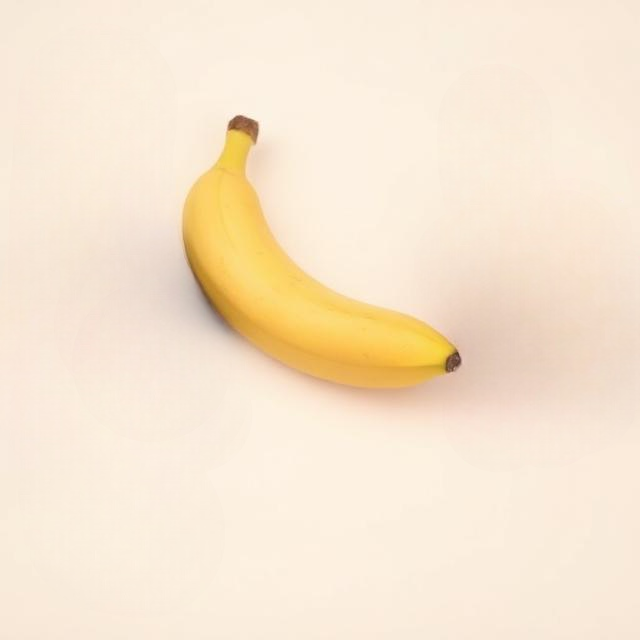
\includegraphics[height=.096\textheight]{figs/1a.png}  &
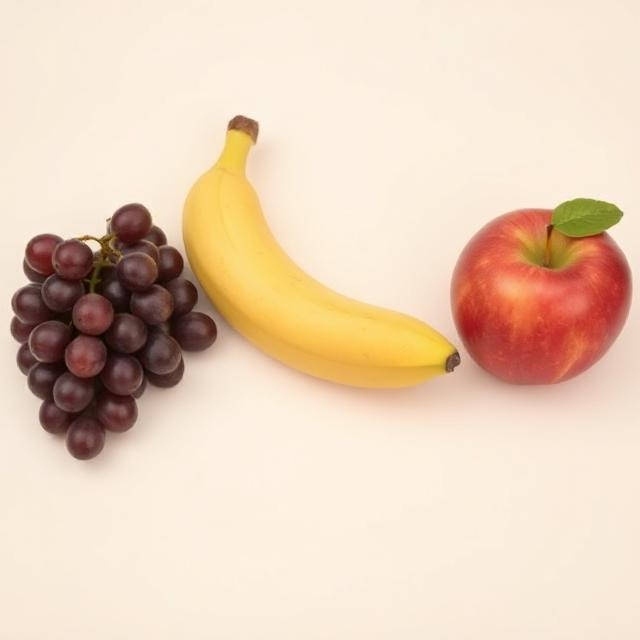
\includegraphics[height=.096\textheight]{figs/1b.png}  &
2 & 
\includegraphics[height=.096\textheight]{figs/2a.png}  &

\includegraphics[height=.096\textheight]{figs/2b.png}  \\
3 &
\includegraphics[height=.096\textheight]{figs/3a.png}  &

\includegraphics[height=.096\textheight]{figs/3b.png}  &
4 & 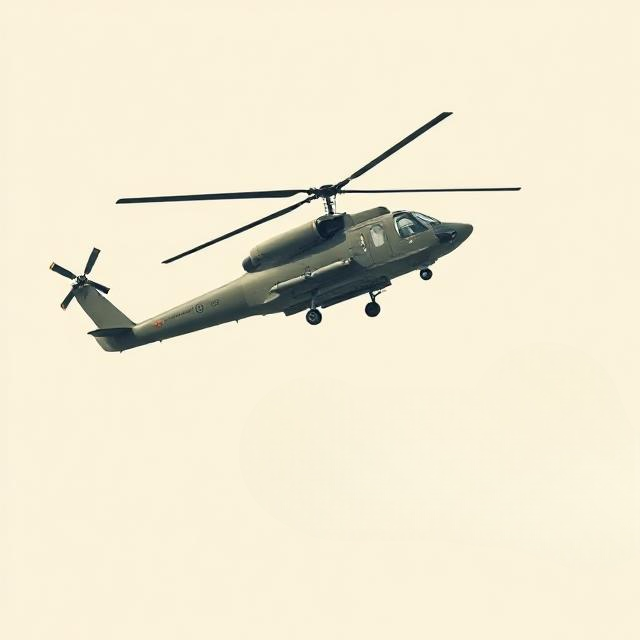
\includegraphics[height=.096\textheight]{figs/4a.png}  &
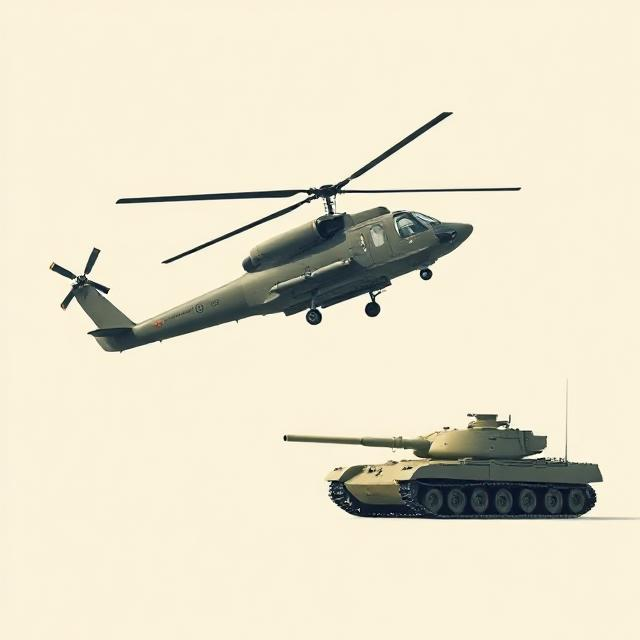
\includegraphics[height=.096\textheight]{figs/4b.png}  \\
5 & 
\includegraphics[height=.096\textheight]{figs/5a.png}  &
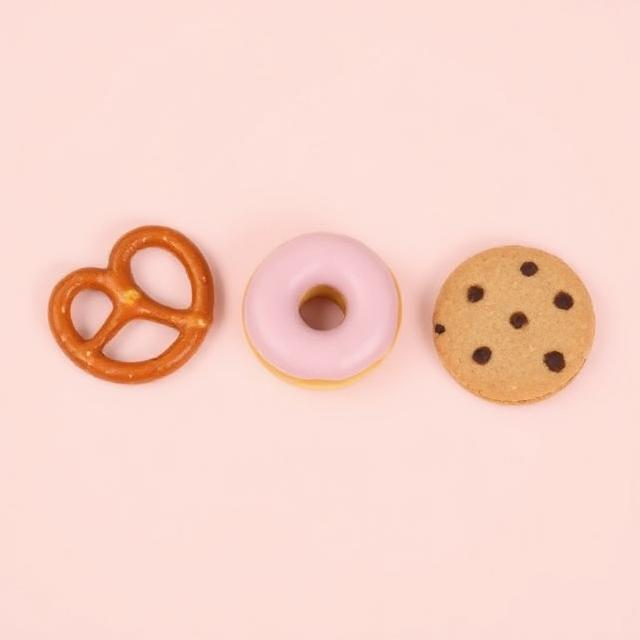
\includegraphics[height=.096\textheight]{figs/5b.png}  &
6 & 
\includegraphics[height=.096\textheight]{figs/6a.png}  &

\includegraphics[height=.096\textheight]{figs/6b.png}  \\
7 & 
\includegraphics[height=.096\textheight]{figs/7a.png}  &

\includegraphics[height=.096\textheight]{figs/7b.png}  &
8 & 
\includegraphics[height=.096\textheight]{figs/8a.png}  &

\includegraphics[height=.096\textheight]{figs/8b.png}  \\
9 & 
\includegraphics[height=.096\textheight]{figs/9a.png}  &

\includegraphics[height=.096\textheight]{figs/9b.png}  &
10 & 
\includegraphics[height=.096\textheight]{figs/10a.png} &
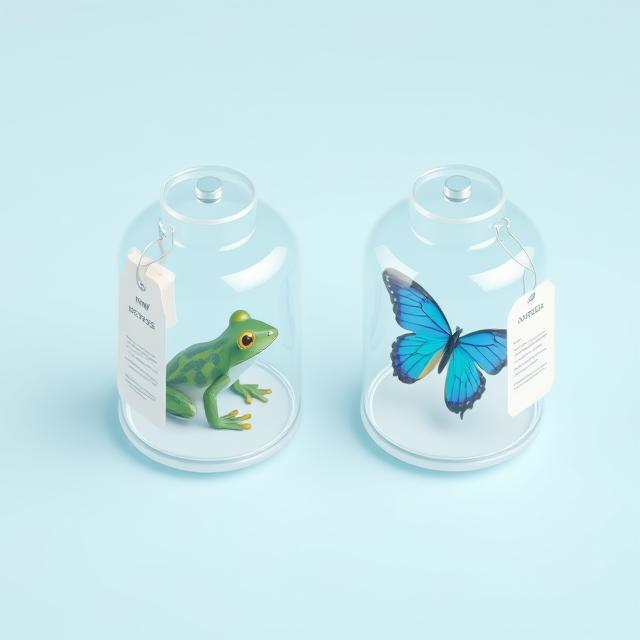
\includegraphics[height=.096\textheight]{figs/10b.png} \\
11 & 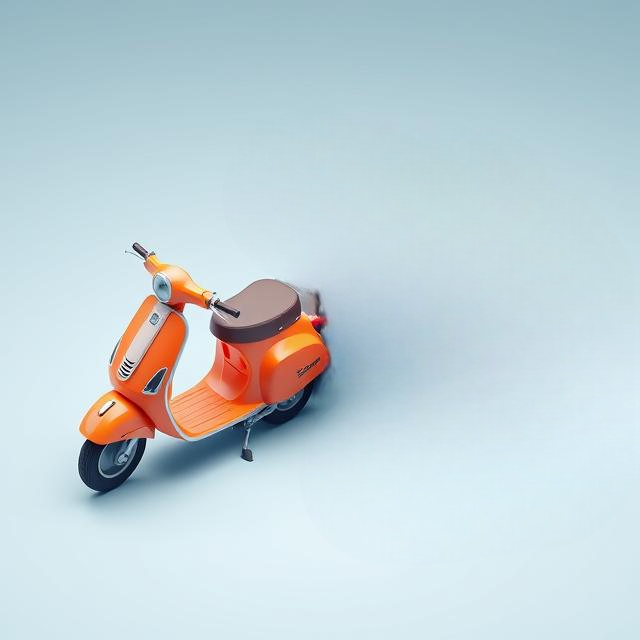
\includegraphics[height=.096\textheight]{figs/11a.png} &

\includegraphics[height=.096\textheight]{figs/11b.png} &
12 & 
\includegraphics[height=.096\textheight]{figs/12a.png} &

\includegraphics[height=.096\textheight]{figs/12b.png} \\
13 & 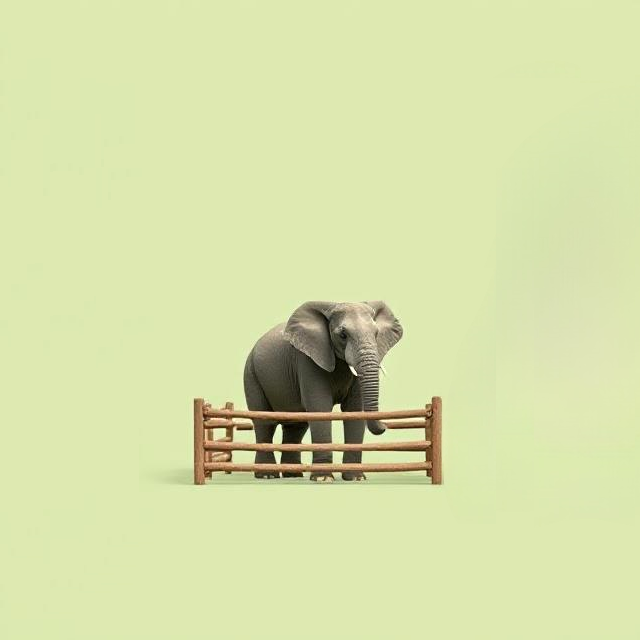
\includegraphics[height=.096\textheight]{figs/13a.png} &
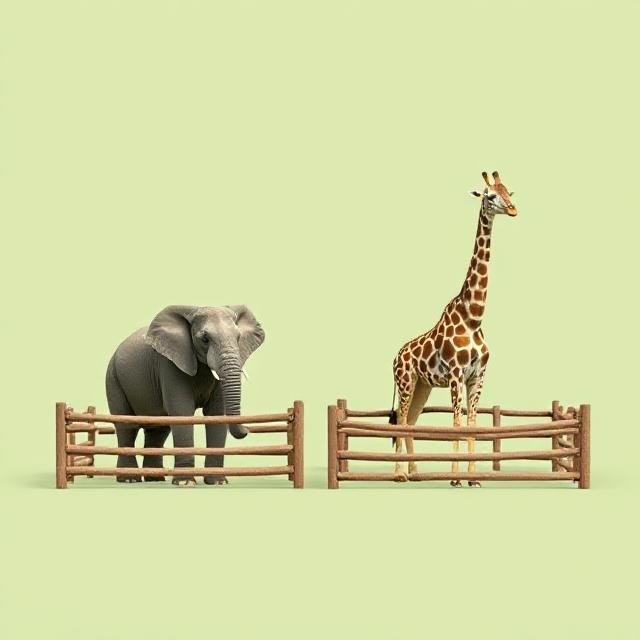
\includegraphics[height=.096\textheight]{figs/13b.png} &
14 & 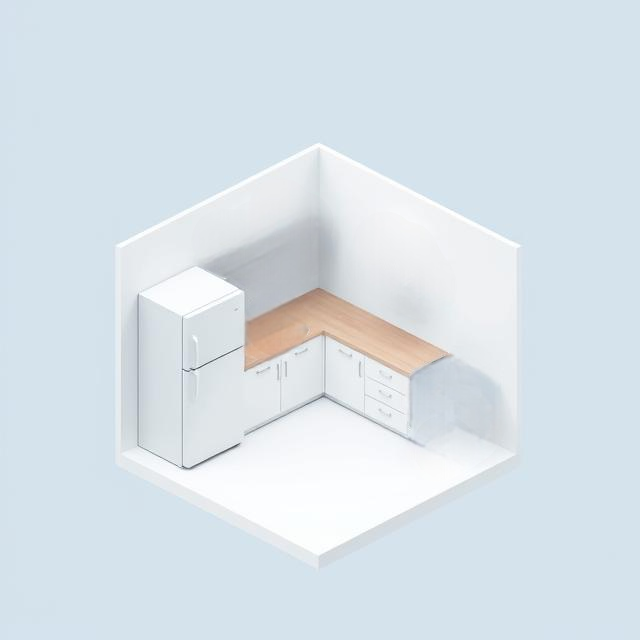
\includegraphics[height=.096\textheight]{figs/14a.png} &
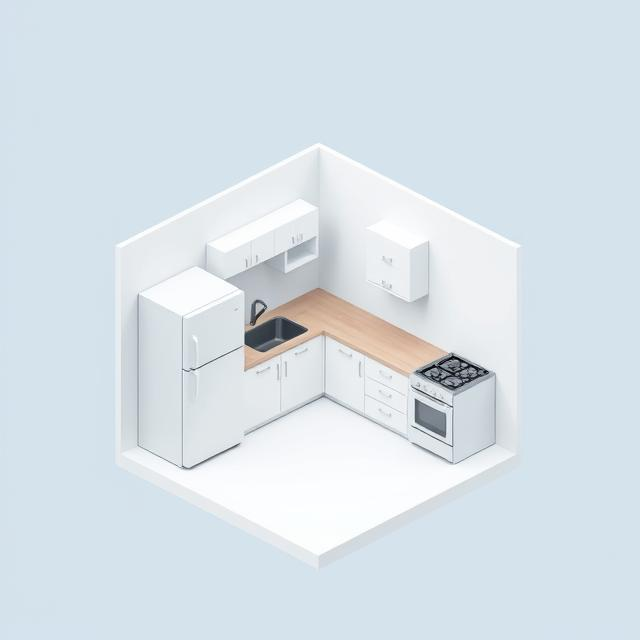
\includegraphics[height=.096\textheight]{figs/14b.png} \\
15 & 
\includegraphics[height=.096\textheight]{figs/15a.png} &

\includegraphics[height=.096\textheight]{figs/15b.png} &
16 & 
\includegraphics[height=.096\textheight]{figs/16a.png} &

\includegraphics[height=.096\textheight]{figs/16b.png} \\
17 & 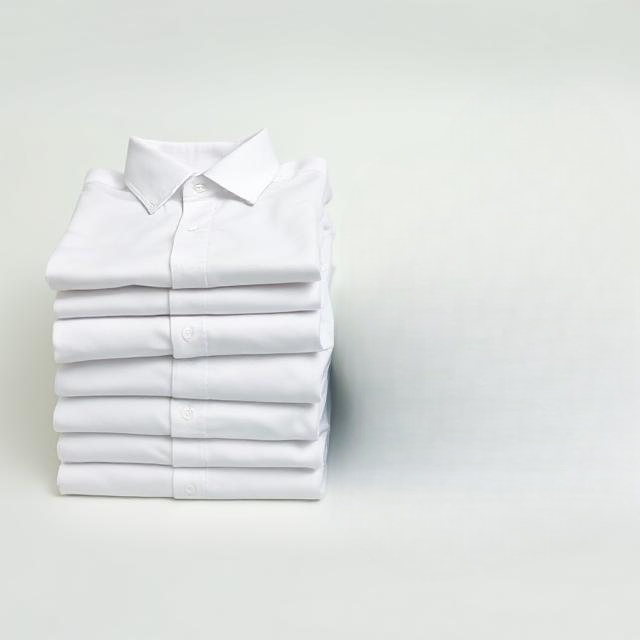
\includegraphics[height=.096\textheight]{figs/17a.png} &
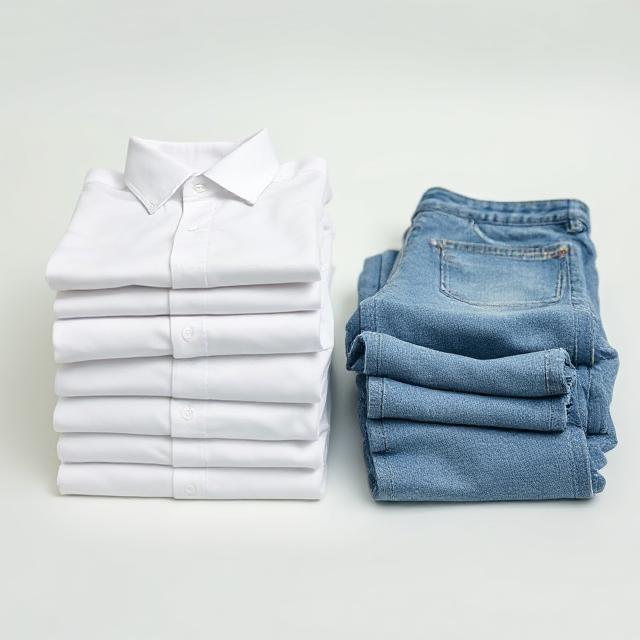
\includegraphics[height=.096\textheight]{figs/17b.png} &
18 & 
\includegraphics[height=.096\textheight]{figs/18a.png} &

\includegraphics[height=.096\textheight]{figs/18b.png} \\
\end{tabular}
}
{\caption{Complete visual stimulus set with A) single- and B) multi-entity image pairs}}
\label{fig:visual_stimuli}
\end{figure*}



% \FloatBarrier
% \Needspace{6\baselineskip}     % ensure enough room, otherwise break before
% \begin{samepage}

\begin{landscape}
\footnotesize
\setlength{\LTleft}{0pt}
\setlength{\LTright}{0pt}
\renewcommand{\arraystretch}{1.05}

\label{tab:sentence_stimuli}
\begin{longtable}{@{}%
r
r
l
>{\raggedright\arraybackslash}p{2.2cm}
>{\raggedright\arraybackslash}p{2.4cm}
>{\raggedright\arraybackslash}p{1.8cm}
>{\raggedright\arraybackslash}p{1.8cm}
>{\raggedright\arraybackslash}p{1.8cm}
>{\raggedright\arraybackslash}p{2.5cm}
>{\raggedright\arraybackslash}p{2.0cm}
@{}}

\caption{Full stimulus list with sentence regions}\label{tab:stimuli-full}\\
\toprule
\textbf{no} & \textbf{item} & \textbf{condition} & \textbf{r1} & \textbf{r2} & \textbf{r3} & \textbf{r4} & \textbf{r5} & \textbf{r6} & \textbf{r7} \\
\midrule
\endfirsthead

\toprule
\textbf{no} & \textbf{item} & \textbf{condition} & \textbf{r1} & \textbf{r2} & \textbf{r3} & \textbf{r4} & \textbf{r5} & \textbf{r6} & \textbf{r7} \\
\midrule
\endhead

\midrule
\multicolumn{10}{r}{Continued on next page}
\endfoot

\bottomrule
\endlastfoot

1 & 1 & exhaustive & \textit{Ami} & \textit{a gyümölcsöket} & \textit{illeti,} & \textit{Anna} & \textit{csak} & \textit{egy banánt} & \textit{evett.} \\
  &   &            & which (relative) & the fruits-ACC & regards & Anna & only & a banana-ACC & ate-3SG \\
  &   &            & \multicolumn{7}{p{16.5cm}@{}}{`Regarding fruits, Anna ate only a banana.'} \\[0.35em]

2 & 1 & unmodified & \textit{Ami} & \textit{a gyümölcsöket} & \textit{illeti,} & \textit{Anna} & \textit{tegnap} & \textit{egy banánt} & \textit{evett.} \\
  &   &            & which (relative) & the fruits-ACC & regards & Anna & yesterday & a banana-ACC & ate-3SG \\
  &   &            & \multicolumn{7}{p{16.5cm}@{}}{`Regarding fruits, Anna ate a banana yesterday.'} \\[0.35em]

3 & 1 & contrastive & \textit{Tegnap} & \textit{reggel} & \textit{Anna} & \textit{többek} & \textit{között} & \textit{egy banánt} & \textit{evett.} \\
  &   &             & yesterday & morning & Anna & others & among & a banana-ACC & ate-3SG \\
  &   &             & \multicolumn{7}{p{16.5cm}@{}}{`Yesterday morning Anna ate, among other things, a banana.'} \\[0.35em]

4 & 2 & exhaustive & \textit{Ami} & \textit{az írószereket} & \textit{illeti,} & \textit{a kisfiú} & \textit{csak} & \textit{egy ceruzát} & \textit{kapott.} \\
  &   &            & which (relative) & the stationeries-ACC & regards & the boy & only & a pencil-ACC & received-3SG \\
  &   &            & \multicolumn{7}{p{16.5cm}@{}}{`Regarding stationery, the boy received only a pencil.'} \\[0.35em]

5 & 2 & unmodified & \textit{Ami} & \textit{az írószereket} & \textit{illeti,} & \textit{a kisfiú} & \textit{tegnap} & \textit{egy ceruzát} & \textit{kapott.} \\
  &   &            & which (relative) & the stationeries-ACC & regards & the boy & yesterday & a pencil-ACC & received-3SG \\
  &   &            & \multicolumn{7}{p{16.5cm}@{}}{`Regarding stationery, the boy received a pencil yesterday.'} \\[0.35em]

6 & 2 & contrastive & \textit{Tegnap} & \textit{reggel} & \textit{a kisfiú} & \textit{többek} & \textit{között} & \textit{egy ceruzát} & \textit{kapott.} \\
  &   &             & yesterday & morning & the boy & others & among & a pencil-ACC & received-3SG \\
  &   &             & \multicolumn{7}{p{16.5cm}@{}}{`Yesterday morning the boy received, among other things, a pencil.'} \\[0.35em]

7 & 3 & exhaustive & \textit{Ami} & \textit{a bútorokat} & \textit{illeti,} & \textit{az asztalos} & \textit{csak} & \textit{egy könyvespolcot} & \textit{készített.} \\
  &   &            & which (relative) & the furniture-ACC & regards & the carpenter & only & a bookshelf-ACC & made-3SG \\
  &   &            & \multicolumn{7}{p{16.5cm}@{}}{`Regarding furniture, the carpenter made only a bookshelf.'} \\[0.35em]

8 & 3 & unmodified & \textit{Ami} & \textit{a bútorokat} & \textit{illeti,} & \textit{az asztalos} & \textit{tegnap} & \textit{egy könyvespolcot} & \textit{készített.} \\
  &   &            & which (relative) & the furniture-ACC & regards & the carpenter & yesterday & a bookshelf-ACC & made-3SG \\
  &   &            & \multicolumn{7}{p{16.5cm}@{}}{`Regarding furniture, the carpenter made a bookshelf yesterday.'} \\[0.35em]

9 & 3 & contrastive & \textit{Tegnap} & \textit{a műhelyben} & \textit{az asztalos} & \textit{többek} & \textit{között} & \textit{egy könyvespolcot} & \textit{készített.} \\
  &   &             & yesterday & in the workshop & the carpenter & others & among & a bookshelf-ACC & made-3SG \\
  &   &             & \multicolumn{7}{p{16.5cm}@{}}{`Yesterday in the workshop the carpenter made, among other things, a bookshelf.'} \\[0.35em]

10 & 4 & exhaustive & \textit{Ami} & \textit{a harci eszközöket} & \textit{illeti,} & \textit{a katonaság} & \textit{csak} & \textit{a helikoptert} & \textit{tesztelte.} \\
   &   &            & which (relative) & the military equipment-ACC & regards & the military & only & the helicopter-ACC & tested-3SG \\
   &   &            & \multicolumn{7}{p{16.5cm}@{}}{`Regarding the equipment, the military only tested the helicopter.'} \\[0.35em]

11 & 4 & unmodified & \textit{Ami} & \textit{a harci eszközöket} & \textit{illeti,} & \textit{a katonaság} & \textit{tavaly} & \textit{a helikoptert} & \textit{tesztelte.} \\
   &   &            & which (relative) & the military equipment-ACC & regards & the military & last year & the helicopter-ACC & tested-3SG \\
   &   &            & \multicolumn{7}{p{16.5cm}@{}}{`Regarding the equipment, the military tested the helicopter this time last year.'} \\[0.35em]

12 & 4 & contrastive & \textit{Tavaly} & \textit{ilyenkor} & \textit{a katonaság} & \textit{többek} & \textit{között} & \textit{a helikoptert} & \textit{tesztelte.} \\
   &   &             & last year & this time & the military & others & among & the helicopter-ACC & tested-3SG \\
   &   &             & \multicolumn{7}{p{16.5cm}@{}}{`This time last year the military tested, among other things, the helicopter.'} \\[0.35em]

13 & 5 & exhaustive & \textit{Ami} & \textit{a süteményeket} & \textit{illeti,} & \textit{én} & \textit{csak} & \textit{a fánkot} & \textit{sütöttem.} \\
   &   &            & which (relative) & the sweets-ACC & regards & I & only & the doughnut-ACC & baked-1SG \\
   &   &            & \multicolumn{7}{p{16.5cm}@{}}{`Regarding the sweets, I only baked the doughnut.'} \\[0.35em]

14 & 5 & unmodified & \textit{Ami} & \textit{a süteményeket} & \textit{illeti,} & \textit{én} & \textit{múltkor} & \textit{a fánkot} & \textit{sütöttem.} \\
   &   &            & which (relative) & the sweets-ACC & regards & I & last time & the doughnut-ACC & baked-1SG \\
   &   &            & \multicolumn{7}{p{16.5cm}@{}}{`Regarding the sweets, I baked the doughnut last time.'} \\[0.35em]

15 & 5 & contrastive & \textit{Tegnap} & \textit{este} & \textit{én} & \textit{többek} & \textit{között} & \textit{a fánkot} & \textit{sütöttem.} \\
   &   &             & yesterday & evening & I & others & among & the doughnut-ACC & baked-1SG \\
   &   &             & \multicolumn{7}{p{16.5cm}@{}}{`Yesterday evening I baked, among other things, a doughnut.'} \\[0.35em]

16 & 6 & exhaustive & \textit{Ami} & \textit{a virágokat} & \textit{illeti,} & \textit{Éva} & \textit{csak} & \textit{a tulipánt} & \textit{szereti.} \\
   &   &            & which (relative) & the flowers-ACC & regards & Eve & only & the tulip-ACC & likes-3SG \\
   &   &            & \multicolumn{7}{p{16.5cm}@{}}{`Regarding flowers, Eve only likes tulips.'} \\[0.35em]

17 & 6 & unmodified & \textit{Ami} & \textit{a virágokat} & \textit{illeti,} & \textit{Éva} & \textit{mostanában} & \textit{a tulipánt} & \textit{szereti.} \\
   &   &            & which (relative) & the flowers-ACC & regards & Eve & nowadays & the tulip-ACC & likes-3SG \\
   &   &            & \multicolumn{7}{p{16.5cm}@{}}{`Regarding flowers, Eve likes tulips nowadays.'} \\[0.35em]

18 & 6 & contrastive & \textit{Hallottam} & \textit{hogy} & \textit{Éva} & \textit{többek} & \textit{között} & \textit{a tulipánt} & \textit{szereti.} \\
   &   &             & heard-1SG & that & Eve & others & among & the tulip-ACC & likes-3SG \\
   &   &             & \multicolumn{7}{p{16.5cm}@{}}{`I heard that Eve likes, among other things, tulips.'} \\[0.35em]

19 & 7 & exhaustive & \textit{Ami} & \textit{a bevásárlást} & \textit{illeti,} & \textit{mi} & \textit{csak} & \textit{ásványvizet} & \textit{vettünk.} \\
   &   &            & which (relative) & the shopping-ACC & regards & we & only & mineral water-ACC & bought-1PL \\
   &   &            & \multicolumn{7}{p{16.5cm}@{}}{`Regarding shopping, we only bought mineral water.'} \\[0.35em]

20 & 7 & unmodified & \textit{Ami} & \textit{a bevásárlást} & \textit{illeti,} & \textit{mi} & \textit{tegnap} & \textit{ásványvizet} & \textit{vettünk.} \\
   &   &            & which (relative) & the groceries-ACC & regards & we & yesterday & mineral water-ACC & bought-1PL \\
   &   &            & \multicolumn{7}{p{16.5cm}@{}}{`Regarding shopping, we bought mineral water yesterday.'} \\[0.35em]

21 & 7 & contrastive & \textit{Tegnap} & \textit{este} & \textit{mi} & \textit{többek} & \textit{között} & \textit{ásványvizet} & \textit{vettünk.} \\
   &   &             & yesterday & evening & we & others & among & mineral water-ACC & bought-1PL \\
   &   &             & \multicolumn{7}{p{16.5cm}@{}}{`Yesterday evening we bought, among other things, mineral water.'} \\[0.35em]

22 & 8 & exhaustive & \textit{Ami} & \textit{az innivalót} & \textit{illeti,} & \textit{Eszter} & \textit{csak} & \textit{kávét} & \textit{ivott.} \\
   &   &            & which (relative) & the drink-ACC & regards & Eszter & only & coffee-ACC & drank-3SG \\
   &   &            & \multicolumn{7}{p{16.5cm}@{}}{`Regarding drinks, Eszter only drank coffee.'} \\[0.35em]

23 & 8 & unmodified & \textit{Ami} & \textit{az innivalót} & \textit{illeti,} & \textit{Eszter} & \textit{ma} & \textit{kávét} & \textit{ivott.} \\
   &   &            & which (relative) & the drink-ACC & regards & Eszter & today & coffee-ACC & drank-3SG \\
   &   &            & \multicolumn{7}{p{16.5cm}@{}}{`Regarding drinks, Eszter drank coffee today.'} \\[0.35em]

24 & 8 & contrastive & \textit{Ma} & \textit{reggel} & \textit{Eszter} & \textit{többek} & \textit{között} & \textit{kávét} & \textit{ivott.} \\
   &   &             & today & morning & Eszter & others & among & coffee-ACC & drank-3SG \\
   &   &             & \multicolumn{7}{p{16.5cm}@{}}{`This morning, Eszter drank, among other things, coffee.'} \\[0.35em]

25 & 9 & exhaustive & \textit{Ami} & \textit{a nyelveket} & \textit{illeti,} & \textit{a diákok} & \textit{csak} & \textit{németet} & \textit{tanultak.} \\
   &   &            & which (relative) & the languages-ACC & regards & the students & only & German-ACC & learned-3PL \\
   &   &            & \multicolumn{7}{p{16.5cm}@{}}{`Regarding languages, the students only learned German.'} \\[0.35em]

26 & 9 & unmodified & \textit{Ami} & \textit{a nyelveket} & \textit{illeti,} & \textit{a diákok} & \textit{régen} & \textit{németet} & \textit{tanultak.} \\
   &   &            & which (relative) & the languages-ACC & regards & the students & long ago & German-ACC & learned-3PL \\
   &   &            & \multicolumn{7}{p{16.5cm}@{}}{`Regarding languages, students learned German in the past.'} \\[0.35em]

27 & 9 & contrastive & \textit{Régen} & \textit{az iskolában} & \textit{a diákok} & \textit{többek} & \textit{között} & \textit{németet} & \textit{tanultak.} \\
   &   &             & long ago; in the past & at school & the students & others & among & German-ACC & learned-3PL \\
   &   &             & \multicolumn{7}{p{16.5cm}@{}}{`In the past, at school, students learned, among other things, German.'} \\[0.35em]

28 & 10 & exhaustive & \textit{Ami} & \textit{az új fajokat} & \textit{illeti,} & \textit{Marci} & \textit{csak} & \textit{egy lepkét} & \textit{fedezett fel.} \\
   &   &             & which (relative) & the new species-ACC & regards & Marci & only & a butterfly-ACC & discovered-3SG \\
   &   &             & \multicolumn{7}{p{16.5cm}@{}}{`Regarding new species, Marci discovered only a butterfly.'} \\[0.35em]

29 & 10 & unmodified & \textit{Ami} & \textit{az új fajokat} & \textit{illeti,} & \textit{Marci} & \textit{tavaly} & \textit{egy lepkét} & \textit{fedezett fel.} \\
   &   &             & which (relative) & the new species-ACC & regards & Marci & last year & a butterfly-ACC & discovered-3SG \\
   &   &             & \multicolumn{7}{p{16.5cm}@{}}{`Regarding new species, last year Marci discovered a butterfly.'} \\[0.35em]

30 & 10 & contrastive & \textit{Tavaly} & \textit{nyáron} & \textit{Marci} & \textit{többek} & \textit{között} & \textit{egy lepkét} & \textit{fedezett fel.} \\
   &   &             & last year & summer & Marci & others & among & a butterfly-ACC & discovered-3SG \\
   &   &             & \multicolumn{7}{p{16.5cm}@{}}{`Last summer Marci discovered, among other things, a butterfly.'} \\[0.35em]

31 & 11 & exhaustive & \textit{Ami} & \textit{a járműveket} & \textit{illeti,} & \textit{a turisták} & \textit{csak} & \textit{egy robogót} & \textit{béreltek ki.} \\
   &   &             & which (relative) & the vehicles-ACC & regards & the tourists & only & a scooter-ACC & hired-3PL \\
   &   &             & \multicolumn{7}{p{16.5cm}@{}}{`Regarding vehicles, the tourists hired only a scooter.'} \\[0.35em]

32 & 11 & unmodified & \textit{Ami} & \textit{a járműveket} & \textit{illeti,} & \textit{a turisták} & \textit{a hétvégén} & \textit{egy robogót} & \textit{béreltek ki.} \\
   &   &             & which (relative) & the vehicles-ACC & regards & the tourists & on the weekend & a scooter-ACC & hired-3PL \\
   &   &             & \multicolumn{7}{p{16.5cm}@{}}{`Regarding vehicles, on the weekend the tourists hired a scooter.'} \\[0.35em]

33 & 11 & contrastive & \textit{Múlt} & \textit{hétvégén} & \textit{a turisták} & \textit{többek} & \textit{között} & \textit{egy robogót} & \textit{béreltek ki.} \\
   &   &             & last & weekend & the tourists & others & among & a scooter-ACC & hired-3PL \\
   &   &             & \multicolumn{7}{p{16.5cm}@{}}{`Last weekend, the tourists hired, among other things, a scooter.'} \\[0.35em]

34 & 12 & exhaustive & \textit{Ami} & \textit{a kertet} & \textit{illeti,} & \textit{a férfi} & \textit{csak} & \textit{egy fenyőfát} & \textit{ültetett el.} \\
   &   &             & which (relative) & the garden-ACC & regards & the man & only & a pine tree-ACC & planted-3SG \\
   &   &             & \multicolumn{7}{p{16.5cm}@{}}{`Regarding the garden, the man planted only a pine tree.'} \\[0.35em]

35 & 12 & unmodified & \textit{Ami} & \textit{a kertet} & \textit{illeti,} & \textit{a férfi} & \textit{tíz éve} & \textit{egy fenyőfát} & \textit{ültetett el.} \\
   &   &             & which (relative) & the garden-ACC & regards & the man & ten years ago & a pine tree-ACC & planted-3SG \\
   &   &             & \multicolumn{7}{p{16.5cm}@{}}{`Regarding the garden, the man planted a pine tree ten years ago.'} \\[0.35em]

36 & 12 & contrastive & \textit{Tíz évvel ez előtt} & \textit{a kertben} & \textit{a férfi} & \textit{többek} & \textit{között} & \textit{egy fenyőfát} & \textit{ültetett el.} \\
   &   &             & ten years ago & in the garden & the man & others & among & a pine tree-ACC & planted-3SG \\
   &   &             & \multicolumn{7}{p{16.5cm}@{}}{`Ten years ago the man planted, among other things, a pine tree.'} \\[0.35em]

37 & 13 & exhaustive & \textit{Ami} & \textit{az állatokat} & \textit{illeti,} & \textit{a gyerekek} & \textit{csak} & \textit{az elefántot} & \textit{nézték meg.} \\
   &   &             & which (relative) & the animals-ACC & regards & the children & only & the elephant-ACC & looked at-3PL \\
   &   &             & \multicolumn{7}{p{16.5cm}@{}}{`Regarding animals, the children looked at only the elephant.'} \\[0.35em]

38 & 13 & unmodified & \textit{Ami} & \textit{az állatokat} & \textit{illeti,} & \textit{a gyerekek} & \textit{múltkor} & \textit{az elefántot} & \textit{nézték meg.} \\
   &   &             & which (relative) & the animals-ACC & regards & the children & last time & the elephant-ACC & looked at-3PL \\
   &   &             & \multicolumn{7}{p{16.5cm}@{}}{`Regarding animals, the children looked at the elephant last time.'} \\[0.35em]

39 & 13 & contrastive & \textit{Múltkor} & \textit{az állatkertben} & \textit{a gyerekek} & \textit{többek} & \textit{között} & \textit{az elefántot} & \textit{nézték meg.} \\
   &   &             & last time & in the zoo & the children & others & among & the elephant-ACC & looked at-3PL \\
   &   &             & \multicolumn{7}{p{16.5cm}@{}}{`Last time in the zoo the children looked at, among other things, the elephant.'} \\[0.35em]

40 & 14 & exhaustive & \textit{Ami} & \textit{a konyhát} & \textit{illeti,} & \textit{a szerelő} & \textit{csak} & \textit{a hűtőt} & \textit{üzemelte be.} \\
   &   &             & which (relative) & the kitchen-ACC & regards & the technician & only & the fridge-ACC & installed-3SG \\
   &   &             & \multicolumn{7}{p{16.5cm}@{}}{`Regarding the kitchen, the technician installed only the fridge.'} \\[0.35em]

41 & 14 & unmodified & \textit{Ami} & \textit{a konyhát} & \textit{illeti,} & \textit{a szerelő} & \textit{múltkor} & \textit{a hűtőt} & \textit{üzemelte be.} \\
   &   &             & which (relative) & the kitchen-ACC & regards & the technician & last time & the fridge-ACC & installed-3SG \\
   &   &             & \multicolumn{7}{p{16.5cm}@{}}{`Regarding the kitchen, the technician installed the fridge last time.'} \\[0.35em]

42 & 14 & contrastive & \textit{Múltkor} & \textit{a konyhában} & \textit{a szerelő} & \textit{többek} & \textit{között} & \textit{a hűtőt} & \textit{üzemelte be.} \\
   &   &             & last time & in the kitchen & the technician & others & among & the fridge-ACC & installed-3SG \\
   &   &             & \multicolumn{7}{p{16.5cm}@{}}{`Last time in the kitchen the technician installed, among other things, the fridge.'} \\[0.35em]

43 & 15 & exhaustive & \textit{Ami} & \textit{a kincseket} & \textit{illeti,} & \textit{a kalóz} & \textit{csak} & \textit{az aranyat} & \textit{találta meg.} \\
   &   &             & which (relative) & the treasures-ACC & regards & the pirate & only & the gold-ACC & found-3SG \\
   &   &             & \multicolumn{7}{p{16.5cm}@{}}{`Regarding the treasures, the pirate only found the gold.'} \\[0.35em]

44 & 15 & unmodified & \textit{Ami} & \textit{a kincseket} & \textit{illeti,} & \textit{a kalóz} & \textit{éjjel} & \textit{az aranyat} & \textit{találta meg.} \\
   &   &             & which (relative) & the treasures-ACC & regards & the pirate & at night & the gold-ACC & found-3SG \\
   &   &             & \multicolumn{7}{p{16.5cm}@{}}{`Regarding the treasures, the pirate found the gold at night.'} \\[0.35em]

45 & 15 & contrastive & \textit{Éjjel} & \textit{a szigeten} & \textit{a kalóz} & \textit{többek} & \textit{között} & \textit{az aranyat} & \textit{találta meg.} \\
   &   &             & at night & on the island & the pirate & others & among & the gold-ACC & found-3SG \\
   &   &             & \multicolumn{7}{p{16.5cm}@{}}{`At night on the island the pirate found, among other things, the gold.'} \\[0.35em]

46 & 16 & exhaustive & \textit{Ami} & \textit{az ebédet} & \textit{illeti,} & \textit{a nagyi} & \textit{csak} & \textit{levest} & \textit{tálalt fel.} \\
   &   &             & which (relative) & the lunch-ACC & regards & the grandma & only & soup-ACC & served-3SG \\
   &   &             & \multicolumn{7}{p{16.5cm}@{}}{`Regarding lunch, grandma served only soup.'} \\[0.35em]

47 & 16 & unmodified & \textit{Ami} & \textit{az ebédet} & \textit{illeti,} & \textit{a nagyi} & \textit{ma} & \textit{levest} & \textit{tálalt fel.} \\
   &   &             & which (relative) & the lunch-ACC & regards & the grandma & today & soup-ACC & served-3SG \\
   &   &             & \multicolumn{7}{p{16.5cm}@{}}{`Regarding lunch, grandma served soup today.'} \\[0.35em]

48 & 16 & contrastive & \textit{Ma} & \textit{ebédre} & \textit{a nagyi} & \textit{többek} & \textit{között} & \textit{levest} & \textit{tálalt fel.} \\
   &   &             & today & for lunch & the grandma & others & among & soup-ACC & served-3SG \\
   &   &             & \multicolumn{7}{p{16.5cm}@{}}{`For today''s lunch, grandma served, among other things, soup.'} \\[0.35em]

49 & 17 & exhaustive & \textit{Ami} & \textit{a ruhákat} & \textit{illeti,} & \textit{ez a szabó} & \textit{csak} & \textit{ingeket} & \textit{foltozott be.} \\
   &   &             & which (relative) & the clothes-ACC & regards & this tailor & only & shirts-ACC & patched-3SG \\
   &   &             & \multicolumn{7}{p{16.5cm}@{}}{`Regarding clothes, this tailor patched only shirts.'} \\[0.35em]

50 & 17 & unmodified & \textit{Ami} & \textit{a ruhákat} & \textit{illeti,} & \textit{ez a szabó} & \textit{általában} & \textit{ingeket} & \textit{foltozott be.} \\
   &   &             & which (relative) & the clothes-ACC & regards & this tailor & usually & shirts-ACC & patched-3SG \\
   &   &             & \multicolumn{7}{p{16.5cm}@{}}{`Regarding clothes, this tailor usually patched shirts.'} \\[0.35em]

51 & 17 & contrastive & \textit{Általában} & \textit{a műhelyben} & \textit{ez a szabó} & \textit{többek} & \textit{között} & \textit{ingeket} & \textit{foltozott be.} \\
   &   &             & usually & in the workshop & this tailor & others & among & shirts-ACC & patched-3SG \\
   &   &             & \multicolumn{7}{p{16.5cm}@{}}{`Usually in the workshop this tailor patched, among other things, shirts.'} \\[0.35em]

52 & 18 & exhaustive & \textit{Ami} & \textit{a táncot} & \textit{illeti,} & \textit{Péter} & \textit{csak} & \textit{Marit} & \textit{kérte fel.} \\
   &   &             & which (relative) & the dance-ACC & regards & Peter & only & Mari-ACC & asked-3SG \\
   &   &             & \multicolumn{7}{p{16.5cm}@{}}{`Regarding the dance, Peter asked only Mary.'} \\[0.35em]

53 & 18 & unmodified & \textit{Ami} & \textit{a táncot} & \textit{illeti,} & \textit{Péter} & \textit{tegnap este} & \textit{Marit} & \textit{kérte fel.} \\
   &   &             & which (relative) & the dance-ACC & regards & Peter & last night & Mari-ACC & asked-3SG \\
   &   &             & \multicolumn{7}{p{16.5cm}@{}}{`Regarding the dance, Peter asked Mary last night.'} \\[0.35em]

54 & 18 & contrastive & \textit{Tegnap este} & \textit{a bálon} & \textit{Péter} & \textit{többek} & \textit{között} & \textit{Marit} & \textit{kérte fel.} \\
   &   &             & last night & at the ball & Peter & others & among & Mari-ACC & asked-3SG \\
   &   &             & \multicolumn{7}{p{16.5cm}@{}}{`Last night at the ball, Peter asked, among others, Mary [for a dance].'} \\[0.35em]

\end{longtable}
\end{landscape}



%%%%%%%%%%%%%%%%%%%%%%%%%%%

% \bibliographystyle{plain}     % or another style
% \bibliography{references}     % your .bib file

\begin{thebibliography}{99}

% @incollection{balogh_2007_focus,
%   title = {Focus and '{{Only}}' in {{Hungarian}}},
%   booktitle = {Logic, {{Language}}, and {{Computation}}},
%   author = {Balogh, Kata},
%   editor = {Ten Cate, Balder D. and Zeevat, Henk W.},
%   date = {2007},
%   volume = {4363},
%   pages = {31--44},
%   publisher = {Springer},
%   location = {Berlin, Heidelberg},
%   doi = {10.1007/978-3-540-75144-1_3},
%   abstract = {The main of this paper to investigate Hungarian focus interpretations. Hungarian has a special pre-verbal position for focussed constituents, which receive an exhaustive interpretation. Since the focus sensitive particle, ‘only’ goes together with this exhaustive focus, ‘only’ seems to be redundant or superfluous. For this reasons, we will investigate focus and ‘only’ in answers and multiple focus constructions and propose an analysis where exhaustivity-operator and only-operator are distinct.},
%   isbn = {978-3-540-75143-4},
% }

\bibitem[Balogh (2007)]{balogh_2007_focus}
{Balogh, Kata}. 2007. Focus and `Only' in Hungarian. In Balder D. Ten Cate and Henk W. Zeevat (eds.), \textit{Logic, Language, and Computation} 4363, 31--44. Berlin, Heidelberg: Springer. \url{https://doi.org/10.1007/978-3-540-75144-1_3} (accessed 2026 February 2).


% @incollection{balogh_2013_hungarian,
%   title = {Hungarian {{Pre-verbal Focus}} and {{Exhaustivity}}},
%   booktitle = {New {{Frontiers}} in {{Artificial Intelligence}}: {{JSAI-isAI}} 2012 {{Workshops}}, {{LENLS}}, {{JURISIN}}, {{MiMI}}, {{Miyazaki}}, {{Japan}}, {{November}} 30 and {{December}} 1, 2012, {{Revised Selected Papers}}},
%   author = {Balogh, Kata},
%   editor = {Motomura, Yoichi and Butler, Alastair and Bekki, Daisuke},
%   date = {2013},
%   series = {Lecture {{Notes}} in {{Computer Science}}},
%   volume = {7856},
%   pages = {1--16},
%   publisher = {Springer},
%   location = {Berlin; Heidelberg},
%   doi = {10.1007/978-3-642-39931-2},
%   isbn = {978-3-642-39930-5},
%   abstract = {The main of this paper to investigate Hungarian focus interpretations. Hungarian has a special pre-verbal position for focussed constituents, which receive an exhaustive interpretation. Since the focus sensitive particle, ‘only’ goes together with this exhaustive focus, ‘only’ seems to be redundant or superfluous. For this reasons, we will investigate focus and ‘only’ in answers and multiple focus constructions and propose an analysis where exhaustivity-operator and only-operator are distinct.},
% }

\bibitem[Balogh (2013)]{balogh_2013_hungarian}
{Balogh, Kata}. 2013. Hungarian Pre-verbal Focus and Exhaustivity. In Yoichi Motomura, Alastair Butler, and Daisuke Bekki (eds.), \textit{New Frontiers in Artificial Intelligence: JSAI-isAI 2012 Workshops, LENLS, JURISIN, MiMI, Miyazaki, Japan, November 30 and December 1, 2012, Revised Selected Papers} (Lecture Notes in Computer Science 7856), 1--16. Berlin; Heidelberg: Springer. \url{https://doi.org/10.1007/978-3-642-39931-2} (accessed 2026 February 2).



% @article{bendefarkas_2006_comparing,
%   title = {Comparing {{English}} and {{Hungarian Focus}}},
%   author = {Bende-Farkas, Ágnes},
%   date = {2006},
%   journaltitle = {Ms. Universität Stuttgart},
%   file = {C:\Users\parti\Zotero\storage\XKHU5JBV\Bende-Farkas - 2006 - Comparing English and Hungarian Focus - Ms. Universität Stuttgart.pdf}
% }

\bibitem[Bende-Farkas (2006)]{bendefarkas_2006_comparing}
{Bende-Farkas, Ágnes}. 2006. Comparing English and Hungarian Focus. Ms. Universität Stuttgart. \url{https://www.uni-stuttgart.de/linguistik/mitarbeiter/bende-farkas/papers/Bende-Farkas-2006-Comparing-English-and-Hungarian-Focus.pdf} (accessed 2026 February 2).



% @misc{comrie_2015_leipzig,
%   title = {The {{Leipzig Glossing Rules}}: {{Conventions}} for Interlinear Morpheme-by-Morpheme Glosses},
%   author = {Comrie, Bernard and Haspelmath, Martin and {Balthasar Bickel}},
%   date = {2015},
%   organization = {Department of Linguistics of the Max Planck Institute for Evolutionary Anthropology; Department of Linguistics of the University of Leipzig},
%   file = {C:\Users\parti\Zotero\storage\3I2U5AAI\Comrie et al. - 2015 - The Leipzig Glossing Rules, Conventions for Interlinear Morpheme-by-Morpheme Glosses - Department of Linguistics of the Max.pdf}
% }

\bibitem[Comrie et al. (2015)]{comrie_2015_leipzig}
{Comrie, Bernard and Haspelmath, Martin and {Balthasar Bickel}}. 2015. The Leipzig Glossing Rules: Conventions for Interlinear Morpheme-by-Morpheme Glosses. Leipzig: Department of Linguistics of the Max Planck Institute for Evolutionary Anthropology; Department of Linguistics of the University of Leipzig.



% @article{cruschina_2021_greater,
%   title = {The Greater the Contrast, the Greater the Potential: {{On}} the Effects of Focus in Syntax},
%   shorttitle = {The Greater the Contrast, the Greater the Potential},
%   author = {Cruschina, Silvio},
%   year = 2021,
%   month = jan,
%   journal = {Glossa: a journal of general linguistics},
%   volume = {6},
%   number = {1},
%   issn = {2397-1835},
%   doi = {10.5334/gjgl.1100},
%   urldate = {2025-04-23},
%   abstract = {The most debated syntactic reflex that is typically associated with contrast is the movement of a contrastive constituent to a dedicated, left-peripheral position. For Italian and Spanish, it has been claimed that focus fronting (FF) must be sanctioned by a contrastive interpretation of the focus, while non-contrastive focus generally occurs postverbally (see, e.g., Rizzi 1997; Zubizarreta 1998; Belletti 2004; L\'opez 2009). Only sentences with a postverbal focus are thus judged as pragmatically felicitous answers to the corresponding wh-questions. Some scholars, however, have recently reported different views and data, showing that non-contrastive preverbal foci are indeed accepted by native speakers in answers to wh-questions. In this paper, I argue that a solution to this problem can be found if the binary distinction between contrastive and non-contrastive focus is abandoned, and different `degrees' or `types' of contrastive focus are identified, depending on the way the set of alternatives is pragmatically exploited (Krifka 2007; Cruschina 2012). I show that languages are syntactically sensitive to specific types of focus with which special operations (e.g. FF) associate. Following Bianchi, Bocci \& Cruschina (2015; 2016), I then argue that FF is in fact triggered not by contrast per se, but by the conventional implicature that is associated with a specific type of focus.},
%   copyright = {https://creativecommons.org/licenses/by/4.0},
%   langid = {english},
%   keywords = {/unread},
%   file = {C:\Users\parti\Zotero\storage\FS92MUKA\Cruschina - 2021 - The Greater the Contrast, the Greater the Potential, On the Effects of Focus in Syntax - Glossa a journal of general linguis Vol. 6 No. 1.pdf}
% }

\bibitem[Cruschina (2021)]{cruschina_2021_greater}
{Cruschina, Silvio}. 2021. The Greater the Contrast, the Greater the Potential: On the Effects of Focus in Syntax. \textit{Glossa: a journal of general linguistics} 6(1). \url{https://doi.org/10.5334/gjgl.1100} (accessed 2025 April 23).

% @book{ekiss_1995_discourse,
%   title = {Discourse {{Configurational Languages}}},
%   editor = {É. Kiss, Katalin},
%   date = {1995-03-16},
%   series = {Oxford {{Studies}} in {{Comparative Syntax}}},
%   publisher = {Oxford University Press},
%   location = {Oxford, New York},
%   abstract = {Consisting of eleven studies on languages with designated structural topic and focus positions, this study offers an introduction surveying the empirical and theoretical problems involved in the description of this language type. Unique in focusing on languages outside the traditional Indo-European group, the essays look at Chadic, Somali, Basque, Catalan, Old Romance, Greek, Hungarian, Finnish, Korean, and Quenchua. The papers provide interesting new empirical data, as well as a variety of means and alternatives of representing them structurally. At the same time, they also address important theoretical questions in the framework of generative theory. It is the first study to apply methods of comparative syntax to the study of topic and focus. Consisting of eleven studies on languages with designated structural topic and focus positions, this study offers an introduction surveying the empirical and theoretical problems involved in the description of this language type. Unique in focusing on languages outside the traditional Indo-European group, the essays look at Chadic, Somali, Basque, Catalan, Old Romance, Greek, Hungarian, Finnish, Korean, and Quenchua. The papers provide interesting new empirical data, as well as a variety of means and alternatives of representing them structurally. At the same time, they also address important theoretical questions in the framework of generative theory. It is the first study to apply methods of comparative syntax to the study of topic and focus.},
%   isbn = {978-0-19-508834-2},
% }

\bibitem[É. Kiss (1995)]{ekiss_1995_discourse}
{É. Kiss, Katalin} (ed.). 1995. \textit{Discourse Configurational Languages} (Oxford Studies in Comparative Syntax 4). New York: Oxford University Press.



% @article{ekiss_1998_identificational,
%   title = {Identificational {{Focus}} versus {{Information Focus}}},
%   author = {É. Kiss, Katalin},
%   date = {1998},
%   journaltitle = {Language},
%   volume = {74},
%   number = {2},
%   eprint = {417867},
%   eprinttype = {jstor},
%   pages = {245--273},
%   url = {https://www.jstor.org/stable/417867},
%   abstract = {This article argues that identificational focus, which expresses exhaustive identification a occupies the specifier of a functional projection, must be distinguished in language description from information focus, which conveys new information and involves no syntactic reorderin The properties of the two types of focus are established on the basis of Hungarian and English material. It is argued that the cleft constituent is the realization of identificational focus in English Only-phrases are analyzed as identificational foci carrying an evaluative presupposition. Th feature specification of identificational focus is shown to be subject to parametric variation: t focus operators of various languages are specified for the positive value of either or both of t features [+exhaustive] and [+contrastive].*}
% }

\bibitem[É.Kiss (1998)]{ekiss_1998_identificational}
{É. Kiss, Katalin}. 1998. Identificational Focus versus Information Focus. \textit{Language} 74(2), 245--273. \url{https://www.jstor.org/stable/417867} (accessed 2026 February 2).

% @article{ekiss_1998_multiple,
%   title = {Multiple Topic, One Focus?},
%   author = {É. Kiss, Katalin},
%   date = {1998},
%   journaltitle = {Acta Linguistica Hungarica},
%   volume = {45},
%   number = {1/2},
%   eprint = {44656166},
%   eprinttype = {jstor},
%   pages = {3--29},
%   publisher = {Akadémiai Kiadó},
%   issn = {1216-8076},
%   url = {https://www.jstor.org/stable/44656166},
%   urldate = {2025-11-20},
%   abstract = {The paper argues against the assumption that in languages with structural focus, there can be several topics but only one focus per clause. The focus projection can also recur—however, because of cyclic V movement through the intermediate F positions into the highest F, only the highest focus precedes the verb. Three Hungarian constructions are analyzed in which the presence of a 2nd focus operator is proved by independent syntactic evidence. The in-situ analysis of the 2nd, postverbal focus is excluded on the basis that its scope corresponds to its S-structure position. Finally, it is shown that the recurring FPs can be separated by intervening TopP and QP projections, i.e., the whole left periphery of the Hungarian sentence is, in fact, recursive.},
% }

\bibitem[É.Kiss (1998)]{ekiss_1998_multiple}
{É. Kiss, Katalin}. 1998. Multiple Topic, One Focus? \textit{Acta Linguistica Hungarica} 45(1/2), 3--29. \url{https://www.jstor.org/stable/44656166} (accessed 2026 February 2).



% @incollection{ekiss_1999_english,
%   title = {The {{English Cleft Construction}} as a {{Focus Phrase}}},
%   booktitle = {Boundaries of {{Morphology}} and {{Syntax}}},
%   author = {É. Kiss, Katalin},
%   editor = {Mereu, Lunella},
%   date = {1999-06-15},
%   series = {Current {{Issues}} in {{Linguistic Theory}}},
%   pages = {217},
%   publisher = {John Benjamins Publishing Company},
%   doi = {10.1075/cilt.180.14kis},
%   isbn = {978-90-272-3686-9},
% }

\bibitem[É. Kiss (1999)]{ekiss_1999_english}
{É. Kiss, Katalin}. 1999. The English Cleft Construction as a Focus Phrase. In Lunella Mereu (ed.), \textit{Boundaries of Morphology and Syntax} (Current Issues in Linguistic Theory 180), 217. Amsterdam; Philadelphia: John Benjamins Publishing Company. \url{https://doi.org/10.1075/cilt.180.14kis} (accessed 2026 February 2).



% @article{ekiss_2007_topic,
%   title = {Topic and Focus: {{Two}} Structural Positions Associated with Logical Functions in the Left Periphery of the {{Hungarian}} Sentence},
%   author = {É. Kiss, Katalin},
%   date = {2007},
%   journaltitle = {Acta Linguistica Hungarica},
%   volume = {55},
%   number = {3--4},
%   pages = {287--296},
%   publisher = {Akadémiai Kiadó},
%   isbn = {1216-8076},
%   doi = {https://doi.org/10.1556/aling.55.2008.3-4.4},
%   abstract + {The paper explicates the notions of topic, contrastive topic, and focus as used in the analysis of Hungarian. Based on distributional criteria, topic and focus are claimed to represent distinct structural positions in the left periphery of the Hungarian sentence, associated with logical rather than discourse functions. The topic is interpreted as the logical subject of predication. The focus is analyzed as a derived main predicate, specifying the referential content of the set denoted by the backgrounded post-focus section of the sentence. The exhaustivity associated with the focus and the existential presupposition associated with the background are shown to be properties following from their specificational predication relation.}
% }

\bibitem[É.Kiss (2007)]{ekiss_2007_topic}
{É. Kiss, Katalin}. 2007. Topic and Focus: Two Structural Positions Associated with Logical Functions in the Left Periphery of the Hungarian Sentence. \textit{Acta Linguistica Hungarica} 55(3--4), 287--296. \url{https://doi.org/10.1556/aling.55.2008.3-4.4} (accessed 2026 February 2).



% @incollection{ekiss_2009_structural,
%   title = {Structural Focus and Exhaustivity},
%   booktitle = {Information {{Structure}}: {{Theoretical}}, {{Typological}}, and {{Experimental Perspectives}}},
%   author = {É. Kiss, Katalin},
%   editor = {Zimmermann, Malte and Féry, Caroline},
%   date = {2009},
%   pages = {58--71},
%   publisher = {Oxford University Press},
%   location = {Oxford},
%   url = {http://ebookcentral.proquest.com/lib/polyu-ebooks/detail.action?docID=472409},
%   isbn = {978-0-19-157191-6},
%   keywords = {Grammar Comparative and general -- Morphology.,Grammar Comparative and general -- Syntax.,Psycholinguistics.},
% }

\bibitem[É. Kiss (2009)]{ekiss_2009_structural}
{É. Kiss, Katalin}. 2009. Structural Focus and Exhaustivity. In Malte Zimmermann and Caroline Féry (eds.), \textit{Information Structure: Theoretical, Typological, and Experimental Perspectives}, 58--71. Oxford: Oxford University Press. (accessed 2026 February 2).



% @article{gecseg_2020_focused,
%   title = {Focused {{Topics}} in {{Hungarian}}: {{Reconsidering}} the {{Pragmatic Relevance}} of the {{Structural Focus Position}}},
%   shorttitle = {Focused {{Topics}} in {{Hungarian}}},
%   author = {Gécseg, Zsuzsanna},
%   date = {2020-12},
%   journaltitle = {Studia Linguistica},
%   shortjournal = {Studia Linguistica},
%   volume = {74},
%   number = {3},
%   pages = {740--774},
%   issn = {0039-3193, 1467-9582},
%   doi = {10.1111/stul.12142},
%   abstract = {In this paper, a specific syntactic construction of Hungarian is investigated in which the preverbal constituent filling the structural Focus position functions as the topic of the sentence on the pragmatic level. Focused topic constructions are commonly used in Hungarian, especially in copular sentences. The core motivation of their use is the following: the placement of the topic into Focus position gives rise to the implicature that the topic referent is the only referent the predicate of the sentence holds for. This complex topicalization strategy can be accounted for by means of an alternative-based concept of focus in the spirit of Rooth (1992), E. Kiss (1998) and Krifka (2008): the focusing of the aboutness topic indicates the presence of potential alternatives, and the referent of the topical expression placed into the structural Focus position functions as an exhaustive topic.},
% }

\bibitem[Gécseg (2020)]{gecseg_2020_focused}
{Gécseg, Zsuzsanna}. 2020. Focused Topics in Hungarian: Reconsidering the Pragmatic Relevance of the Structural Focus Position. \textit{Studia Linguistica} 74(3), 740--774. \url{https://doi.org/10.1111/stul.12142}  (accessed 2026 February 2).



% @article{genzel_2015_prosodic,
%   title = {The prosodic expression of focus, contrast and givenness: A production study of Hungarian},
%   shorttitle = {The prosodic expression of focus, contrast and givenness},
%   author = {Genzel, Susanne and Ishihara, Shinichiro and Surányi, Balázs},
%   date = {2015-10-01},
%   journaltitle = {Lingua},
%   shortjournal = {Lingua},
%   volume = {165},
%   pages = {183--204},
%   issn = {0024-3841},
%   doi = {10.1016/j.lingua.2014.07.010},
%   abstract = {This paper reports the results of a production experiment that explores the prosodic realization of focus in Hungarian, a language that is characterized by obligatory syntactic focus marking. Our study investigates narrow focus in sentences in which focus is unambiguously marked by syntactic means, comparing it to broad focus sentences. Potential independent effects of the salience (textual givenness) of the background of the narrow focus and the contrastiveness of the focus are controlled for and are also examined. The results show that both continuous phonetic measures and categorical factors such as the distribution of contour types are affected by the focus-related factors, despite the presence of syntactic focus marking. The phonetic effects found are mostly parallel to those of typical prosodic focus marking languages like English. The prosodic prominence required of focus is realized through changes to the scaling and slope of F0 targets and contours. The asymmetric prominence relation between the focus and the background can be expressed not only by the phonetic marking of the prominence of the focused element, but also by the phonetic marking of the reduced prominence of the background. Furthermore, contrastiveness of focus and (textual) givenness of the background show independent phonetic effects, both of them affecting the realization of the background. These results are argued to shed light on alternative approaches to the information structural notion of contrastive focus and the relation between the notions of focus and givenness.},
% }

\bibitem[Genzel et al. (2015)]{genzel_2015_prosodic}
{Genzel, Susanne, Shinichiro Ishihara, and Balázs Surányi}. 2015. The prosodic expression of focus, contrast and givenness: A production study of Hungarian. \textit{Lingua} 165, 183--204. \url{https://doi.org/10.1016/j.lingua.2014.07.010}  (accessed 2026 February 2).



% @inproceedings{gerocs_2014_exhaustivity,
%   title = {Exhaustivity in focus: Experimental evidence from Hungarian},
%   booktitle = {Language Use and Linguistic Structure Proceedings of the Olomouc Linguistics Colloquium 2013},
%   author = {Gerőcs, Mátyás and Babarczy, Anna and Surányi, Balázs},
%   editor = {Emonds, Joseph and Janebová, Markéta},
%   date = {2014},
%   pages = {181--195},
%   publisher = {Palacký University},
%   location = {Olomouc, Czech Republic},
%   url = {https://core.ac.uk/reader/42931210},
%   eventtitle = {Olomouc Linguistics Colloquium 2013, June 6–8},
%   isbn = {80-244-4060-1},
%   abstract = {Abstract: This study presents the results of two experiments investigating the nature of exhaustivity of pre‐verbal focus in Hungarian, both doing so in an indirect way. Experiment 1 contrasts the responses given in long versus short time windows in a truth‐value judgment task. Experiment 2 makes the task itself indirect and compares pre‐verbal focus with three other types of focus in the same language. Through these multiple comparisons we provide evidence that exhaustivity in pre‐verbal focus is not entailed, unlike exhaustivity in clefts, with which it has been treated as being on a par. Instead, it is due to pragmatic implicature, in particular, conventional implicature.},
% }

\bibitem[Gerőcs et al. (2014)]{gerocs_2014_exhaustivity}
{Gerőcs, Mátyás, Anna Babarczy, and Balázs Surányi}. 2014. Exhaustivity in focus: Experimental evidence from Hungarian. In Joseph Emonds and Markéta Janebová (eds.), \textit{Language Use and Linguistic Structure Proceedings of the Olomouc Linguistics Colloquium 2013}, 181--195. Olomouc, Czech Republic: Palacký University. \url{https://core.ac.uk/reader/42931210}  (accessed 2026 February 2).



% @incollection{horvath_2008_separating,
%   title = {Separating “{{Focus Movement}}” from {{Focus}}},
%   booktitle = {Phrasal and {{Clausal Architecture}}: {{Syntactic}} Derivation and Interpretation. {{In}} Honor of {{Joseph E}}. {{Emonds}}},
%   author = {Horvath, Julia},
%   editor = {Karimi, Simin and Samiian, Vida and Wilkins, Wendy K.},
%   date = {2008-07-01},
%   pages = {108--145},
%   publisher = {John Benjamins Publishing Company},
%   url = {https://www.degruyterbrill.com/document/doi/10.1075/la.101.07hor/html},
%   urldate = {2026-02-07},
%   isbn = {978-90-272-9292-6},
% }

\bibitem[Horvath (2008)]{horvath_2008_separating}
{Horvath, Julia}. 2008. Separating “Focus Movement” from Focus. In Simin Karimi, Vida Samiian, and Wendy K. Wilkins (eds.), \textit{Phrasal and Clausal Architecture: Syntactic Derivation and Interpretation. In Honor of Joseph E. Emonds}, 108--145. Amsterdam; Philadelphia: John Benjamins Publishing Company. \url{https://www.degruyterbrill.com/document/doi/10.1075/la.101.07hor/html} (accessed 2026 February 7).


% @article{hsu_2019_associations,
%   title = {Associations between Focus Constructions and Levels of Exhaustivity: {{An}} Experimental Investigation of {{Chinese}}},
%   shorttitle = {Associations between Focus Constructions and Levels of Exhaustivity},
%   author = {Hsu, Yu-Yin},
%   editor = {Felser, Claudia},
%   date = {2019-10-09},
%   journaltitle = {PLOS ONE},
%   shortjournal = {PLoS ONE},
%   volume = {14},
%   number = {10},
%   pages = {e0223502},
%   issn = {1932-6203},
%   doi = {10.1371/journal.pone.0223502},
%   abstract = {How various types of focus differ with respect to exhaustivity has been a topic of enduring interest in language studies. However, most of the theoretical work explicating such associations has done so cross-linguistically, and little research has been done on how people process and respond to them during language comprehension. This study therefore investigates the associations between the concept of exhaustivity and three focus types in Chinese (wh, cleft, and only foci) using a trichotomous-response design in two experiments: a forced-choice judgment and a self-paced reading experiment, both with adult native speakers. Its results show that, whether engaged in conscious decision-making or an implicit comprehension process, the participants distinguished only-focus and cleft-focus from wh-focus clearly, and also that there are specific differences between only-focus and cleft-focus in conscious decision-making. This implies that, in terms of the relationship between exhaustivity and the focus types under investigation, cleft-focus and only-focus behave very similarly during language comprehension despite the existence of some fine distinctions between them. In other words, the potential linguistic levels that exhaustivity encodes in Chinese cleft-focus render it more similar to only-focus than to wh-focus. These results are broadly in line with the semantic account that distinguishes cleft from only-focus, i.e., that cleft encodes exhaustivity in not-at-issue presupposition and onlyfocus encodes exhaustivity in at-issue assertion, while both express semantically encoded exhaustivity, triggering robust language-processing patterns that differ from patterns of wh-focus in Chinese.},
% }

\bibitem[Hsu (2019)]{hsu_2019_associations}
{Hsu, Yu-Yin}. 2019. Associations between Focus Constructions and Levels of Exhaustivity: An Experimental Investigation of Chinese. \textit{PLOS ONE} 14(10), e0223502. \url{https://doi.org/10.1371/journal.pone.0223502}  (accessed 2026 February 2).



% @article{hsu_2024_modal,
%   title = {Modal Raising and Focus Marking in {{Chinese}}},
%   author = {Hsu, Yu-Yin},
%   date = {2024-08},
%   journaltitle = {Journal of Linguistics},
%   shortjournal = {J. Ling.},
%   volume = {60},
%   number = {3},
%   pages = {635--666},
%   issn = {0022-2267, 1469-7742},
%   doi = {10.1017/S0022226723000142},
%   abstract = {This paper presents several new empirical observations regarding some interpretive effects and structural restrictions of modals that occur in sentence-initial positions in Chinese. It provides a new analysis of sentence-initial modal sentences in terms of the overt head-movement of a modal to the sentence periphery to value strong focus features and to focus-mark either the proposition or the subject of a sentence. This new proposal helps explain the markedness exhibited by such sentences, correctly predicts the structural and semantic restrictions of modal sentences, and directly explains the scopal interactions observed between modals and various types of focus constructions. It also shows that changes in word order in Chinese are not ascribable simply to an optional or free derivation in syntax but are related to an understudied mechanism in that language, i.e. T-to-C movement, and that the roles of information structure are represented as formal features in syntax. The results shed new light on how Chinese – though profoundly different from Germanic and Romance languages typologically – exemplifies a similarly fine structure in the sentence-internal domain, parallel associations of scope-bearing units with sentences’ left peripheries, and a neat interaction of syntax with discourse configurations.},
% }

\bibitem[Hsu (2024)]{hsu_2024_modal}
{Hsu, Yu-Yin}. 2024. Modal Raising and Focus Marking in Chinese. \textit{Journal of Linguistics} 60(3), 635--666. \url{https://doi.org/10.1017/S0022226723000142}  (accessed 2026 February 2).



% @incollection{kaldi_2016_magyar,
%   title = {A magyar fókusz és a skaláris implikatúrák : egy szemmozgás-követéses kutatás eredményei},
%   shorttitle = {A magyar fókusz és a skaláris implikatúrák},
%   author = {Káldi, Tamás and Babarczy, Anna},
%   editor = {Kas, Bence},
%   date = {2016},
%   pages = {333--346},
%   publisher = {MTA Nyelvtudományi Intézet},
%   location = {Budapest},
%   url = {https://real.mtak.hu/48340/},
%   urldate = {2025-11-21},
%   isbn = {978-963-9074-64-4},
% }

\bibitem[Káldi and Babarczy (2016)]{kaldi_2016_magyar}
{Káldi, Tamás and Anna Babarczy}. 2016. A magyar fókusz és a skaláris implikatúrák : egy szemmozgás-követéses kutatás eredményei [Hungarian focus and scalar implicatures: Results of an eye-tracking study]. In Bence Kas (ed.), \textit{Szavad ne feledd!} 333--346. Budapest: MTA Nyelvtudományi Intézet. \url{https://real.mtak.hu/48340/} (accessed 2025 November 21).



% @article{kaldi_2018_linguistic,
%   title = {Linguistic Exhaustivity Inference Is Context Dependent: {{A}} Visual-World Eye-Tracking Study on {{Hungarian}} Focus},
%   shorttitle = {Linguistic Exhaustivity Inference Is Context Dependent},
%   author = {Káldi, Tamás and Babarczy, Anna},
%   date = {2018},
%   journaltitle = {Acta Linguistica Academica},
%   volume = {65},
%   number = {4},
%   pages = {547--595},
%   publisher = {Akadémiai Kiadó},
%   url = {https://akjournals.com/view/journals/2062/65/4/article-p547.xml},
%   urldate = {2025-11-21},
% }

\bibitem[Káldi and Babarczy (2018)]{kaldi_2018_linguistic}
{Káldi, Tamás and Anna Babarczy}. 2018. Linguistic Exhaustivity Inference Is Context Dependent: A Visual-World Eye-Tracking Study on Hungarian Focus. \textit{Acta Linguistica Academica} 65(4), 547--595. \url{https://akjournals.com/view/journals/2062/65/4/article-p547.xml} (accessed 2025 November 21).



% @thesis{kaldi_2021_hungarian_preverbal,
%   type = {phdthesis},
%   title = {Hungarian {{Pre-verbal Focus}}: {{Representation}} and {{Interpretation}}},
%   shorttitle = {Hungarian {{Pre-verbal Focus}}},
%   author = {Káldi, Tamás},
%   date = {2021},
%   institution = {{Budapest University of Technology and Economics}},
%   location = {Budapest},
%   url = {https://www.researchgate.net/publication/353145107},
%   urldate = {2026-02-06},
% }

\bibitem[Káldi (2021)]{kaldi_2021_hungarian_preverbal}
{Káldi, Tamás}. 2021. H\textit{ungarian Pre-verbal Focus: Representation and Interpretation.} Ph.D. dissertation, Budapest University of Technology and Economics. \url{https://www.researchgate.net/publication/353145107}  (accessed 2026 February 2).


% @article{kaldi_2021_hungarian_structural,
%   title = {Hungarian Structural Focus: Accessibility to Focused Elements and Their Alternatives in Working Memory and Delayed Recognition Memory},
%   shorttitle = {Hungarian Structural Focus},
%   author = {Káldi, Tamás and Szöllösi, Ágnes and Babarczy, Anna},
%   date = {2021},
%   journaltitle = {Frontiers in Psychology},
%   shortjournal = {Front Psychol},
%   volume = {12},
%   eprint = {33986703},
%   eprinttype = {pubmed},
%   pages = {514886},
%   issn = {1664-1078},
%   doi = {10.3389/fpsyg.2021.514886},
%   abstract = {The present work investigates the memory accessibility of linguistically focused elements and the representation of the alternatives for these elements (i.e., their possible replacements) in Working Memory (WM) and in delayed recognition memory in the case of the Hungarian pre-verbal focus construction (preVf). In two probe recognition experiments we presented preVf and corresponding focusless neutral sentences embedded in five-sentence stories. Stories were followed by the presentation of sentence probes in one of three conditions: (i) the probe was identical to the original sentence in the story, (ii) the focused word (i.e., target) was replaced by a semantically related word and (iii) the target word was replaced by a semantically unrelated but contextually suitable word. In Experiment 1, probes were presented immediately after the stories measuring WM performance, while in Experiment 2, blocks of six stories were presented and sentences were probed with a 2-minute delay measuring delayed recognition memory performance. Results revealed an advantage of the focused element in immediate but not in delayed retrieval. We found no effect of sentence type on the recognition of the two different probe types in WM performance. However, results pertaining to the memory accessibility of focus alternatives in delayed retrieval showed an interference effect resulting in a lower memory performance. We conclude that this effect is indirect evidence for the enhanced activation of focus alternatives. The present work is novel in two respects. First, no study has been conducted on the memory representation of focused elements and their alternatives in the case of the structurally marked Hungarian pre-verbal focus construction. Second, to our knowledge, this is the first study that investigates the focus representation accounts for WM and delayed recognition memory using the same stimuli and same measured variables. Since both experiments used exactly the same stimulus set, and they only differed in terms of the timing of recognition probes, the principle of ceteris paribus fully applied with respect to how we addressed our research question regarding the two different memory systems.},
%   langid = {arabic},
%   pmcid = {PMC8112608},
%   keywords = {delayed recognition,linguistic focus,Linguistic focus,memory accessibility,probe recognition,Probe recognition,representation,working memory},
% }

\bibitem[Káldi et al. (2021)]{kaldi_2021_hungarian_structural}
{Káldi, Tamás; Szöllösi, Ágnes; Babarczy, Anna}. 2021. Hungarian Structural Focus: Accessibility to Focused Elements and Their Alternatives in Working Memory and Delayed Recognition Memory. \textit{Frontiers in Psychology} 12, 514886. \url{https://doi.org/10.3389/fpsyg.2021.514886}  (accessed 2026 February 2).



% @incollection{kenesei_2006_focus,
%   title = {Focus as Identification},
%   booktitle = {The {{Architecture}} of {{Focus}}},
%   author = {Kenesei, István},
%   editor = {Molnár, Valéria and Winkler, Susanne},
%   date = {2006},
%   eprint = {feKMKlcTtTAC},
%   eprinttype = {googlebooks},
%   pages = {137--168},
%   publisher = {Walter de Gruyter},
%   location = {Berlin},
%   abstract = {This collection investigates the architecture of focus in linguistic theory from different theoretical perspectives. Research on focus and information structure in the last four decades has shown that the phenomenon of focus is highly complex, the theoretical approaches manifold, and the data highly sensitive. The main emphasis has been placed on the integration of the notion of focus in generative grammar. In recent years, however, the approaches to focus and information structure underwent a radical change in perspective. The theoretical concept of focus, its related terms and phenomena became the object of research. Along with it, the research questions shifted: instead of locating focus in the architecture of grammar, linguists investigate the architecture of focus itself. The central underlying idea of this collection is to document this change in perspective with the aim of isolating essential keystones and research areas in both the theoretical and empirical domain. The book is structured accordingly. Following the introduction, there are four main sections: The general section discusses the theoretical foundations of focus within grammar. The second section hosts papers which investigate the representation of focus and topic at the syntax-pragmatics interface. The third section discusses the phonological representation of focus and its relation to meaning. The papers of the final section investigate different types of focus constructions in a variety languages. The collection of papers on the architecture of focus, its interpretation and representation mirror the establishment of the focus research field.},
%   isbn = {978-3-11-018578-2},
% }

\bibitem[Kenesei (2006)]{kenesei_2006_focus}
{Kenesei, István}. 2006. Focus as Identification. In Valéria Molnár and Susanne Winkler (eds.), \textit{The Architecture of Focus}, 137--168. Berlin: Walter de Gruyter. (accessed 2026 February 2).



% @incollection{kornai_1988_hungarian,
%   title = {Hungarian sentence intonation},
%   booktitle = {Autosegmental studies on pitch accent},
%   author = {Kornai, András and Kálmán, László},
%   editor = {family=Hulst, given=Harry, prefix=van der, useprefix=true and Smith, Norval},
%   date = {1988},
%   pages = {183--195},
%   publisher = {Foris},
%   location = {Dordrecht},
%   langid = {arabic},
%   file = {C:\Users\parti\Zotero\storage\GEI4QZW5\Kornai & Kálmán - 1988 - Hungarian Sentence Intonation - Autosegmental studies on pitch accen - Foris.pdf}
% }

\bibitem[Kornai \& Kálmán (1988)]{kornai_1988_hungarian}
{Kornai, András; Kálmán, László}. 1988. Hungarian sentence intonation. In Harry van der Hulst and Norval Smith (eds.), \textit{Autosegmental studies on pitch accent}, 183--195. Dordrecht: Foris.



% @article{krifka_2008_basic,
%   title = {Basic Notions of Information Structure},
%   author = {Krifka, Manfred},
%   date = {2008-12},
%   journaltitle = {Acta Linguistica Hungarica},
%   shortjournal = {Acta Linguistica Hungarica},
%   volume = {55},
%   number = {3--4},
%   pages = {243--276},
%   issn = {1216-8076, 1588-2624},
%   doi = {10.1556/ALing.55.2008.3-4.2},
%   abstract = {This article takes stock of the basic notions of Information Structure (IS). It first provides a general characterization of IS — following Chafe (1976) — within a communicative model of Common Ground (CG), which distinguishes between CG content and CG management. IS is concerned with those features of language that affect the local CG. Second, this paper defines and discusses the notions of Focus (as indicating alternatives) and its various uses, Givenness (as indicating that a denotation is already present in the CG), and Topic (as specifying what a statement is about). It also proposes a new notion, Delimitation, which comprises contrastive topics and frame setters, and indicates that the current conversational move does not entirely satisfy the local communicative needs. It also points out that rhetorical structuring partly belongs to IS.},
% }

\bibitem[Krifka (2008)]{krifka_2008_basic}
{Krifka, Manfred}. 2008. Basic Notions of Information Structure. \textit{Acta Linguistica Hungarica} 55(3--4), 243--276. \url{https://doi.org/10.1556/ALing.55.2008.3-4.2} (accessed 2026 February 2).



% @incollection{onea_2009_exhaustiveness,
%   title = {Exhaustiveness of {{Hungarian Focus}}: {{Experimental Evidence}} from {{Hungarian}} and {{German}}},
%   booktitle = {Focus at the {{Syntax-Semantics Interface}}},
%   author = {Onea, Edgar},
%   editor = {Riester, Arndt and Onea, Edgar},
%   date = {2009},
%   series = {Working {{Papers}} of the {{SFB}} 732},
%   number = {3},
%   pages = {53--68},
%   publisher = {University of Stuttgart},
%   abstract = {Preverbal focus in Hungarian has been argued to be more exhaustive or exhaustive in a distinguished way as compared to what has been generally called prosodic focus in languages like English or German. In virtually all analysis it has been assumed that the reason for this property of Hungarian focus is related to its immediately preverbal syntactic position. This effect has thus been derived compositionally at the syntax-semantics interface as part of the truth conditional content of the respective sentences. In this paper I present new data from a pilot experiment that suggests that exhaustiveness is not part of the truth conditional content of sentences containing preverbal focus in Hungarian. The data also shows, however, that Hungarian focus is indeed somewhat more exhaustive than prosodic focus in German. Hence there is definitely something to say about exhaustiveness in Hungarian. Finally I present a new empirical puzzle emerging from the experimental data.},
% }

\bibitem[Onea (2009)]{onea_2009_exhaustiveness}
{Onea, Edgar}. 2009. Exhaustiveness of Hungarian Focus: Experimental Evidence from Hungarian and German. In Arndt Riester and Edgar Onea (eds.), \textit{Focus at the Syntax-Semantics Interface} (Working Papers of the SFB 732 3), 53--68. University of Stuttgart (accessed 2026 February 2).



% @inproceedings{onea_2009_hungarian,
%   title = {Hungarian {{Focus}} Is {{Not Exhausted}}},
%   booktitle = {Proceedings of {{Semantics}} and {{Linguistic Theory}} ({{SALT}} 19)},
%   author = {Onea, Edgar and Beaver, David},
%   date = {2009},
%   pages = {342--359},
%   doi = {10.3765/salt.v19i0.2524},
%   eventtitle = {Semantics and {{Linguistic Theory}} ({{SALT}} 19)},
%   isbn = {2163-5951},
%   file = {C:\Users\parti\Zotero\storage\NVSZ3N6M\Onea & Beaver - 2009 - Hungarian Focus Is Not Exhausted - Proceedings of Semantics and Linguis.pdf}
% }

\bibitem[Onea \& Beaver (2009)]{onea_2009_hungarian}
{Onea, Edgar; Beaver, David}. 2009. Hungarian Focus Is Not Exhausted. In \textit{Proceedings of Semantics and Linguistic Theory (SALT 19)}, 342--359. \url{https://doi.org/10.3765/salt.v19i0.2524} (accessed 2026 February 2).



% @thesis{rooth_1985_association,
%   type = {phdthesis},
%   title = {Association with Focus},
%   author = {Rooth, Mats Edward},
%   date = {1985},
%   institution = {University of Massachusetts},
%   url = {https://ecommons.cornell.edu/entities/publication/b16d4b65-30ea-4b87-9857-788aa69dc393},
% }

\bibitem[Rooth (1985)]{rooth_1985_association}
{Rooth, Mats}. 1985. \textit{Association with Focus.} Ph.D. dissertation, University of Massachusetts. \url{https://ecommons.cornell.edu/entities/publication/b16d4b65-30ea-4b87-9857-788aa69dc393} (accessed 2026 February 2).



% @article{rooth_1992_theory,
%   title = {A Theory of Focus Interpretation},
%   author = {Rooth, Mats},
%   date = {1992-02},
%   journaltitle = {Natural Language Semantics},
%   shortjournal = {Nat Lang Seman},
%   volume = {1},
%   number = {1},
%   pages = {75--116},
%   issn = {0925-854X, 1572-865X},
%   doi = {10.1007/BF02342617},
%   abstract = {According to the alternative semantics for focus, the semantic reflex of in focus is a second semantic value, which in the case of a sentence is a set of propositions. We examine a range of semantic and pragmatic applications of the theory, and extract a unitary principle specifying how the focus semantic value interacts with semantic and pragmatic processes. A strong version of the theory has the effect of making lexical or construction-specific stipulation of a focus-related effect in association-with-focus constructions impossible. Furthermore, while focus has a uniform import, the sources of meaning differences in association with focus are various.},
% }

\bibitem[Rooth (1992)]{rooth_1992_theory}
{Rooth, Mats}. 1992. A Theory of Focus Interpretation. \textit{Natural Language Semantics} 1(1), 75--116. \url{https://doi.org/10.1007/BF02342617} (accessed 2026 February 2).



% @article{schwarz_2021_tutorial,
%   title = {Tutorial: {{Introduction}} to {{PCIbex}} – {{An Open-Science Platform}} for {{Online Experiments}}: {{Design}}, {{Data-Collection}} and {{Code-Sharing}}},
%   author = {Schwarz, Florian and Zehr, Jeremy},
%   date = {2021},
%   journaltitle = {Proceedings of the Annual Meeting of the Cognitive Science Society},
%   volume = {43},
%   pages = {15--16},
%   url = {https://escholarship.org/uc/item/1ng1q4c6},
%   langid = {english},
% }

\bibitem[Schwarz \& Zehr (2021)]{schwarz_2021_tutorial}
{Schwarz, Florian; Zehr, Jonathan}. 2021. Tutorial: Introduction to PCIbex – An Open-Science Platform for Online Experiments: Design, Data-Collection and Code-Sharing. \textit{Proceedings of the Annual Meeting of the Cognitive Science Society} 43, 15–16. \url{https://escholarship.org/uc/item/1ng1q4c6} (accessed 2026 February 2).


% @article{szabolcsi_1981_compositionality,
%   title = {Compositionality in {{Focus}}},
%   author = {Szabolcsi, Anna},
%   date = {1981},
%   journaltitle = {Folia Linguistica},
%   volume = {15},
%   number = {1--2},
%   pages = {141--161},
%   issn = {0165-4004, 1614-7308},
%   doi = {10.1515/flin.1981.15.1-2.141},
% }

\bibitem[Szabolcsi (1981)]{szabolcsi_1981_compositionality}
{Szabolcsi, Anna}. 1981. Compositionality in Focus. \textit{Folia Linguistica} 15(1--2), 141--161. \url{https://doi.org/10.1515/flin.1981.15.1-2.141} (accessed 2026 February 2).



% @incollection{vallduvi_1998_rheme,
%   title = {On {{Rheme}} and {{Kontrast}}},
%   booktitle = {The {{Limits}} of {{Syntax}}},
%   author = {Vallduví, Enric and Vilkuna, Maria},
%   editor = {Culicover, Peter and McNally, Louise},
%   date = {1998},
%   pages = {79--108},
%   publisher = {Brill},
%   location = {Leiden},
%   doi = {10.1163/9789004373167_005},
%   isbn = {978-90-04-37316-7},
% }

\bibitem[Vallduví \& Vilkuna (1998)]{vallduvi_1998_rheme}
{Vallduví, Enric; Vilkuna, Maria}. 1998. On Rheme and Kontrast. In Peter Culicover and Louise McNally (eds.), \textit{The Limits of Syntax}, 79--108. Leiden: Brill. \url{https://doi.org/10.1163/9789004373167_005} (accessed 2026 February 2).



% @article{wedgwood_2006_predication,
%   title = {Predication, Focus and the Positions of Negation in {{Hungarian}}},
%   author = {Wedgwood, Daniel},
%   date = {2006-03},
%   journaltitle = {Lingua},
%   shortjournal = {Lingua},
%   volume = {116},
%   number = {3},
%   pages = {351--376},
%   issn = {00243841},
%   doi = {10.1016/j.lingua.2004.08.009},
%   abstract = {The distribution of the Hungarian negative particle nem can be accounted for without the use of any specialised syntactic machinery, given a dynamic, parsing-based approach to the creation of meaningful linguistic structures. This allows inferential pragmatic theory (such as Relevance Theory) to take on much of the burden of explanation. Well-known interactions between nem and a variety of pre-verbal phenomena, notably focused constituents, are explained with reference to ‘main predication’: the point in a sentence at which a full proposition is created. This is represented, using a neo-Davidsonian semantics, as the introduction of existential quantification over an event description with certain necessary properties. Marrying event-based representations with the epsilon calculus of Hilbert and Bernays (1939) allows this to be achieved using a variety of predicates introduced by explicit lexical material.},
% }

\bibitem[Wedgwood (2006)]{wedgwood_2006_predication}
{Wedgwood, Daniel}. 2006. Predication, Focus and the Positions of Negation in Hungarian. \textit{Lingua} 116(3), 351--376. \url{https://doi.org/10.1016/j.lingua.2004.08.009} (accessed 2026 February 2).



% @unpublished{wedgwood_2006_hungarian,
%   title = {Hungarian ‘Focus Position’ and {{English}} It-Clefts: The Semantic Underspecification of ‘Focus’ Readings},
%   author = {Wedgwood, Daniel and Petho, Gergely and Cann, Ronnie},
%   date = {2006},
%   abstract = {Analyses of the so-called ‘focus position’ of Hungarian have been influential in the development of discourse-semantic and syntactic theories, but have generally failed to consider contextualised, naturally-occurring data, despite the discourse-related nature of the phenomenon. We re-address the semantics of this position, using data drawn from the Hungarian National Corpus alongside arguments from introspective judgements. As part of this, we investigate the precise extent to which a commonly assumed parallelism between the Hungarian ‘focus position’ and the English it-cleft holds. The combined evidence calls into question conventional analyses, whereby a dedicated syntactic projection introduces a semantic operator that creates either an exhaustive or identificational (i.e. presuppositional) reading, and also contradicts any attempt to account for the supposed cross-linguistic parallel by providing a common underlying semantics for the ‘focus position’ and the it-cleft. We argue that, while an identificational analysis may suffice for the it-cleft, only a significantly underspecified semantics could capture the range of interpretations associated with the ‘focus position’; we suggest that a predicative analysis (E´ . Kiss 2004, 2005a; Wedgwood 2005, to appear) is of the right kind. In addition, the data indicate that at least some uses of this position are primarily motivated by the possibility of exploiting its prosodic character (Szendro˝i 2001, 2003). This also necessitates an underspecified semantic analysis.},
% }

\bibitem[Wedgwood et al. (2006)]{wedgwood_2006_hungarian}
{Wedgwood, Daniel; Petho, Gergely; Cann, Ronnie}. 2006. Hungarian ‘Focus Position’ and English It-Clefts: The Semantic Underspecification of ‘Focus’ Readings. \url{https://www.lel.ed.ac.uk/~ronnie/JoS-paper_forESRC.pdf} (accessed 2026 February 2).



% @article{zimmermann_2008_contrastive,
%   title = {Contrastive Focus and Emphasis},
%   author = {Zimmermann, Malte},
%   date = {2008},
%   journaltitle = {Acta Linguistica Hungarica},
%   shortjournal = {Acta Linguistica Hungarica},
%   volume = {55},
%   number = {3--4},
%   pages = {347--360},
%   issn = {1216-8076, 1588-2624},
%   doi = {10.1556/ALing.55.2008.3-4.9},
%   abstract = {The paper puts forward a discourse-semantic account of the notoriously evasive phenomena of contrastivity and emphasis. Based on new evidence from Chadic, it is argued that occurrences of focus that are treated in terms of ‘contrastive focus’, ‘kontrast’ (Vallduví –Vilkuna 1998) or ‘identificational focus’ (É. Kiss 1998) in the literature should not be analyzed in familiar semantic terms as involving the introduction and subsequent exclusion of alternatives. Rather, an adequate analysis must take into account discourse-semantic notions like ‘hearer expectation’ or ‘discourse expectability’ of the focused content in a given discourse situation. The less expected the focus content is judged to be for the hearer, relative to the Common Ground, the more likely a speaker is to mark the focus constituent by means of special grammatical devices, thus giving rise to emphasis.},
% }

\bibitem[Zimmermann (2008)]{zimmermann_2008_contrastive}
{Zimmermann, Malte}. 2008. Contrastive Focus and Emphasis. \textit{Acta Linguistica Hungarica} 55(3--4), 347--360. \url{https://doi.org/10.1556/ALing.55.2008.3-4.9} (accessed 2026 February 2).

\end{thebibliography}



\end{Backmatter}

\end{document}
